%
% Template Laporan Tugas Akhir Jurusan Informatika Unsyiah 
%
% @author Abdul Hafidh
% @version 1.1
% @since 08.09.2023
%
% Template ini telah disesuaikan dengan aturan penulisan tugas akhir yang terdapat pada dokumen Panduan Tugas Akhir FMIPA Unsyiah tahun 2016.
%


% karena jifhasiltheme.cls ada di folder lib, maka kita harus menambahkan path lib/ ke dalam path pencarian file
\makeatletter
\def\input@path{{lib/}}
\makeatother
% Template pembuatan naskah tugas akhir.
\documentclass[dvipsnames]{jifhasil-abdul}

\tolerance=1
\emergencystretch=\maxdimen
\hyphenpenalty=10000
\hbadness=10000

%\usepackage[a4paper,left=14cm,right=3cm,top=3cm,bottom=5cm]{geometry}
%karena file hype.indonesia.tex ada di folder language, maka kita harus menambahkan path language/ ke dalam path pencarian file
\makeatletter
\def\input@path{{language/}}
\makeatother
% Daftar pemenggalan suku kata dan istilah dalam LaTeX
%
% Hyphenation untuk Indonesia 
%
% @author  Andreas Febrian
% @version 1.00
% 
% Tambahkan cara pemenggalan kata-kata yang salah dipenggal secara otomatis 
% oleh LaTeX. Jika kata tersebut dapat dipenggal dengan benar, maka tidak 
% perlu ditambahkan dalam berkas ini. Tanda pemenggalan kata menggunakan 
% tanda '-'; contoh:
% menarik
%   --> pemenggalan: me-na-rik
%

\hyphenation{
    % alphabhet A
    a-na-li-sa a-tur 
    a-pli-ka-si 
    android
    % alphabhet B
    ba-ngun-an 
    be-be-ra-pa 
    ber-ge-rak
    ber-ke-lan-jut-an 
    ber-pe-nga-ruh 
    % alphabhet C
    ca-ri
    % alphabhet D
    di-sim-pan di-pim-pin de-ngan da-e-rah di-ba-ngun da-pat di-nya-ta-kan 
    di-sim-bol-kan di-pi-lih di-li-hat de-fi-ni-si
    % alphabhet E
    e-ner-gi eks-klu-sif
    % alphabhet F
    fa-si-li-tas
    foot-print
    % alphabhet G
    ga-bung-an ge-rak
    % alphabhet H
    ha-lang-an
    % alphabhet I
    % alphabhet J
    % alphabhet K
    ke-hi-lang-an
    ku-ning 
    kua-li-tas ka-me-ra ke-mung-kin-an ke-se-pa-ham-an
    % alphabhet L
    ling-kung-an
    % alphabhet M
    me-neng-ah
    meng-a-tas-i me-mung-kin-kan me-nge-na-i me-ngi-rim-kan 
    meng-u-bah meng-a-dap-ta-si me-nya-ta-kan mo-di-fi-ka-si
    meng-a-tur
    mem-pro-mo-si-kan
    me-la-ku-kan
    meng-i-den-ti-fi-ka-si-kan
    % alphabhet N
    nya-ta non-eks-klu-sif
    % alphabhet O
    % alphabhet P
	pe-nye-rap-an 
	pe-ngon-trol
    pe-mo-del-an
    pe-ran  pe-ran-an-nya
    pem-ba-ngun-an pre-si-den pe-me-rin-tah prio-ri-tas peng-am-bil-an 
    peng-ga-bung-an pe-nga-was-an pe-ngem-bang-an 
    pe-nga-ruh pa-ra-lel-is-me per-hi-tung-an per-ma-sa-lah-an 
    pen-ca-ri-an peng-struk-tur-an
    pe-ran-ca-ngan
    plat-form
    patch
    % alphabhet Q
    % alphabhet R
    ran-cang-an
    % alphabhet S
    si-mu-la-si sa-ngat
    smart-phone
    % alphabhet T
    te-ngah
    ter-da-pat
    % alphabhet U
    % alphabhet V
    % alphabhet W
    % alphabhet X
    % alphabhet Y
    % alphabhet Z
    % special
}

% Untuk prefiks pada daftar gambar dan tabel
\usepackage[titles]{tocloft}

\usepackage{etoolbox}% http://ctan.org/pkg/etoolbox
\makeatletter
% \patchcmd{<cmd>}{<search>}{<replace>}{<succes>}{<failure>}
\patchcmd{\@chapter}{\addtocontents{lof}{\protect\addvspace{10\p@}}}{}{}{}% LoF
\patchcmd{\@chapter}{\addtocontents{lot}{\protect\addvspace{10\p@}}}{}{}{}% LoT
\makeatother

\usepackage[justification=centering]{caption}% or e.g. [format=hang]

% Ini tambahan dari budi
\newcommand*{\enableboldchapterintoc}{%
  \addtocontents{toc}{\string\renewcommand{\protect\cftchapfont}{\protect\normalfont\protect\bfseries}}
  \addtocontents{toc}{\string\renewcommand{\protect\cftchappagefont}{\protect\normalfont\protect}}
  \addtocontents{toc}{\protect\setlength{\cftbeforechapskip}{12pt}}
}
\newcommand*{\disableboldchapterintoc}{%
  \addtocontents{toc}{\string\renewcommand{\protect\cftchappagefont}{\protect\normalfont}}
  \addtocontents{toc}{\string\renewcommand{\protect\cftchapfont}{\protect\normalfont}}
  \addtocontents{toc}{\protect\setlength{\cftbeforechapskip}{0pt}}
}
% Ini tambahan dari budi

\renewcommand{\cftdotsep}{0.5}
\renewcommand{\cftchapleader}{\cftdotfill{\cftdotsep}}
%\renewcommand{\cftpartleader}{\cftdotfill{\cftdotsep}}

\renewcommand\cftfigpresnum{Gambar\  }
\renewcommand\cfttabpresnum{Tabel\   }

\newcommand{\listappendicesname}{DAFTAR LAMPIRAN}
\newlistof{appendices}{apc}{\listappendicesname}
\newcommand{\appendices}[1]{\addcontentsline{apc}{appendices}{#1}}
\newcommand{\newappendix}[1]{\section*{#1}\appendices{#1}}

% Untuk hyperlink dan table of content
\usepackage[hidelinks]{hyperref}
\renewcommand\UrlFont{\rmfamily\itshape} %it's me!
\newlength{\mylenf}
\settowidth{\mylenf}{\cftfigpresnum}
\setlength{\cftfignumwidth}{\dimexpr\mylenf+2em}
\setlength{\cfttabnumwidth}{\dimexpr\mylenf+2em}

% Agar ada tulisan BAB pada TOC
\renewcommand\cftchappresnum{BAB } 
  \cftsetindents{chapter}{0em}{4.5em} %indenting bab
  \cftsetindents{section}{4.5em}{2em}
  \cftsetindents{subsection}{6.5em}{3em}
 
% Agar di TOC setiap angka bab/subbab diakhiri titik

\renewcommand{\cftsecaftersnum}{.}
\renewcommand{\cftsubsecaftersnum}{.}

% Agar setiap angka bab/subbab diakhiri titik
\usepackage{titlesec}
\titlelabel{\thetitle.\quad}

% Agar disetiap caption table dan gambar diakhiri titik
\usepackage[labelsep=period]{caption}

% Untuk Bold Face pada Keterangan Gambar
\usepackage[labelfont=bf]{caption}

% Untuk caption dan subcaption
\usepackage{caption}
\usepackage{subcaption}


% Agar bisa menggunakan warna LaTeX
\usepackage{color} %it's me!

% Agar table yang panjang bisa cut ke next page    %byRennyAdr
\usepackage{longtable}

% Untuk page landscape        %byRennyAdr
\usepackage{pdflscape}
\usepackage{lscape}

% Agar bisa bikin code snippet
\usepackage{listings, lstautogobble} %it's me!

\usepackage{adjustbox}

% untuk shadow gambar     %tomy
\usepackage{fancybox, graphicx}

% untuk cite url
\usepackage{url}
\usepackage{microtype} % untuk mengatur spasi pada paragraf

\usepackage{siunitx}

\usepackage{xcolor}
\usepackage{multirow}
\usepackage[normalem]{ulem}
\useunder{\uline}{\ul}{}

\usepackage{array}
\newcolumntype{P}[1]{>{\centering\arraybackslash}p{#1}}
\newcolumntype{M}[1]{>{\centering\arraybackslash}m{#1}}


\makeatletter
\def\input@path{{include/}}
\makeatother
% Sampul Depan
%-----------------------------------------------------------------
% Sampul Depan
%-----------------------------------------------------------------
\judulcover{ANALISIS AKUISISI DATA DAN MOSAIK CITRA 
RESOLUSI TINGGI KAWASAN KAMPUS II 
UNIVERSITAS SYIAH KUALA DI KECAMATAN 
MESJID RAYA, ACEH BESAR}

\judul{ANALISIS AKUISISI DATA DAN MOSAIK CITRA 
RESOLUSI TINGGI KAWASAN KAMPUS II 
UNIVERSITAS SYIAH KUALA DI KECAMATAN 
MESJID RAYA, ACEH BESAR}

\judulinggris{LOREM IPSUM DOLOR SI AMET}

% nama lengkap
\fullname{Muhammad Ghaficky Renku }

% NPM (Nomor Pokok Mahasiswa)
\idnum{2008107010046}

\degree{Sarjana Komputer}

\yearsubmit{April, 2024}

\program{Informatika}

\dept{Informatika}

% Pembimbing Pertama
\firstsupervisor{Dr. Nizamuddin, M.Info.Sc.}
\firstnip{197108241996031001}

% Pembimbing Kedua
\secondsupervisor{Ardiansyah, BSEE.,M.Sc}
\secondnip{197212261992011001}

% Ketua Jurusan
\kajur{Viska Mutiawani, B.IT, M.IT.}
\kajurnip{198008312009122003}

% Dekan Fakultas
\dekan{Prof. Dr. Teuku M. Iqbalsyah, S.Si, M.Sc.}
\dekannip{197110101997031003}
% Dekan Fakultas
%\dekan{Dr. Teuku Mohamad Iqbalsyah, S.Si., M.Sc.}
%\dekannip{197110101997031003}

%kaprodi
\kaprodi{Alim Misbullah, S.Si., M.S.}
\kaprodinip{198806032019031011}

% tangal lulus proposal, seminar hasil atau sidang
\approvaldate{Kamis, 14 Mei 2024}

%-----------------------------------------------------------------
% End of Sampul Depan
%-----------------------------------------------------------------


% Awal dokumen
\usepackage{fancyhdr}
\usepackage{rotating}
% Untuk prefiks pada Daftar Program   
% byRennyAdr
\makeatletter
\begingroup\let\newcounter\@gobble\let\setcounter\@gobbletwo
\globaldefs\@ne \let\c@loldepth\@ne
\newlistof{listings}{lol}{\lstlistlistingname}
\endgroup
\let\l@lstlisting\l@listings
\AtBeginDocument{\addtocontents{lol}{\protect\addvspace{10\p@}}}
\makeatother
\renewcommand{\lstlistoflistings}{\listoflistings}
\renewcommand\cftlistingspresnum{Program~}
\cftsetindents{listings}{1.5em}{7em}

%tab didaftar pustaka -Indah
\setlength{\bibhang}{30pt}

%split rumus -Indah
\usepackage{amsmath}

\begin{document}
\fancyhf{} 
\fancyfoot[R]{\thepage}


\cover

\approvalpage

\bplagiasi % Note: \preface JANGAN DIHAPUS!

\noindent
Saya yang bertanda tangan di bawah ini,

\vspace{-0.1cm}

\begin{table}[H]
\begin{tabular}{M{0.6cm}ll}
	&Nama lengkap   		&: Muhammad Ghaficky Renku \\
	&Tempat/tanggal lahir	&: Kuningan/ 2 Oktober 2002 \\
	&NPM       			&: 2008107010046    \\
	&Program Studi   		&: Informatika \\
	&Fakultas 				&: MIPA \\
	&Judul Tugas Akhir      &: \begin{tabularx}{\linewidth}[t]{@{}X@{}}
		ANALISIS AKUISISI DATA DAN MOSAIK \\
		CITRA RESOLUSI TINGGI KAWASAN KAMPUS II \\
		UNIVERSITAS SYIAH KUALA DI KECAMATAN \\ 
            MESJID RAYA, ACEH BESAR
	   \end{tabularx}
	% &Judul Tugas Akhir      &: PENERAPAN \textit{VISUAL QUESTION ANSWERING} DALAM \\
	% &						&   MENAFSIRKAN CITRA MEDIS MENGGUNAKAN \\
	% &						&  \textit{DEEP LEARNING}
\end{tabular}
\end{table}

\vspace{0.2cm}
\noindent
Menyatakan dengan sesungguhnya bahwa Laporan Tugas Akhir saya dengan judul di atas adalah \textbf{hasil karya saya sendiri} bersama dosen pembimbing dan \textbf{bebas plagiasi}.

\vspace{1cm}
\noindent
Jika ternyata di kemudian hari terbukti bahwa Laporan Tugas Akhir merupakan hasil plagiasi, saya bersedia menerima sanksi yang berlaku di Universitas Syiah Kuala.

\vspace{1cm}


\begin{tabular}{p{7.5cm}l}
	&Banda Aceh, 25 Januari 2024\\
	&\\
	&\\
	&\multirow{1.5}{7.5cm}{\underline{Muhammad Ghaficky Renku}} \\ 
	&NPM. 2008107010046 \\
\end{tabular}
\spernyataan % Note: \preface JANGAN DIHAPUS!

\noindent
Yang bertanda tangan di bawah ini,
\vspace{-0.1cm}
\begin{table}[H]
{\renewcommand{\arraystretch}{0.7}
\begin{tabular}{M{0.6cm}lll}
	&1. 	& Nama   		&: Muhammad Ghaficky Renku \\
	&	& NPM       			&: 2008107010046   \\
	&	& Jurusan/Prodi   		&: Informatika \\
	&	& Status 				&: Mahasiswa \\  
	&2. 	& Nama  		&: Dr. Nizamuddin, M.Info.Sc. \\
	&	& NIP       			&: 197108241996031001   \\
	&	& Jurusan/Prodi   		&: Informatika \\
	&	& Status 				&: Pembimbing I \\  
	&3. 	& Nama  		&: Ardiansyah, BSEE.,M.Sc \\
	&	& NIP       			&: 197212261992011001   \\
	&	& Jurusan/Prodi   		&: Informatika \\
	&	& Status 				&: Pembimbing II   
\end{tabular}
}
\end{table}
\vspace{-0.4cm}
\noindent
Dengan ini menyatakan hasil penelitian Tugas Akhir yang berjudul \textbf{“ANALISIS AKUISISI DATA DAN MOSAIK  CITRA
RESOLUSI TINGGI KAWASAN KAMPUS II UNIVERSITAS
SYIAH KUALA DI KECAMATAN MESJID RAYA, ACEH BESAR”} tidak dipublikasikan secara \textit{full-text} di sistem ETD (\textit{Electronic Theses and Dissertations}) Universitas Syiah Kuala hingga batas waktu 5 tahun dari tanggal kelulusan.

\vspace{0.4cm}
\noindent
Demikian surat pernyataan ini dibuat dengan sebenarnya untuk dapat dipergunakan seperlunya.

\vspace{0.4cm}
{\renewcommand{\arraystretch}{0.8}
\centering
\begin{tabular}{lll}
	&Darussalam, 14 Mei 2022		& \\
	&Yang membuat pernyataan,			& \\
	&&\\
	Pembimbing I,							&Pembimbing II,							&Mahasiswa,\\
	&&\\
	&&\\
	&&\\
	\underline{Dr. Nizamuddin, M.Info.Sc.}	&\underline{Ardiansyah, BSEE.,M.Sc} &\underline{Muhammad Ghaficky Renku}\\
	NIP. 2008107010046				&NIP. 197212261992011001				&NPM. 2008107010046\
	&&\\
	&Mengetahui:\\			&
\end{tabular}
}
{\renewcommand{\arraystretch}{0.8}
\begin{tabular}{lll}
	Koordinator Program Studi Informatika	&\qquad\qquad  &Koordinator TA,\\
	Universitas Syiah Kuala,&\quad\quad  &\\
	&&\\
	&&\\
	&&\\
	\underline{Viska Mutiawani, B.IT, M.IT.}	&\quad\quad  &\underline{Alim Misbullah, S.Si., M.S.}\\
	NIP. 198008312009122003						&\quad\quad  &NIP. 198806032019031011				
\end{tabular}
}
%-----------------------------------------------------------------
% Disini kata pengantar
%-----------------------------------------------------------------
\preface % Note: \preface JANGAN DIHAPUS!


Segala puji dan syukur kehadiran Allah SWT yang telah melimpahkan rahmat dan hidayah-Nya kepada kita semua, sehingga penulis dapat menyelesaikan penulisan Proposal Penelitian yang berjudul \textbf{“ANALISIS AKUISISI DATA DAN MOSAIK CITRA 
RESOLUSI TINGGI KAWASAN KAMPUS II 
UNIVERSITAS SYIAH KUALA DI KECAMATAN 
MESJID RAYA, ACEH BESAR”} yang telah dapat diselesaikan sesuai rencana. Penulis banyak mendapatkan berbagai pengarahan, bimbingan, dan bantuan dari berbagai pihak. Oleh karena itu, melalui tulisan ini penulis mengucapkan rasa terima kasih kepada:

\begin{enumerate}
	\item{Ayah dan Ibu sebagai kedua orang tua penulis yang senantiasa selalu mendukung aktivitas dan kegiatan yang penulis lakukan baik secara moral maupun material serta menjadi motivasi terbesar bagi penulis untuk menyelesaikan Proposal Penelitian ini.}
    \item{Bapak Prof. Dr. Taufik Fuadi Abidin, S.Si, M.Tech selaku Dekan Fakultas MIPA Universitas Syiah Kuala} 
	\item{Bapak Dr. Nizamuddin, M.Info.Sc. selaku Dosen Pembimbing I yang telah banyak memberikan bimbingan dan arahan kepada penulis, sehingga penulis dapat menyelesaikan Proposal Penelitian ini.}
	\item{Bapak Ardiansyah, BSEE.,M.Sc selaku Dosen Pembimbing II yang telah banyak memberikan bimbingan dan arahan kepada penulis, sehingga penulis dapat menyelesaikan Proposal Penelitian ini.}
	\item{Bapak Arie Budiansyah, ST., M.Eng., selaku Dosen Wali.}
	\item {Alim Misbullah, S.Si., M.S., selaku Ketua Program Studi Informatika.}
	\item{Seluruh Dosen di Jurusan Informatika Fakultas MIPA atas ilmu dan didikannya selama perkuliahan.}
	\item{Sahabat dan teman-teman seperjuangan Jurusan Informatika USK 2020 lainnya.}
\end{enumerate}

%\vspace{1.5cm}

Penulis juga menyadari segala ketidaksempurnaan yang terdapat didalamnya baik dari segi materi, cara, ataupun bahasa yang disajikan. Seiring dengan ini penulis mengharapkan kritik dan saran dari pembaca yang sifatnya dapat berguna untuk kesempurnaan Proposal Penelitian ini. Harapan penulis semoga tulisan ini dapat bermanfaat bagi banyak pihak dan untuk perkembangan ilmu pengetahuan.

\vspace{1cm}


\begin{tabular}{p{7.5cm}l}
	&Banda Aceh, 22 April 2024\\
	&\\
	&\\
	&\multirow{1.5}{7.5cm}{\underline{Muhammad Ghaficky Renku}} \\ 
	&NPM. 2008107010046 \\
\end{tabular}


\titleformat{\section}{\normalfont\bfseries\uppercase}{\thesection}{1em}{} % Untuk membuat section menjadi kapital tapi daftar isi tetap non kapital

\include{daftar-singkatan} % jangan dihapus



 %berikan comment jika proposal


%-----------------------------------------------------------------
% TOC menggunakan single space
%-----------------------------------------------------------------

\addcontentsline{toc}{chapter}{Daftar Isi}

\begin{singlespace}
	\tableofcontents
\end{singlespace}
\listoftables
\addcontentsline{toc}{chapter}{Daftar Tabel}
\listoffigures
\addcontentsline{toc}{chapter}{Daftar Gambar}



\listofappendices

\enableboldchapterintoc
%-----------------------------------------------------------------
% Daftar Singkatan 
%-----------------------------------------------------------------
\include{daftar-singkatan} % jangan dihapus

% Caption untuk code snippet. it's me!
\renewcommand{\thelstlisting}{\arabic{chapter}.\arabic{lstlisting}}
\renewcommand*\lstlistingname{Program}

%-----------------------------------------------------------------
% Disini awal masukan untuk Bab
%-----------------------------------------------------------------
\begin{onehalfspace}

\fancyhf{} 
\fancyfoot[C]{\thepage}
\pagenumbering{arabic}

\captionsetup[figure]{labelfont={normalfont}, textfont={normalfont}} % Unbold caption gambar
\captionsetup[table]{labelfont={normalfont}, textfont={normalfont}} % Unbold caption tabel

\fancyhf{} 
\fancyfoot[R]{\thepage}

% \fancyhf{} 
% \fancyfoot[R]{\thepage}

\chapter{PENDAHULUAN}
%\thispagestyle{plain} % Halaman pertama bab menggunakan gaya plain

\section{Latar Belakang}
% Menambahkan lorem ipsum

\par Perkembangan teknologi UAV (\textit{Unmanned Aerial Vehicle}) atau \textit{Drone} dalam
beberapa tahun terakhir telah membuka peluang baru dalam bidang pemetaan dan pemodelan 3D. Teknologi \textit{drone} sangat berguna dan \textit{cost-effective} dalam pemetaan kontur lahan, terutama untuk mempercepat proses pendaftaran tanah secara sistematis \citep{stefano2020pemanfaatan}. Dengan kemampuannya untuk terbang rendah dan mengambil gambar/citra beresolusi tinggi, UAV/\textit{Drone} menawarkan metode akuisisi data yang lebih efisien, hemat biaya, dan bisa menjangkau daerah yang sulit diakses oleh metode survei tradisional. Penggunaan \textit{drone} untuk akuisisi gambar telah terbukti efektif dalam berbagai aplikasi \citep{suryan2022analisa}. Salah satu aplikasi utama dari teknologi UAV/\textit{Drone} adalah dalam pembuatan peta dan model 3D untuk berbagai keperluan seperti pertanian presisi, manajemen sumber daya alam, perencanaan tata ruang, konstruksi, arkeologi, dan lain sebagainya.

Saat ini, Universitas Syiah Kuala (USK) telah mengusulkan pengurusan sertifikat tanah kampus II. Hal tersebut dikarenakan pembangunan fasilitas pendidikan di Kampus I USK yang memiliki lahan seluas 131 hektar di Desa/Kelurahan Kopelma Darussalam, Kecamatan Syiah Kuala, Kota Banda Aceh, telah berkembang pesat, dan padatnya bangunan di Kampus I membuat sulitnya pengembangan kampus dari segi penataan dan pemanfaatan ruang. Maka dari itu dalam hal perencanaan tata ruang diperlukan pemanfaatan data citra yang beresolusi tinggi dari UAV untuk dapat dilakukannya analisis terhadap perubahan lahan. Penelitian ini akan memanfaatkan data citra resolusi tinggi dari \textit{Unmanned Aerial Vehicle} (UAV)/\textit{Drone} pada tahun 2022 di area Kecamatan Mesjid Raya, Kabupaten Aceh Besar. 

Namun, untuk menghasilkan produk akhir yang akurat dan berkualitas tinggi, diperlukan metode yang tepat dalam melakukan akuisisi data serta pengolahan citra yang diperoleh dari UAV/\textit{Drone}. Proses akuisisi data melibatkan perencanaan jalur terbang UAV/\textit{Drone}, parameter pengambilan gambar, serta teknik penerbangan yang sesuai dengan area dan kondisi lapangan. Setelah data berupa citra diperoleh, langkah selanjutnya adalah melakukan pemotongan dan penjajaran (mosaik) pada citra-citra tersebut untuk menghasilkan satu citra gabungan yang utuh dan tergeoreferensi. Dalam proses mosaik citra, terdapat beberapa perangkat lunak populer yang dapat digunakan seperti PIX4Dmapper, Agisoft Metashape, dan WebODM. Pada penelitian ini, penulis memilih untuk menggunakan Agisoft metashape dan PIX4D dibandingkan perangkat lunak lainnya. Masing-masing perangkat lunak memiliki kelebihan dan kekurangan tersendiri dalam hal algoritma penjajaran, kemampuan pengolahan data, dan fitur-fitur yang ditawarkan. Agisoft metashape memiliki antarmuka yang mudah digunakan dan fitur-fitur canggih membuatnya menjadi alat yang berharga bagi profesional dan mahasiswa \citep{rozak2020struktur}. Namun, diperlukan penelitian lebih lanjut untuk mengeksplorasi potensi penuhnya dan membandingkannya dengan perangkat lunak lain di bidang ini. Perangkat lunak PIX4Dmapper dikenal untuk kemampuannya yang unggul dalam membuat mosaik berkualitas tinggi dari gambar udara \citep{ardhiman2021rancang}. Oleh karena itu, perlu dilakukan evaluasi dan perbandingan untuk menentukan perangkat lunak mana yang menghasilkan mosaik citra terbaik untuk digunakan dalam berbagai aplikasi pemetaan dan pemodelan 3D. 

Berdasarkan latar belakang tersebut, penulis berencana untuk melakukan penelitian tentang “Analisis Akuisisi Data dan Mosaik Citra Resolusi Tinggi Kawasan Lahan Kampus II Universitas Syiah Kuala di Kecamatan Mesjid Raya, Aceh Besar.” yang bertujuan untuk
mengkaji prosedur akuisisi data menggunakan UAV/\textit{Drone}, mengembangkan metode
optimal untuk mosaik citra, serta membandingkan kinerja perangkat lunak PIX4Dmapper dan Agisoft Metashape dalam menghasilkan mosaik citra berkualitas tinggi.


\section{Rumusan Masalah}
Berdasarkan latar belakang di atas, permasalahan dalam penelitian ini dapat dirumuskan sebagai berikut:
\begin{enumerate}
	\item Bagaimana prosedur yang tepat dalam melakukan akuisisi data menggunakan teknologi UAV/\textit{Drone}?
	\item Bagaimana metode untuk melakukan mosaik pada citra-citra yang telah diambil dari udara?
	\item Bagaimana membandingkan dan mengevaluasi kinerja perangkat lunak PIX4Dmapper dan Agisoft Metashape dalam menghasilkan mosaik citra terbaik?
 
\end{enumerate}

\section{Tujuan Penelitian}
Berdasarkan rumusan masalah yang telah disebutkan sebelumnya, maka dapat dipaparkan tujuan dari penelitian ini adalah sebagai berikut:
\begin{enumerate}
	\item Menganalisis tahapan akuisisi data menggunakan UAV/\textit{Drone} secara sistematis.
	\item Melakukan mosaik pada citra-citra beresolusi tinggi yang diambil dari udara menggunakan UAV/\textit{Drone}.
	\item Membandingkan dan mengevaluasi hasil mosaik citra yang dihasilkan oleh perangkat lunak PIX4Dmapper dan Agisoft Metashape untuk mendapatkan solusi terbaik dalam melakukan mosaik citra.

\end{enumerate}


\section{Manfaat Penelitian}
Adapun manfaat dari penelitian ini adalah sebagai berikut:
\begin{enumerate}
	\item Memberikan pemahaman dan panduan praktis tentang tahapan melakukan akuisisi data menggunakan UAV/\textit{Drone}. Hal ini bermanfaat bagi siapa saja yang ingin menggunakan teknologi UAV/\textit{Drone} untuk keperluan pemetaan atau pengambilan data dari udara.

	\item Menghasilkan metode dan prosedur yang efektif dalam melakukan mosaik pada citra beresolusi tinggi yang diambil dengan UAV/\textit{Drone}. Mosaik citra merupakan proses penting dalam menghasilkan peta atau model 3D dari data yang diperoleh oleh UAV/\textit{Drone}.

	\item Memberikan evaluasi dan perbandingan objektif antara dua perangkat lunak populer untuk pemrosesan data UAV/\textit{Drone}, yaitu PIX4Dmapper dan Agisoft Metashape. Hasil ini bermanfaat bagi pengguna untuk memilih perangkat lunak yang paling sesuai dengan kebutuhan mereka dalam menghasilkan mosaik citra terbaik.

        \item Secara umum, penelitian ini berkontribusi dalam mengembangkan pengetahuan dan praktik terbaik dalam memanfaatkan teknologi UAV/\textit{Drone} untuk pemetaan dan pemodelan 3D. Hal ini bermanfaat bagi berbagai sektor seperti pertanian, lingkungan, konstruksi, arkeologi, dan lain-lain yang membutuhkan data spasial akurat dan efisien.

\end{enumerate}



% Baris ini digunakan untuk membantu dalam melakukan sitasi
% Karena diapit dengan comment, maka baris ini akan diabaikan
% oleh compiler LaTeX.
\begin{comment}
\bibliography{daftar-pustaka}
\end{comment}

\fancyhf{} 
\fancyfoot[R]{\thepage}

%-------------------------------------------------------------------------------
%                            BAB II
%               TINJAUAN PUSTAKA DAN DASAR TEORI
%-------------------------------------------------------------------------------
% \fancyhf{} 
% \fancyfoot[R]{\thepage}
\chapter{TINJAUAN PUSTAKA}
%\thispagestyle{plain} % Halaman pertama bab menggunakan gaya plain
\par Untuk memberikan dukungan terhadap penelitian ini, pada bagian ini akan diuraikan beberapa ringkasan teori pendukung yang diambil dari berbagai sumber referensi, seperti buku, artikel, dan karya ilmiah lainnya, termasuk temuan penelitian sebelumnya yang relevan dengan fokus penelitian ini.

\section{Akuisisi Data}

Di dalam dunia industri maupun riset, sistem akuisisi data merupakan ujung terdepan dari proses
pengumpulan data secara mentah langsung dari sumbernya dimana sistem ini mengkonversi data
fisik menjadi data elektronik, akuisisi data merupakan proses awal dalam pengelolaan data, yang melibatkan pengumpulan dan pengambilan data dari berbagai sumber. Proses ini dimulai dengan mengumpulkan data mentah, sepert teks, gambar, dan suara. Data mentah yang dikumpulkan kemudian dikonversi ke dalam format yang dapat diproses oleh sistem komputer atau perangkat lunak yang akan digunakan untuk analisis data. Pada tahap ini, data juga dapat disaring untuk menghilangkan data yang tidak relevan atau tidak valid \citep{pratama2012akuisisi}. 

Data yang telah dikonversi dan disaring ditransmisikan ke sistem/database untuk penyimpanan dan pemrosesan lanjut melalui jaringan atau media penyimpanan fisik. Data tersimpan kemudian diolah dan dianalisis menggunakan berbagai teknik seperti statistik, machine learning, dll. Akuisisi data yang baik menghasilkan data berkualitas tinggi untuk mendukung kesimpulan/tindakan. Dalam penelitian ini, akuisisi dilakukan pada data spasial. Akuisisi data spasial merupakan proses pengambilan data terkait lokasi dan posisi di permukaan bumi. Data spasial terdiri dari data vektor (titik, garis, poligon) dan data raster (\textit{pixel} dari foto udara, pemetaan, citra satelit). Metode akuisisi data spasial antara lain penginderaan jauh, \textit{digital aerial photographs}, \textit{Global Positioning System} (GPS), dan survei pengukuran. Dalam penelitian ini, data raster diambil menggunakan \textit{digital aerial photographs} dari drone, sedangkan data vektor diambil menggunakan GPS. Perbedaan data raster dan data vektor dapat dilihat pada Gambar \ref{vektorkon}.

\begin{figure}[H]
\centering
\frame{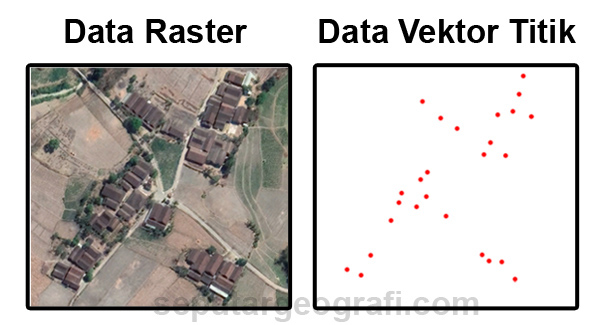
\includegraphics [height= 5cm]{image/data vektor titik}}
\caption{Perbedaan data raster dan data vektor
\citep{seputargeografi}}
\label{vektorkon}
\end{figure}

\section{pengindraan Jauh}

\textit{Remote sensing} adalah teknologi yang digunakan untuk mendapatkan informasi mengenai objek atau fenomena di permukaan bumi dari jarak jauh, tanpa perlu melakukan kontak langsung dengan objek tersebut \citep{putri2018analisis}. Teknologi ini dapat dimanfaatkan untuk berbagai keperluan, seperti pemetaan regional, pemantauan lingkungan, dan penelitian ilmiah. Data \textit{remote sensing} dapat dianggap sebagai sumber data yang sangat vital bagi Sistem Informasi Geografis (SIG) karena ketersediaannya secara teratur \citep{ghozali2016pemanfaatan}. Dengan beragam data \textit{remote sensing}, SIG memiliki kemampuan untuk menyediakan informasi yang akurat dan terkini mengenai kondisi permukaan Bumi. Teknologi pengindraan jauh berbasis satelit lebih sering digunakan untuk mengidentifikasi 
sesuatu. Kelebihan dari pengindraan jauh yaitu harganya bisa relatif lebih murah dan 
mudah didapatkan, adanya resolusi temporal (perulangan) hingga bisa digunakan 
untuk pemonitoran, dengan skala yang luas dan bisa menjangkau daerah yang kecil 
atau terpencil, bentuk datanya berupa digital hingga dapat digunakan untuk segala 
keperluan dan akan ditampilkan seperti yang diinginkan \citep{suwargana2010analisis}.

Dengan kemudahan yang ditawarkan oleh teknologi penginderaan jauh dan kehadiran \textit{drone}, proses memperoleh data spasial menjadi semakin mudah. Dalam penelitian ini, data citra udara yang diharapkan memiliki resolusi spasial yang tinggi sehingga dapat memperlihatkan detail objek dengan lebih rinci. Selain itu, diharapkan terdapat \textit{overlap} yang besar antara pasangan foto udara dan akurasi geometrik yang akurat. Citra udara dengan resolusi spasial tinggi dan overlap yang besar memungkinkan rekonstruksi model 3D permukaan bumi dengan ketelitian yang lebih baik. Akurasi geometrik yang akurat juga diperlukan untuk memastikan posisi objek di permukaan bumi dapat ditentukan dengan tepat dalam pengolahan data spasial selanjutnya.



\section{UAV (\textit{Unmanned Aerial Vehicle})}

\par \textit{Unmanned Aerial Vehicles} (UAV), yang lebih umum dikenal sebagai "\textit{Drone}", 
juga disebut sebagai robot terbang yang melibatkan pesawat udara tanpa awak (UAV) 
yang dapat terbang dalam jarak ribuan kilometer maupun \textit{drone} kecil yang terbang di
area terbatas. \textit{Drone} merupakan platform pemantauan jarak jauh yang baru, ekonomis, 
dan mudah digunakan, memberikan pengguna berbagai opsi terkait lokasi, waktu, dan 
metode pengumpulan citra serta data geospasial. pada penelitian ini drone yang digunakan adalah DJI Phantom 4 Pro yang dapat dilihat pada Gambar \ref{gambardrone}

% Menambahkan gambar 
\begin{figure}[H]
\centering
\frame{\includegraphics [height= 5cm]{image/DJI}}
\caption{\textit{Drone} DJI Phantom 4 Pro}
\label{gambardrone}
\end{figure}

\par \textit{Drone} telah menjadi alat yang sangat berharga dalam pemantauan jarak jauh dan pemetaan, menawarkan karakteristik unik dalam hal spasial, temporal, dan spektral. Salah satu keunggulan utama dalam hal spasial \textit{drone} adalah kemampuannya menghasilkan data dengan resolusi spasial yang sangat tinggi, memungkinkan pengumpulan informasi dengan tingkat detail yang luar biasa. Sebagai contoh, drone seperti DJI Phantom 4 Pro mampu mencapai resolusi spasial hingga 2,40 cm/pixel pada ketinggian terbang 90 meter \citep{hernina2019analisis}, suatu kemampuan yang sangat bermanfaat dalam pemetaan bidang tanah dan survei lapangan. Resolusi spasial yang optimal ini menjadikan \textit{drone} sebagai pelengkap ideal untuk metode survei konvensional, memungkinkan pembuatan peta lahan yang sangat akurat dan terperinci. Hubungan antara ketinggian terbang dan resolusi spasial yang dihasilkan dapat dilihat melalui tabel \ref{resolusispasial} yang menunjukkan resolusi spasial pada berbagai ketinggian menggunakan DJI Phantom 4 Pro, memberikan panduan berharga bagi para praktisi dalam merencanakan pemetaan mereka.

\begin{table}[H]
\centering
\caption{Resolusi spasial berdasarkan ketinggian terbang yang dapat dihasilkan pada Drone DJI Phantom 4 Pro \citep{hernina2019analisis}}
\label{resolusispasial}
\begin{tabular}{|l|l|l|}
\hline
\textbf{No.} & \textbf{Tinggi Terbang} & \textbf{Resolusi Spasial (cm/pixel)} \\ \hline
1.           & 90                      & 2,40                                 \\ \hline
2.           & 110                     & 2,97                                 \\ \hline
3.           & 130                     & 3,52                                 \\ \hline
4.           & 150                     & 4,09                                 \\ \hline
\end{tabular}
\end{table}

\par Drone tidak hanya unggul dalam aspek spasial, tetapi juga menawarkan keunggulan dalam karakteristik temporal dan spektral. Dari segi temporal, \textit{drone} memiliki kemampuan luar biasa dalam pengumpulan data secara \textit{real-time} dan efisien. Dengan kemampuan terbang dan mengakuisisi data dalam waktu yang relatif singkat, \textit{drone} menjadi solusi ideal untuk aplikasi survei lapangan yang membutuhkan data cepat dan akurat. Sementara itu, karakteristik spektral \textit{drone} memungkinkan pengumpulan data dalam berbagai spektrum elektromagnetik. Sebagai contoh, \textit{drone} seperti DJI Phantom 4 Pro dilengkapi dengan sensor kamera digital beresolusi tinggi 12 Megapixel, yang mampu menghasilkan data dengan tingkat detail yang mengesankan. Keunggulan ini terbukti dalam aplikasi pemetaan bidang tanah, di mana \textit{drone} menghasilkan orthofoto dengan ketelitian geometri yang sangat tinggi, menunjukkan perbedaan yang tidak signifikan dibandingkan dengan metode konvensional. Kombinasi karakteristik temporal dan spektral ini menjadikan \textit{drone} sebagai alat yang sangat efektif dan efisien dalam berbagai aplikasi pemetaan dan survei modern.

\textit{Drone} profesional untuk pemetaan juga dilengkapi dengan beragam jenis kamera canggih yang dirancang khusus untuk menghasilkan data berkualitas tinggi dan presisi. Kamera RGB standar dengan resolusi tinggi, biasanya mulai dari 12MP hingga 100MP atau lebih, merupakan pilihan umum untuk menghasilkan gambar berwarna natural dengan detail yang tajam. Untuk aplikasi yang lebih spesifik, kamera multispektral dan hiperspektral menjadi pilihan utama. Kamera multispektral, yang menangkap data dalam beberapa band spektral termasuk inframerah dekat (NIR), sangat bermanfaat untuk analisis vegetasi dan pertanian presisi. Sementara itu, kamera hiperspektral, dengan kemampuannya mengumpulkan data dalam ratusan band spektral yang sangat sempit, ideal untuk analisis mineral dan aplikasi lingkungan yang kompleks.

Selain itu, \textit{drone} profesional juga sering dilengkapi dengan kamera termal untuk menangkap data suhu permukaan, yang berguna dalam inspeksi bangunan dan pemantauan kebakaran hutan. Teknologi LiDAR (\textit{Light Detection and Ranging}) juga semakin populer dalam pemetaan \textit{drone}, menggunakan laser untuk menghasilkan model elevasi digital yang sangat akurat, ideal untuk pemetaan topografi dan pemodelan 3D perkotaan. Untuk aplikasi khusus seperti pemodelan 3D perkotaan dan inspeksi infrastruktur, kamera oblique yang dapat mengambil gambar dari berbagai sudut menjadi pilihan yang tepat. Terakhir, kamera 360° juga mulai digunakan dalam \textit{drone} pemetaan untuk menghasilkan gambar panorama yang berguna dalam pembuatan virtual tour dan dokumentasi lokasi secara komprehensif. Pemilihan jenis kamera pada \textit{drone} profesional untuk pemetaan sangat bergantung pada tujuan spesifik proyek, kondisi lingkungan, dan kebutuhan data yang ingin diperoleh, dengan banyak platform \textit{drone} modern memungkinkan penggantian payload untuk fleksibilitas maksimal.


\section{Perencanaan jalur terbang \textit{Drone}}

Perencanaan jalur terbang \textit{drone} merupakan aspek krusial dalam pemetaan fotogrametri. Perencanaan yang tepat sangat penting untuk menghasilkan data pemetaan yang akurat dan efisien, dengan mempertimbangkan faktor-faktor seperti luas area, resolusi yang diinginkan, dan prosedur yang ditentukan, karena jika ada salah satu tahap pembuatan jalur terbang yang terlewat maka akan mempengaruhi hasil akhir \citep{guntara2015perencanaan}. Salah satu metode yang digunakan dalam perancangan jalur terbang adalah metode waypoint. Metode ini melibatkan penentuan titik-titik koordinat yang akan dilalui oleh \textit{drone} selama penerbangan, memungkinkan kontrol yang lebih presisi atas rute penerbangan dan area cakupan. Dalam berbagai aplikasi, pemanfaatan data \textit{drone} telah dikaji untuk berbagai bidang. Desain jalur terbang yang tepat sangat penting untuk menghasilkan data yang akurat dalam pemetaan area, inventarisasi objek, dan pemantauan kondisi lingkungan. Untuk berbagai jenis wilayah, optimalisasi perencanaan jalur terbang UAV perlu mempertimbangkan kondisi topografi, batasan regulasi, dan faktor lingkungan seperti angin. Untuk area dengan topografi yang bervariasi, penggunaan mode penerbangan \textit{terrain following} disarankan, di mana \textit{drone} menjaga ketinggian relatif yang konstan terhadap permukaan tanah. Pendekatan ini memungkinkan adaptasi terhadap berbagai kondisi lapangan dan memastikan kualitas data yang konsisten.

Faktor-faktor yang mempengaruhi kualitas hasil pemetaan juga perlu diperhatikan dalam desain jalur terbang. Analisis menunjukkan beberapa temuan penting. Pertama, ketinggian terbang berbanding terbalik dengan ketelitian peta, di mana semakin rendah ketinggian terbang, semakin tinggi ketelitian yang dihasilkan. Kedua, kecepatan \textit{Drone} yang lebih rendah cenderung menghasilkan peta yang lebih teliti, meskipun hal ini perlu diimbangi dengan pertimbangan efisiensi waktu penerbangan. Terakhir, \textit{overlap} foto memiliki pengaruh signifikan, dengan \textit{overlap} yang lebih besar (80\% frontal \textit{overlap} dan 60\% - 70\% \textit{side overlap}) menghasilkan ketelitian yang lebih baik dibandingkan dengan overlap yang lebih kecil dan lebih membantu dalam proses stitching foto dan meningkatkan akurasi rekonstruksi 3D \citep{torres2018assessing}. Dalam aspek regulasi, penting untuk memperhatikan peraturan penerbangan drone yang berlaku di Indonesia, termasuk batas ketinggian maksimum dan area terbang yang diizinkan, Dengan mempertimbangkan semua faktor ini, desain jalur terbang yang optimal dapat menghasilkan data pemetaan yang akurat dan efisien, sesuai dengan kebutuhan spesifik proyek dan kondisi lapangan di Indonesia.

\section{Mosaik}

\par Mosaik citra spasial yang diambil menggunakan \textit{drone} melibatkan serangkaian proses kompleks yang terjadi di latar belakang aplikasi. Proses ini dimulai dengan akuisisi citra, di mana drone mengambil serangkaian foto yang tumpang tindih, biasanya dengan overlap 60-80\% untuk memastikan area yang cukup untuk pencocokan fitur. Setelah citra diperoleh, langkah berikutnya adalah ekstraksi dan pencocokan fitur. Dalam tahap ini, algoritma \textit{computer vision} seperti SIFT atau SURF digunakan untuk mengidentifikasi dan mencocokkan fitur-fitur unik antar citra yang tumpang tindih seperti yang terlihat pada Gambar \ref{mosaik}, memungkinkan aplikasi untuk menentukan hubungan spasial antar citra \citep{ghosh2016survey}.

\begin{figure}[H]
\centering
\frame{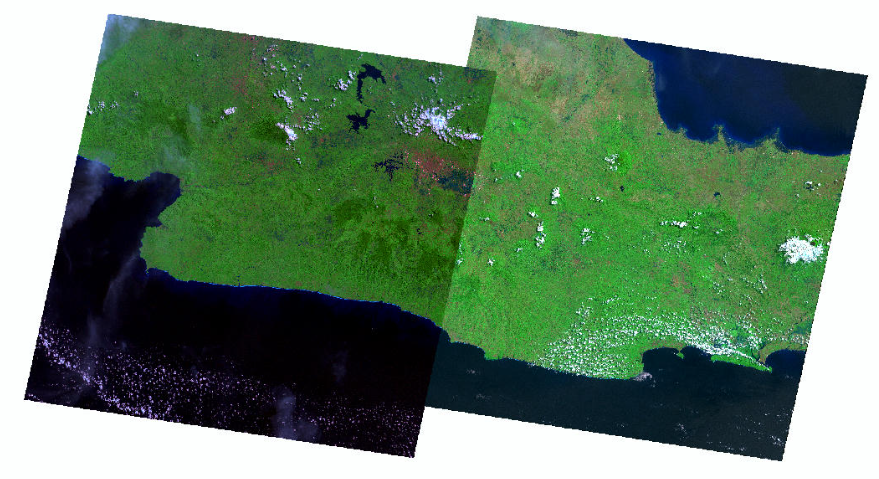
\includegraphics [height= 5cm]{image/mosaik}}
\caption{Ilustrasi proses mosaik pada citra udara}
\label{mosaik}
\end{figure}

Dalam proses ekstraksi dan pencocokan fitur, dua algoritma \textit{computer vision} yang sering digunakan adalah SIFT (\textit{Scale-Invariant Feature Transform}) dan SURF (\textit{Speeded Up Robust Features}). SIFT yang diperkenalkan oleh Lowe pada tahun 1999, adalah algoritma yang mampu mendeteksi dan mendeskripsikan fitur lokal dalam gambar. Keunggulan utama SIFT terletak pada kemampuannya untuk mengenali fitur yang \textit{invariant} terhadap skala, rotasi, dan sebagian besar terhadap perubahan pencahayaan dan sudut pandang 3D. Ini membuat SIFT sangat cocok untuk pencocokan fitur dalam citra drone yang diambil dari berbagai sudut dan ketinggian \citep{lowe2004distinctive}. Di sisi lain, SURF, yang dikembangkan oleh Bay et al. pada tahun 2006, dirancang sebagai versi yang lebih cepat dan lebih efisien dari SIFT. Meskipun sedikit kurang akurat dibandingkan SIFT dalam beberapa kasus, SURF umumnya lebih cepat dan masih cukup tangguh untuk banyak aplikasi pembuatan mosaik citra drone \citep{bay2006surf}.

Meskipun proses ini umumnya otomatis, tantangan seperti variasi pencahayaan, pergerakan objek, dan kompleksitas \textit{terrain} dapat mempengaruhi kualitas hasil akhir. Namun, pengembangan terbaru dalam \textit{machine learning} dan \textit{computer vision} terus meningkatkan akurasi dan efisiensi proses mosaik, menjanjikan hasil yang lebih baik di masa depan.


\section{\textit{Ground Control Point} (GCP)}

 GCP (\textit{Ground Control Point}) atau titik kontrol tanah adalah penandaan tempat yang terkoordinasi dalam bentuk beberapa titik yang diperlukan untuk mengoreksi data dan meningkatkan citra umum, yang disebut proses koreksi GCP, terdiri dari sepasang X dan koordinat Y yang terdiri dari koordinat asal dan referensi koordinat. Keakuratan GCP sangat bergantung pada jenis GPS yang digunakan dan jumlah sampel GCP di lokasi dan waktu pengambilan \citep{widodo2023pemanfaatan}. Dalam pemetaan menggunakan \textit{drone}, \textit{Ground Control Points} (GCP) menjadi elemen kunci untuk memastikan akurasi dan konsistensi hasil. Meskipun \textit{drone} dilengkapi dengan sensor GPS, seringkali tidak dapat memberikan akurasi yang memadai untuk aplikasi pemetaan yang presisi. Melalui pemasangan GCP di area yang akan dipetakan, kita dapat memperbaiki distorsi geometrik pada citra \textit{drone} dan menjamin bahwa citra tersebut terdaftar dengan benar ke koordinat geografis yang tepat. Hal ini tidak hanya meningkatkan akurasi pemetaan secara keseluruhan, tetapi juga memungkinkan perbandingan dan analisis yang konsisten antara citra dari berbagai penerbangan atau sumber data. Dengan demikian, penggunaan GCP menjadi suatu keharusan dalam pemetaan menggunakan \textit{drone} untuk aplikasi yang memerlukan presisi dan konsistensi spasial yang tinggi. berikut contoh \textit{Ground Control Point} (GCP) yang digunakan dalam proses pemetaan yang ditampilkan pada Gambar 2.3.

 \begin{figure}[H]
\centering
\frame{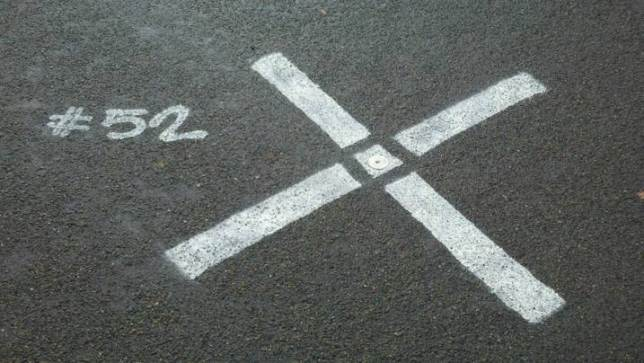
\includegraphics [height= 5cm]{image/x-gcp-contour-lines}}
\caption{\textit{Ground Control Point} di lapangan survei}
\label{dig_facenet}
\end{figure}

\section{Matriks Evaluasi}

\par Matriks evaluasi pada mosaik citra memberikan informasi kuantitatif tentang akurasi geometrik. Kombinasi beberapa matriks evaluasi ini memungkinkan perbandingan yang komprehensif antara hasil mosaik dari berbagai perangkat lunak atau metode pemrosesan yang berbeda.

\subsection{\textit{Root Mean Square Error} (RMSE)}
    \textit{Root Mean Square Error} (RMSE) merupakan metrik evaluasi yang umum digunakan untuk mengukur akurasi hasil mosaik citra spasial, terutama yang diperoleh dari pencitraan drone. Dalam konteks pemetaan drone, kita sering menggunakan dua jenis RMSE, yaitu RMSEr untuk akurasi horizontal dan RMSEz untuk akurasi vertikal. RMSEr (\textit{Root Mean Square Error radial}) mengukur akurasi posisional horizontal dengan menggabungkan error dalam arah x (longitude) dan y (latitude), sedangkan RMSEz (\textit{Root Mean Square Error in} z) mengukur akurasi vertikal atau elevasi. RMSE menghitung rata-rata perbedaan kuadrat antara nilai yang diprediksi (dalam hal ini, koordinat piksel pada citra mosaik) dan nilai yang sebenarnya (koordinat referensi di lapangan), kemudian mengambil akar kuadratnya. Dalam konteks mosaik citra \textit{drone}, RMSE digunakan untuk menilai sejauh mana citra hasil mosaik menyimpang dari posisi sebenarnya di permukaan bumi. Semakin rendah nilai RMSE, semakin tinggi akurasi geometris dari mosaik yang dihasilkan. RMSE dan RMSEr dihitung dengan rumus seperti pada Gambar \ref{rumus_rmse}, \ref{rumus_rmser} berikut:

    \begin{figure}[H]
    \centering
    \frame{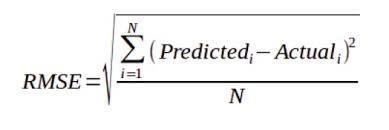
\includegraphics [height= 2cm]{image/RMSE1.jpg}}
    \caption{Rumus Root Mean Square Error \citep{geeksforgeeksRMSE}}
    \label{rumus_rmse}
    \end{figure}

    \begin{figure}[H]
    \centering
    \frame{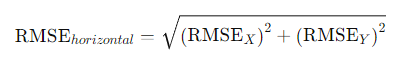
\includegraphics [height= 2cm]{rumusrmser.png}}
    \caption{Rumus Root Mean Square Error Radial (RMSEr)}
    \label{rumus_rmser}
    \end{figure}
    
    Seperti yang terlihat pada Gambar \ref{rumus_rmse} yang mana '\textit{predicted}' adalah koordinat pada citra mosaik, '\textit{actual}' adalah koordinat referensi di lapangan, dan 'n' adalah jumlah titik sampel \citep{jaud2016assessing}. Penggunaan RMSE dalam evaluasi mosaik citra drone telah banyak diterapkan dalam berbagai studi. Misalnya, dalam pemetaan topografi menggunakan citra drone, RMSE horizontal berkisar antara 5,5 cm hingga 6,9 cm, tergantung pada ketinggian terbang drone \citep{aguera2017assessment}. RMSE juga digunakan untuk membandingkan akurasi mosaik citra yang dihasilkan dari berbagai perangkat lunak fotogrametri. Penelitian menunjukkan bahwa pemilihan perangkat lunak dan metode pengolahan dapat mempengaruhi nilai RMSE akhir dari mosaik yang dihasilkan \citep{padro2019comparison}. 
    

%     \begin{table}[h]
% \centering
% \caption{Skala Peta Dasar dan Nilai GSD}
% \begin{tabular}{|c|c|}
% \hline
% Skala Peta Dasar & Nilai GSD (cm) \\
% \hline
% 1:10.000 & $\leq$ 30 \\
% \hline
% 1:5.000 & $\leq$ 15 \\
% \hline
% 1:2.500 & $\leq$ 10 \\
% \hline
% 1:1.000 & $\leq$ 8 \\
% \hline
% \end{tabular}
% \label{tab:skala-gsd}
% \end{table}

\subsection{\textit{Circular Error} 90\% (CE90) dan \textit{Linear Error} 90\% (LE90)}

    \textit{Circular Error} (CE90) dan \textit{Linear Error} (LE90) merupakan parameter penting dalam mengevaluasi akurasi geometrik dari citra hasil pemetaan udara, termasuk mosaik citra yang dihasilkan dari pengambilan gambar menggunakan \textit{drone}. Kedua parameter ini sering digunakan untuk mengukur tingkat presisi posisional dari data geospasial. \textit{Circular Error} 90 (CE90) didefinisikan sebagai radius lingkaran yang mencakup 90\% dari titik-titik data yang diukur relatif terhadap posisi sebenarnya. Dalam konteks mosaik citra drone, CE90 menggambarkan akurasi horizontal dari citra yang dihasilkan. Semakin kecil nilai CE90, semakin tinggi akurasi posisional horizontal citra tersebut \citep{peppa2019photogrammetric}. \textit{Linear Error} 90 (LE90), di sisi lain, mengukur akurasi vertikal. LE90 didefinisikan sebagai interval vertikal yang mencakup 90\% dari perbedaan elevasi antara titik-titik yang diukur dengan nilai elevasi sebenarnya. Dalam konteks mosaik citra drone, LE90 sangat penting untuk menilai akurasi model elevasi digital yang dihasilkan dari data penginderaan jauh \citep{wolf2002elementary}. CE90 dan LE90 dihitung menggunakan rumus seperti pada Gambar \ref{rumus_ce}.

    \begin{figure}[H]
    \centering
    \frame{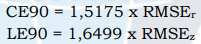
\includegraphics [height= 2cm]{rumus cele.png}}
    \caption{Rumus CE90 dan LE90 \citep{BIG2014}}
    \label{rumus_ce}
    \end{figure}

    Penggunaan CE90 dan LE90 dalam evaluasi mosaik citra drone memungkinkan penilaian yang lebih komprehensif terhadap kualitas geometrik hasil pemetaan. Studi menunjukkan bahwa penggunaan \textit{drone} dengan sensor kamera beresolusi tinggi dapat menghasilkan mosaik ortofoto dengan CE90 kurang dari 10 cm dan LE90 kurang dari 15 cm, mendemonstrasikan potensi tinggi dari teknologi \textit{drone} untuk pemetaan presisi tinggi \citep{kalantar2017drone}. Namun, perlu dicatat bahwa akurasi yang dicapai dapat bervariasi tergantung pada berbagai faktor seperti kualitas kamera, ketinggian terbang, kondisi cuaca, dan metode pengolahan data. Oleh karena itu, analisis CE90 dan LE90 penting dilakukan dalam setiap proyek pemetaan drone \citep{sanz2018accuracy}. Penting untuk dicatat bahwa interpretasi CE90 dan LE90 harus mempertimbangkan resolusi spasial citra asli dan skala peta yang diinginkan.

    Di Indonesia, standar ketelitian peta diatur oleh Badan Informasi Geospasial (BIG) melalui Peraturan Kepala BIG Nomor 6 Tahun 2018 tentang Pedoman Teknis Ketelitian Peta Dasar seperti pada Tabel \ref{tab:ketelitian-peta-rbi}. Standar ini penting diperhatikan dalam pembuatan mosaik citra dari drone untuk memastikan hasil pemetaan memenuhi kriteria ketelitian nasional.

    \begin{table}[h]
\centering
\caption{Ketelitian Peta RBI}
\label{tab:ketelitian-peta-rbi}
\resizebox{\textwidth}{!}{
\begin{tabular}{|c|c|c|c|c|c|c|c|c|}
\hline
\multirow{3}{*}{No} & \multirow{3}{*}{Skala} & \multirow{3}{*}{\begin{tabular}[c]{@{}c@{}}Interval\\ Kontur\\ (m)\end{tabular}} & \multicolumn{6}{c|}{Ketelitian Peta RBI} \\
\cline{4-9}
 &  &  & \multicolumn{2}{c|}{Kelas 1} & \multicolumn{2}{c|}{Kelas 2} & \multicolumn{2}{c|}{Kelas 3} \\
\cline{4-9}
 &  &  & \begin{tabular}[c]{@{}c@{}}Horisontal\\ (CE90\\ dalam m)\end{tabular} & \begin{tabular}[c]{@{}c@{}}Vertikal\\ (LE90\\ dalam\\ m)\end{tabular} & \begin{tabular}[c]{@{}c@{}}Horisontal\\ (CE90\\ dalam m)\end{tabular} & \begin{tabular}[c]{@{}c@{}}Vertikal\\ (LE90\\ dalam m)\end{tabular} & \begin{tabular}[c]{@{}c@{}}Horisontal\\ (CE90\\ dalam m)\end{tabular} & \begin{tabular}[c]{@{}c@{}}Vertikal\\ (LE90\\ dalam\\ m)\end{tabular} \\
\hline
1 & 1:1.000.000 & 400 & 300 & 200 & 600 & 300 & 900,0 & 400 \\
\hline
2 & 1:500.000 & 200 & 150 & 100 & 300 & 150 & 450,0 & 200 \\
\hline
3 & 1:250.000 & 100 & 75 & 50 & 150 & 75 & 225,0 & 100 \\
\hline
4 & 1:100.000 & 40 & 30 & 20 & 60 & 30 & 90,0 & 40 \\
\hline
5 & 1:50.000 & 20 & 15 & 10 & 30 & 15 & 45,0 & 20 \\
\hline
6 & 1:25.000 & 10 & 7,5 & 5 & 15 & 7,5 & 22,5 & 10 \\
\hline
7 & 1:10.000 & 4 & 3 & 2 & 6 & 3 & 9,0 & 4 \\
\hline
8 & 1:5.000 & 2 & 1,5 & 1 & 3 & 1,5 & 4,5 & 2 \\
\hline
9 & 1:2.500 & 1 & 0,75 & 0,5 & 1,5 & 0,75 & 2,3 & 1 \\
\hline
10 & 1:1.000 & 0,4 & 0,3 & 0,2 & 0,6 & 0,3 & 0,9 & 0,4 \\
\hline
\end{tabular}
}
\end{table}

    






\section{Penelitian Terkait}

\par Penelitian yang dilakukan oleh Petrus Krisologus Hamur dkk.(2019) yang membahas tentang "Kajian pengolahan data foto udara menggunakan perangkat lunak Agisoft Photoscan dan PIX4D Mapper". Dalam penelitian ini, pemrosesan data foto udara dilakukan menggunakan perangkat lunak Agisoft Photoscan dan Pix4D Mapper, melibatkan sebanyak 158 foto dan 8 titik \textit{Ground Control Point} (GCP). Untuk menguji akurasi posisi horizontal dan vertikal, akan diterapkan metode perhitungan yang diacu dari Peraturan Badan Informasi Geospasial (BIG) No. 15 tahun 2014. Sementara itu, uji ketelitian objek pada Orthofoto akan melibatkan interpretasi dan perhitungan dengan menerapkan metode persamaan omisi komisi. Dari hasil penelitian akurasi data \textit{Digital Elevation Model} (DEM) dan Orthofoto, dengan merujuk pada standar yang ditetapkan dalam Peraturan BIG No. 15 tahun 2014, ditemukan bahwa nilai \textit{Linear Error} 90\% (LE90) dari Agisoft Photoscan adalah sekitar 0.279 m, sedangkan Pix4D Mapper mencapai 0.509 m. Demikian pula, nilai \textit{Circular Error} 90\% (CE90) dari Agisoft Photoscan adalah sekitar 0.139 m, sementara Pix4D Mapper sebesar 0.224 m. Lebih lanjut, dalam menguji akurasi objek dari data Orthofoto menggunakan metode omisi komisi, hasil perhitungan menunjukkan bahwa presentase rata-rata akurasi objek dari kedua perangkat lunak, Agisoft Photoscan dan Pix4D Mapper, melebihi 90\%. Keakuratan ini memenuhi standar yang disyaratkan, yaitu lebih dari 85\%. Penelitian ini secara keseluruhan memberikan pemahaman yang mendalam mengenai kemampuan Agisoft Photoscan dan Pix4D Mapper dalam menghasilkan data DEM dan Orthofoto yang memenuhi kriteria akurasi geometri dan objek yang telah ditetapkan \citep{hamur2019kajian}.

Penelitian yang dilakukan oleh Sultan Alifian Hapriansyah dkk. (2021) yang membahas tentang "Analisis perbandingan ketelitian hasil orthomosaic menggunakan perangkat lunak komersial PIX4Dmapper dan open source WebODM" yang menyajikan penelitian dan hasil sebagai berikut. Foto tegak merupakan hasil pengambilan gambar dari pesawat atau UAV yang memiliki sumbu optik kamera yang berorientasi vertikal atau hampir vertikal. Orthomosaic, yang diperoleh dari pengolahan foto udara menggunakan perangkat lunak fotogrametri khusus, menjadi fokus dalam penelitian ini. Penelitian ini menggunakan data foto udara dan GPS wilayah Kebonwaris, Kecamatan Pandaan, Pasuruan - Jawa Timur. WenODM dan versi uji coba Pix4Dmapper digunakan sebagai perangkat lunak pembanding. Proses pengolahan data dimulai dari langkah-langkah impor gambar, impor titik kontrol, pembentukan awan titik, pembentukan mesh, pembentukan model permukaan, hingga pembentukan orthomosaic. Pix4Dmapper memberikan nilai \textit{Root Mean Square Error} (RMSe) horizontal sekitar 0,67361672 dan RMSe vertikal sekitar 0,664288006. Sementara itu, WebODM memberikan nilai ketelitian dengan RMSe horizontal sekitar 1,92810327 dan RMSe vertikal sekitar 1,195321336. Resolusi yang diperoleh dari WebODM adalah sekitar 5,5cm/piksel, sedangkan Pix4Dmapper sekitar 6,4cm/piksel. Dari hasil analisis, dapat disimpulkan bahwa Pix4Dmapper unggul dalam hal ketelitian yang diperoleh, sementara WebODM memiliki keunggulan dalam resolusi \citep{hapriansyah2021analisis}.

Penelitian yang dilakukan oleh Hadiwijaya Lesmana Salim dkk. (2018) yang membahas tentang "Pemetaan dinamika hutan mangrove menggunakan \textit{drone} dan pengindraan jauh di P. Rambut, Kepulauan Seribu" yang menyajikan penelitian dan pengamatan terhadap sebaran dan luas hutan mangrove di Pulau Rambut Pada bulan November 2017 dan Juli 2010. Pengamatan ini melibatkan analisis foto udara dan citra Geo Eye 1. Untuk memvalidasi data lapangan, dilakukan kunjungan lapangan. Metode yang diterapkan dalam penelitian ini adalah segementasi dan klasifikasi terbimbing menggunakan pendekatan analisis berbasis objek (OBIA). Berdasarkan hasil analisis foto udara, data citra, dan validasi lapangan, dapat diestimasi bahwa pada tahun 2010, luas hutan mangrove di Pulau Rambut mencapai 16,73 ha, sementara pada tahun 2017 mencapai 17,48 ha, menunjukkan peningkatan sebesar 0,75 ha. Hutan mangrove di Pulau Rambut terdiri dari 10 jenis, dengan dominasi jenis \textit{Rhizophora mucronata}. Penelitian ini menyimpulkan bahwa analisis berbasis objek terhadap foto udara yang diambil dengan \textit{drone} menghasilkan pemetaan dinamika hutan mangrove yang lebih baik dibandingkan dengan penggunaan citra satelit Geo Eye 1. Akurasi keseluruhan mencapai 77,3\%, dan nilai koefisien kappa sebesar 0,62 \citep{islands2018pemetaan}.
% \fancyhf{} 
% \fancyfoot[R]{\thepage}

\begin{comment}
\bibliography{daftar-pustaka}
\end{comment}


\fancyhf{} 
\fancyfoot[R]{\thepage}

%-------------------------------------------------------------------------------
%                            BAB III
%               		METODOLOGI PENELITIAN
%-------------------------------------------------------------------------------
% \fancyhf{} 
% \fancyfoot[R]{\thepage}
\chapter{METODE PENENILITIAN}
%\thispagestyle{plain} % Halaman pertama bab menggunakan gaya plain
\section{Deskripsi Lokasi Penelitian}
Lokasi kampus II USK terdiri dari 4 kecamatan (Baitussalam, Mesjid Raya, 
Darussalam, Kuta Baro), namun penelitian ini hanya memfokuskan pada Kecamatan 
Mesjid raya yang merupakan bagian tanah Kampus II USK sesuai dengan prioritas
kebutuhan tanah untuk lokasi pengembangan kampus seluas 250 Ha, Gambar \ref{batas dan area studi} menunjukan batas tanah Kampus II USK dan area studi penelitian.

\begin{figure}[H]
\centering
\frame{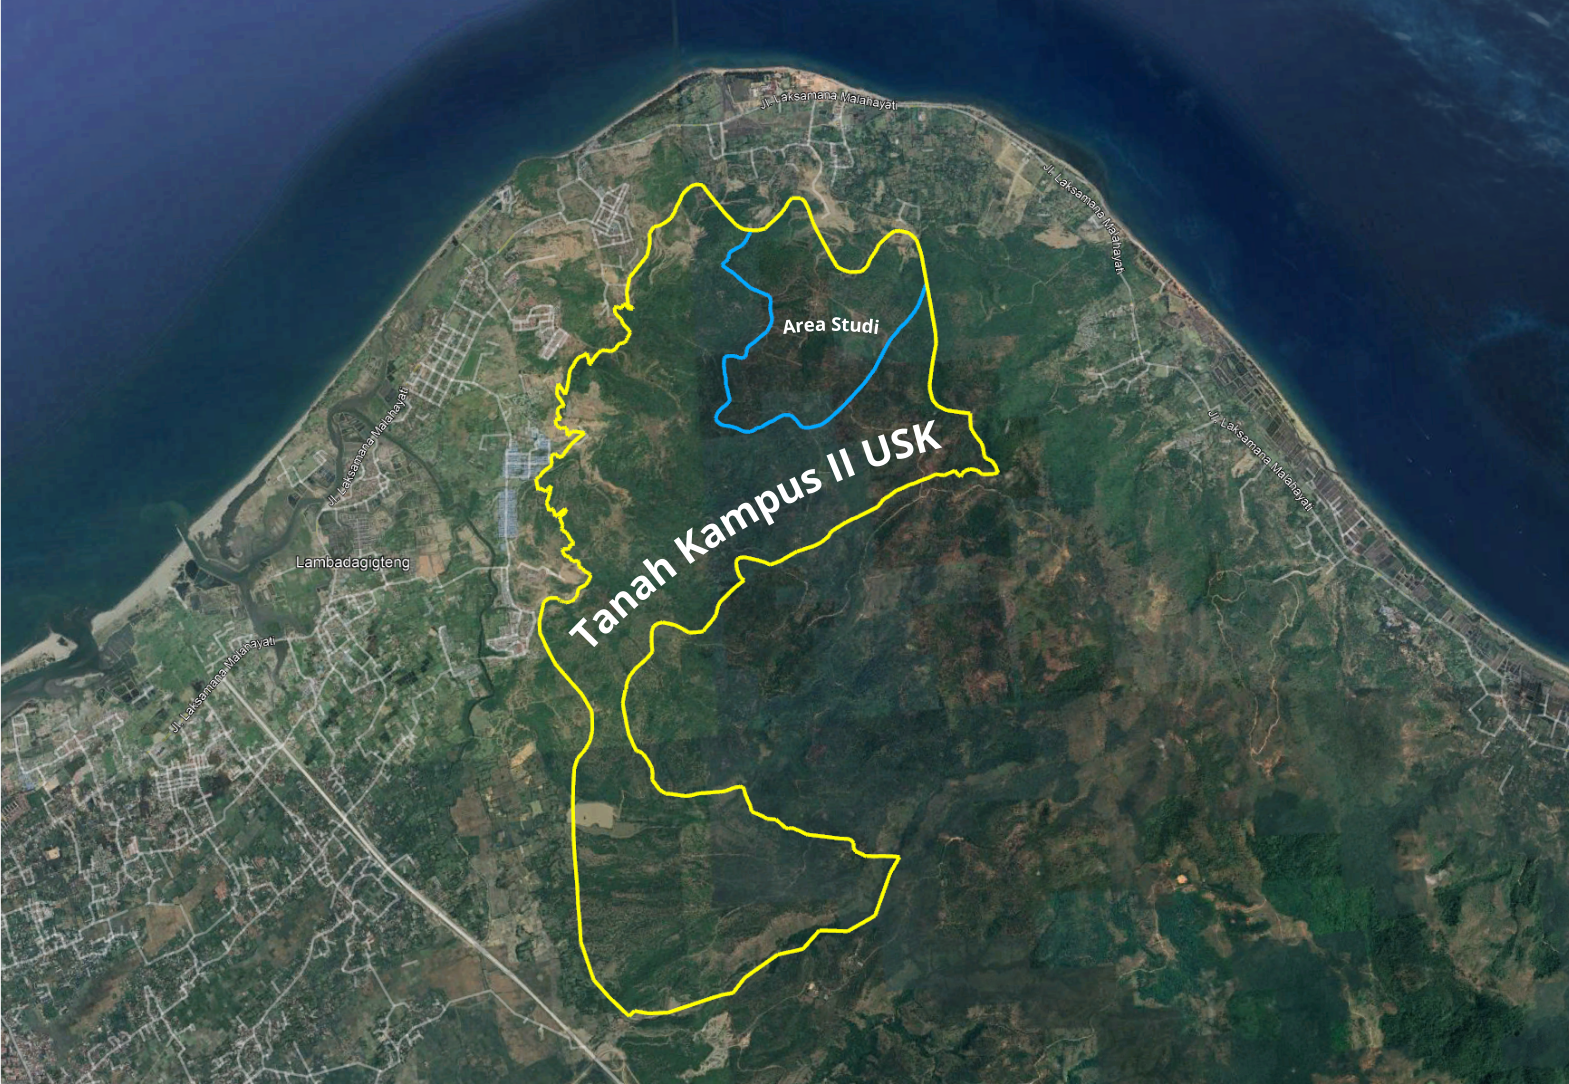
\includegraphics [width = 9cm]{image/Tanah Kampus II USK}}
\caption{Batas tanah kampus II USK seluas 1.588 Ha (kuning), dan batas area studi penelitian seluas 250 Ha (biru)
}
\label{batas dan area studi}
\end{figure}

\section{Waktu dan Lokasi Penelitian}
Penelitian ini dilaksanakan mulai dari bulan Maret hingga Agustus 2024, melibatkan serangkaian aktivitas di laboratorium. Kegiatan laboratorium melibatkan proses pengolahan citra, yang dilakukan di Laboratorium Terpadu Sistem Informasi Geografis dan Data Spasial USK. Rincian jadwal penelitian dapat dilihat pada Tabel 3.1 berikut.

% Please add the following required packages to your document preamble:
% \usepackage{multirow}
% \usepackage[table,xcdraw]{xcolor}
% Beamer presentation requires \usepackage{colortbl} instead of \usepackage[table,xcdraw]{xcolor}
\begin{table}[H]
  \caption{Distribusi Jadwal Kegiatan Penelitian Bulan Maret-Agustus 2024}
  \label{tab:jadwal-kegiatan-januari-maret-2024}
  \resizebox{\columnwidth}{!}{%
  \begin{tabular}{|c|l|llll|llll|llll|llll|llll|llll|}
  \hline
                       & \multicolumn{1}{c|}{}                           & \multicolumn{4}{c|}{Maret}                                                                                                                                             & \multicolumn{4}{c|}{April}                                                                                                                                            & \multicolumn{4}{c|}{Mei}                                                                                                                                               & \multicolumn{4}{c|}{Juni}                                                                                                                                                                                             & \multicolumn{4}{c|}{Juli}                                                                                                                                                 & \multicolumn{4}{c|}{Agustus}                                                                                                                                                \\ \cline{3-26} 
                       & \multicolumn{1}{c|}{}                           & \multicolumn{4}{c|}{Minggu Ke-}                                                                                                                                          & \multicolumn{4}{c|}{Minggu Ke-}                                                                                                                                          & \multicolumn{4}{c|}{Minggu Ke-}                                                                                                                                          & \multicolumn{4}{c|}{Minggu Ke-}                                                                                                                                                                                        & \multicolumn{4}{c|}{Minggu Ke-}                                                                                                                                          & \multicolumn{4}{c|}{Minggu Ke-}                                                                                                                                          \\ \cline{3-26} 
  \multirow{-3}{*}{No} & \multicolumn{1}{c|}{\multirow{-3}{*}{Kegiatan}} & \multicolumn{1}{c|}{1}                        & \multicolumn{1}{c|}{2}                        & \multicolumn{1}{c|}{3}                        & \multicolumn{1}{c|}{4}   & \multicolumn{1}{c|}{1}                        & \multicolumn{1}{c|}{2}                        & \multicolumn{1}{c|}{3}                        & \multicolumn{1}{c|}{4}   & \multicolumn{1}{c|}{1}                        & \multicolumn{1}{c|}{2}                        & \multicolumn{1}{c|}{3}                        & \multicolumn{1}{c|}{4}   & \multicolumn{1}{c|}{1}                                               & \multicolumn{1}{c|}{2}                                               & \multicolumn{1}{c|}{3}                        & \multicolumn{1}{c|}{4}   & \multicolumn{1}{c|}{1}                        & \multicolumn{1}{c|}{2}                        & \multicolumn{1}{c|}{3}                        & \multicolumn{1}{c|}{4}   & \multicolumn{1}{c|}{1}                        & \multicolumn{1}{c|}{2}                        & \multicolumn{1}{c|}{3}                        & \multicolumn{1}{c|}{4}   \\ \hline
  
  1                    & Studi Literatur                                 & \multicolumn{1}{l|}{\cellcolor[HTML]{656565}} & \multicolumn{1}{l|}{\cellcolor[HTML]{656565}} & \multicolumn{1}{l|}{\cellcolor[HTML]{656565}} & \cellcolor[HTML]{656565} & \multicolumn{1}{l|}{\cellcolor[HTML]{656565}} & \multicolumn{1}{l|}{\cellcolor[HTML]{656565}} & \multicolumn{1}{l|}{\cellcolor[HTML]{656565}} & \cellcolor[HTML]{656565} & \multicolumn{1}{l|}{\cellcolor[HTML]{656565}} & \multicolumn{1}{l|}{\cellcolor[HTML]{656565}} & \multicolumn{1}{l|}{\cellcolor[HTML]{656565}} & \cellcolor[HTML]{656565} & \multicolumn{1}{l|}{}                                                & \multicolumn{1}{l|}{}                                                & \multicolumn{1}{l|}{}                         &                          & \multicolumn{1}{l|}{}                         & \multicolumn{1}{l|}{}                         & \multicolumn{1}{l|}{}                         &                          & \multicolumn{1}{l|}{}                         & \multicolumn{1}{l|}{}                         & \multicolumn{1}{l|}{}                         &                          \\ \hline
  2                    & Analisis Akuisisi Data                                & \multicolumn{1}{l|}{}                         & \multicolumn{1}{l|}{}                         & \multicolumn{1}{l|}{}                         & & \multicolumn{1}{l|}{\cellcolor[HTML]{656565}} & \multicolumn{1}{l|}{\cellcolor[HTML]{656565}}                         & \multicolumn{1}{l|}{\cellcolor[HTML]{656565}}                         &                          \cellcolor[HTML]{656565}& \multicolumn{1}{l|}{\cellcolor[HTML]{656565}} & \multicolumn{1}{l|}{\cellcolor[HTML]{656565}}                         & \multicolumn{1}{l|}{\cellcolor[HTML]{656565}}                         &                          \cellcolor[HTML]{656565}& \multicolumn{1}{l|}{\cellcolor[HTML]{656565}}                                                & \multicolumn{1}{l|}{}                                                & \multicolumn{1}{l|}{}                         &                          & \multicolumn{1}{l|}{}                         & \multicolumn{1}{l|}{}                         & \multicolumn{1}{l|}{}                         &                          & \multicolumn{1}{l|}{}                         & \multicolumn{1}{l|}{}                         & \multicolumn{1}{l|}{}                         &                          \\ \hline
  3                    & Pengumpulan Data                              & \multicolumn{1}{l|}{}                         & \multicolumn{1}{l|}{}                         & \multicolumn{1}{l|}{}                         &                          & \multicolumn{1}{l|}{} & \multicolumn{1}{l|}{} & \multicolumn{1}{l|}{} &                          & \multicolumn{1}{l|}{}                         & \multicolumn{1}{l|}{}                         & \multicolumn{1}{l|}{}                         &                          \cellcolor[HTML]{656565}& \multicolumn{1}{l|}{\cellcolor[HTML]{656565}}                                                & \multicolumn{1}{l|}{\cellcolor[HTML]{656565}}                                                & \multicolumn{1}{l|}{}                         &                          & \multicolumn{1}{l|}{}                         & \multicolumn{1}{l|}{}                         & \multicolumn{1}{l|}{}                         &                          & \multicolumn{1}{l|}{}                         & \multicolumn{1}{l|}{}                         & \multicolumn{1}{l|}{}                         &                          \\ \hline
  4                    & Mosaik Menggunakan Agisoft Metashape                     & \multicolumn{1}{l|}{}                         & \multicolumn{1}{l|}{}                         & \multicolumn{1}{l|}{}                         &                          & \multicolumn{1}{l|}{}                         & \multicolumn{1}{l|}{}                         & \multicolumn{1}{l|}{} & & \multicolumn{1}{l|}{} & \multicolumn{1}{l|}{} & \multicolumn{1}{l|}{} & & \multicolumn{1}{l|}{\cellcolor[HTML]{656565}}                                                & \multicolumn{1}{l|}{\cellcolor[HTML]{656565}}                                                & \multicolumn{1}{l|}{\cellcolor[HTML]{656565}}                         &                          \cellcolor[HTML]{656565}& \multicolumn{1}{l|}{}                         & \multicolumn{1}{l|}{}                         & \multicolumn{1}{l|}{}                         &                          & \multicolumn{1}{l|}{}                         & \multicolumn{1}{l|}{}                         & \multicolumn{1}{l|}{}                         &                          \\ \hline
  5                    & Mosaik Menggunakan PIX4Dmapper                                  & \multicolumn{1}{l|}{}                         & \multicolumn{1}{l|}{}                         & \multicolumn{1}{l|}{}                         &                          & \multicolumn{1}{l|}{}                         & \multicolumn{1}{l|}{}                         & \multicolumn{1}{l|}{}                         &                          & \multicolumn{1}{l|}{}                         & \multicolumn{1}{l|}{}                         & \multicolumn{1}{l|}{}                         &                          & \multicolumn{1}{l|}{} & \multicolumn{1}{l|}{} & \multicolumn{1}{l|}{}                         &                          & \multicolumn{1}{l|}{\cellcolor[HTML]{656565}{\color[HTML]{656565} }}                         & \multicolumn{1}{l|}{\cellcolor[HTML]{656565}{\color[HTML]{656565} }}                         & \multicolumn{1}{l|}{\cellcolor[HTML]{656565}{\color[HTML]{656565} }}                         &                          & \multicolumn{1}{l|}{}                         & \multicolumn{1}{l|}{}                         & \multicolumn{1}{l|}{}                         &                          \\ \hline
  6                    & Analisis Perbandingan Hasil Mosaik                                  & \multicolumn{1}{l|}{}                         & \multicolumn{1}{l|}{}                         & \multicolumn{1}{l|}{}                         &                          & \multicolumn{1}{l|}{}                         & \multicolumn{1}{l|}{}                         & \multicolumn{1}{l|}{}                         &                          & \multicolumn{1}{l|}{}                         & \multicolumn{1}{l|}{}                         & \multicolumn{1}{l|}{}                         &                          & \multicolumn{1}{l|}{}                        & \multicolumn{1}{l|}{}                        & \multicolumn{1}{l|}{} & & \multicolumn{1}{l|}{} & \multicolumn{1}{l|}{} & \multicolumn{1}{l|}{}                         &                          \cellcolor[HTML]{656565}& \multicolumn{1}{l|}{\cellcolor[HTML]{656565}}                         & \multicolumn{1}{l|}{}                         & \multicolumn{1}{l|}{}                         &                          \\ \hline
  7                    & Penyusunan Hasil Penelitian                  & \multicolumn{1}{l|}{}                         & \multicolumn{1}{l|}{}                         & \multicolumn{1}{l|}{}                         &                          & \multicolumn{1}{l|}{}                         & \multicolumn{1}{l|}{}                         & \multicolumn{1}{l|}{}                         &                          & \multicolumn{1}{l|}{}                         & \multicolumn{1}{l|}{}                         & \multicolumn{1}{l|}{}                         &                          & \multicolumn{1}{l|}{}                        & \multicolumn{1}{l|}{}                        & \multicolumn{1}{l|}{} & & \multicolumn{1}{l|}{} & \multicolumn{1}{l|}{} & \multicolumn{1}{l|}{} & & \multicolumn{1}{l|}{\cellcolor[HTML]{656565} }                         & \multicolumn{1}{l|}{\cellcolor[HTML]{656565} }                         & \multicolumn{1}{l|}{\cellcolor[HTML]{656565} }                         &                          \cellcolor[HTML]{656565} \\ \hline
  \end{tabular}%
  }
  \end{table}

\section{Alat dan Bahan}

Alat dan Bahan yang akan digunakan pada penelitian ini terdiri dari beberapa
perangkat keras (\textit{hardware}) dan perangkat lunak (\textit{software}) serta Data Batas administrasi dan foto udara hasil tangkapan \textit{Drone} yang dijabarkan sebagai berikut :

\subsection{Perangkat Keras}

Perangkat keras digunakan sebagai komponen fisik yang mendukung atau menjalankan penelitian. Dalam konteks ini, perangkat keras yang digunakan adalah :

\begin{itemize}
	\item PC Desktop Rakitan dengan CPU Intel® Core™ i5-11500 Processor (12M Cache, up to 4.60 GHz), VGA Nvidia GeForce RTX 2060 SUPER™ 8GB GDDR6, RAM 16GB DDR4 3200Mhz, Penyimpanan SSD 1TB dan HDD 1TB.
    \item Drone DJI Phantom 4 Pro dengan spesifikasi 1" 20MP CMOS Sensor, Gimbal-\textit{Stabilized} 4K60 / 20MP \textit{Imaging, Ocusync Transmission, FlightAutonomy with Redundant Sensors, Four Directions of Obstacle Avoidance, Top Speed of} 45 mph \textit{in Sport Mode, Maximum Control Range of} 4.3 \textit{Miles}, \textit{Visual Tracking of Moving Subject, Up to} 30 \textit{Minutes Flying Time}.
    \item  GPS Geodetic GNSS RTK dari Hi-Target.
	\end{itemize}

\subsection{Perangkat Lunak}

Perangkat lunak merupakan aplikasi atau program yang digunakan untuk mendukung atau melaksanakan penelitian. Dalam penelitian ini, perangkat lunak yang digunakan adalah :

\begin{itemize}
	\item Agisoft Metashape 2.1.1
    \item PIX4Dmapper 4.5.6
    \item ArcGIS 10.8
    \item Google Chrome
    \item DroneDeploy
    \item Google Earth Pro 7.3.6
	\end{itemize}

\subsection{Data}

Data yang digunakan dalam penelitian ini terdiri dari data teks dan data gambar, data teks berupa data koordinat vertikal, horizontal dan ketinggian yang diambil menggunakan GPS Geodetic. sedangkan data gambar berupa serangkaian citra foto udara yang diambil menggunakan \textit{drone} di lahan kampus II Universitas Syiah Kuala. Luas keseluruhan area yang dicakup adalah 250 hektar, dengan jumlah citra mencapai 4701. data juga mencakup batas administrasi lahan kampus II Universitas Syiah Kuala seluas 1588 hektar dan area studi penelitian yang berukuran 250 hektar. Berikut kumpulan dan 3 sampel citra udara hasil tangkapan \textit{drone} seperti yang terlihat pada gambar \ref{citra udara}, \ref{Sampel foto Udara 1}, \ref{Sampel foto Udara 2}, dan \ref{Sampel foto Udara 3}.

\begin{figure}[H]
	\centering
	\frame{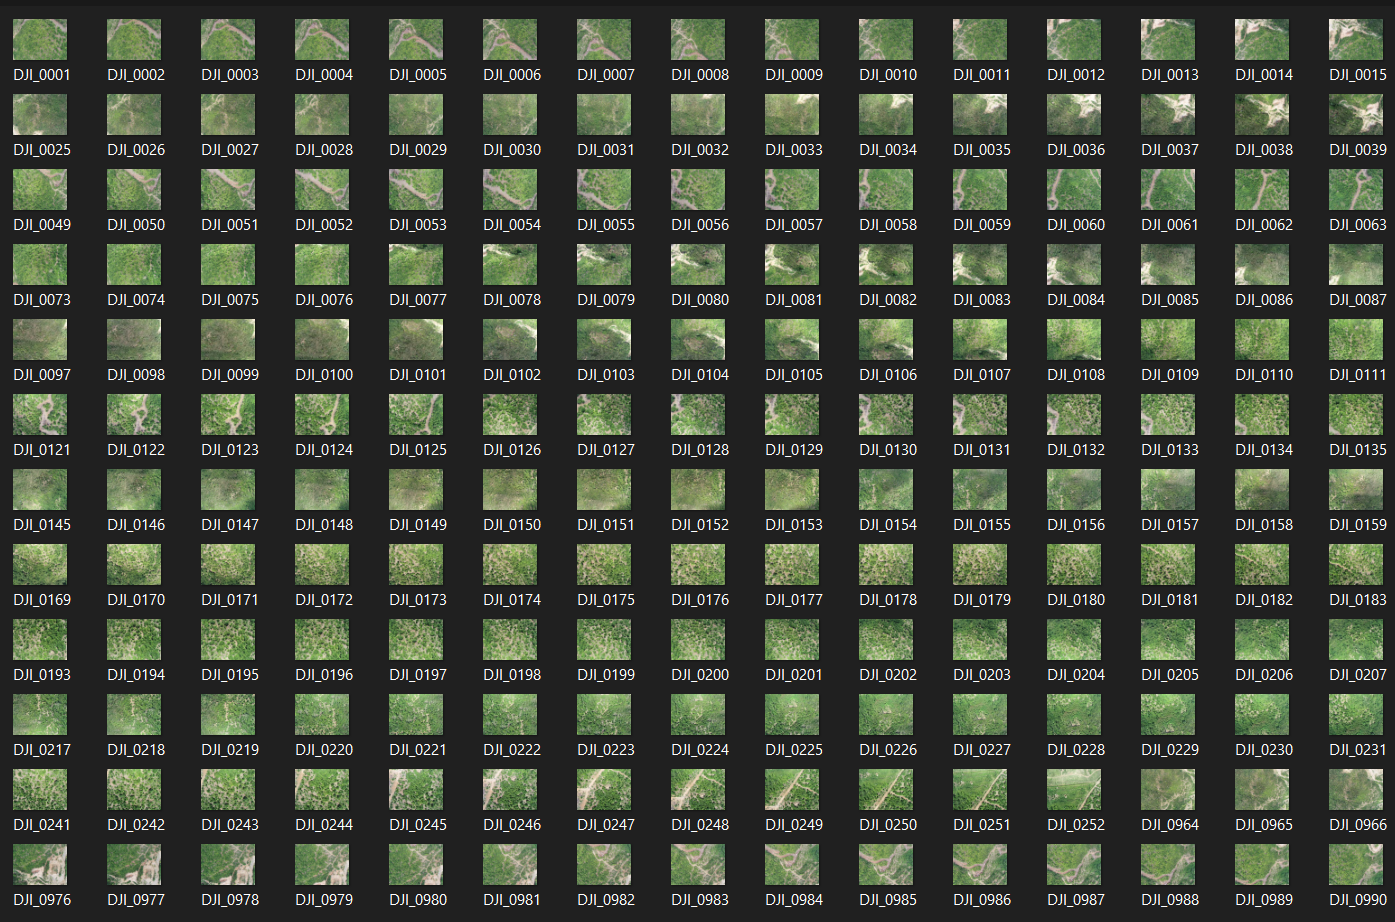
\includegraphics [width = 11.5cm,]{image/Kumpulan Citra}}
	\caption{Kumpulan citra udara yang digunakan dalam penelitian ini}
	\label{citra udara} % cuman gambar dummy ya !
\end{figure}

\begin{figure}[H]
        \centering
	\frame{\includegraphics [width = 11.5cm,]{image/DJI_0879}}
	\caption{Sampel foto Udara 1}
	\label{Sampel foto Udara 1} % cuman gambar dummy ya !
\end{figure}
\begin{figure}[H]
        \centering
	\frame{\includegraphics [width = 11.5cm,]{image/DJI_0880}}
	\caption{Sampel foto Udara 2}
	\label{Sampel foto Udara 2} % cuman gambar dummy ya !
\end{figure}
\begin{figure}[H]
        \centering
	\frame{\includegraphics [width = 11.5cm,]{image/DJI_0881}}
	\caption{Sampel foto Udara 3}
	\label{Sampel foto Udara 3} % cuman gambar dummy ya !
\end{figure}

\section{Metode Penelitian}

Analisis akuisisi data dan mosaik citra resolusi tinggi kawasan kampus II Universitas Syiah Kuala di Kecamatan Mesjid Raya, Aceh Besar dilakukan dengan beberapa tahapan, Gambar \ref{alur} dibawah ini memberikan informasi mengenai tahapan tersebut.

\begin{figure}[H]
	\centering
	{\includegraphics [width = 11.5cm,]{image/blank diagram.png}}
	\caption{Diagram alur penelitian}
	\label{alur} % cuman gambar dummy ya !
\end{figure}

\subsection{Studi Literatur}
Studi literatur dilakukan untuk memberikan dasar teoritis dan kontekstual bagi penelitian yang akan dilaksanakan. Proses ini melibatkan tinjauan yang mendalam terhadap kajian-kajian sebelumnya, jurnal ilmiah, buku, dan sumber-sumber lain yang relevan dengan topik penelitian. Analisis literatur membantu peneliti untuk memahami kemajuan pengetahuan terbaru, menganalisis pendekatan-pendekatan yang telah diambil oleh peneliti sebelumnya, serta mengidentifikasi kebutuhan solusi yang masih perlu dikembangkan. Analisis literatur juga membantu dalam menghindari duplikasi penelitian dan memastikan kontribusi penelitian baru terhadap literatur yang sudah ada.

\subsection{Analisis Akuisisi Data}
Akuisisi data citra di kawasan Kampus USK II, Kecamatan Mesjid Raya, Aceh Besar, dilakukan dengan menggunakan \textit{drone} DJI Phantom 4 Pro. Proses ini dimulai dengan perencanaan penerbangan \textit{drone} yang matang, meliputi penentuan area yang akan dipetakan, jalur penerbangan yang efisien, ketinggian terbang yang optimal, dan pengaturan \textit{overlap} antar citra yang diambil. Tahap selanjutnya adalah pengaturan kamera dan sensor yang terpasang pada \textit{drone} agar dapat menghasilkan kualitas citra yang baik, seperti resolusi gambar, laju pengambilan gambar, dan kemampuan sensor untuk menangkap informasi yang dibutuhkan. Pada tahap berikutnya, \textit{drone} melakukan penerbangan sesuai jalur yang telah direncanakan dan mengambil citra secara berangsur-angsur, merata, dan menyeluruh untuk mencakup seluruh kawasan lahan Kampus USK II. Proses ini membutuhkan ketelitian dan pemantauan yang cermat untuk memastikan tidak ada area yang terlewatkan dan tidak ada gangguan eksternal yang dapat mempengaruhi kualitas data. Setelah citra berhasil diambil, data tersebut ditransmisikan media penyimpanan yang sesuai dengan hati-hati untuk menghindari kehilangan atau kerusakan data. Setelah data berhasil disimpan, dilakukan verifikasi dan kontrol kualitas data yang meliputi pemeriksaan kelengkapan data, konsistensi resolusi dan kualitas citra, serta identifikasi adanya kesalahan atau noise yang dapat mempengaruhi analisis data. Langkah ini penting untuk memastikan bahwa data yang diperoleh memenuhi standar yang dibutuhkan untuk keperluan analisis selanjutnya. Analisis akuisisi data yang cermat dan terencana akan memastikan data citra yang diperoleh dari kawasan Kampus USK II memiliki kualitas yang baik dan dapat digunakan untuk berbagai keperluan, seperti pemantauan lingkungan, perencanaan infrastruktur, atau analisis tutupan lahan dan penggunaan lahan.

\subsection{Pengumpulan Data}
Dalam penelitian ini, proses pengumpulan data telah selesai dilaksanakan, dan penulis kini fokus pada pengorganisasian data ke dalam struktur folder yang sistematis untuk memudahkan analisis dan pemrosesan selanjutnya. Data yang diatur mencakup dua kategori utama yaitu serangkaian gambar hasil pemotretan menggunakan \textit{drone} dan data referensi lapangan berupa koordinat Ground Control Points (GCP) yang disimpan dalam format file teks. Citra-citra drone akan menjadi input utama dalam proses mosaik, sementara data GCP berperan krusial dalam meningkatkan akurasi geometrik dan georeferensi dari citra mosaik yang akan dihasilkan. Pengaturan data yang terstruktur ini tidak hanya akan memperlancar alur kerja pengolahan citra, tetapi juga akan mempermudah proses validasi  dan analisis akurasi spasial dari \textit{orthomosaic} yang dihasilkan. Selain itu, organisasi data yang baik akan memungkinkan perbandingan yang lebih efisien antara hasil pengolahan menggunakan Agisoft Metashape dan Pix4Dmapper, sesuai dengan tujuan penelitian untuk membandingkan kinerja kedua perangkat lunak tersebut.

\subsection{Mosaik}

Setelah berhasil mengumpulkan data citra dari seluruh wilayah penelitian di lahan Kampus 
USK II, langkah berikutnya adalah melakukan proses mosaik pada keseluruhan 
gambar. Hal ini bertujuan untuk menciptakan representasi visual menyeluruh dari 
kawasan yang telah diamati. Dalam penelitian ini, penulis melakukan proses mosaik 
pada citra menggunakan dua perangkat lunak berbeda, yakni Agisoft metashape dan PIX4Dmapper. 
Tujuan dari pendekatan ganda ini adalah untuk membandingkan hasil mosaik dari 
kedua perangkat lunak tersebut dan kemudian menyimpulkan manakah yang 
memberikan hasil yang lebih baik dan optimal dalam melakukan proses mosaik.

\subsection{Analisis Perbandingan}

\par Dalam penelitian ini, analisis komparatif berfokus pada tiga aspek utama yang dihasilkan oleh dua perangkat lunak fotogrametri, Agisoft Metashape dan Pix4Dmapper: akurasi geografis, resolusi spasial, dan efisiensi waktu pemrosesan. Evaluasi dilakukan dengan mempertimbangkan ground resolution dan resolusi orthomosaic yang dihasilkan oleh kedua perangkat lunak tersebut. Untuk menilai keakuratan geografis, akan dilakukan perbandingan menggunakan beberapa matriks evaluasi, termasuk \textit{Circular Error, Linear Error, dan Root Mean Square Error} (RMSE). Selain itu, penelitian ini akan mengukur dan membandingkan waktu yang dibutuhkan oleh masing-masing perangkat lunak untuk menyelesaikan proses pengolahan data. Terakhir, studi ini akan memverifikasi apakah hasil dari kedua perangkat lunak tersebut memenuhi standar ketelitian yang ditetapkan untuk peta Rupa Bumi Indonesia (RBI).


%-----------------------------------------------------------------------------%

% Baris ini digunakan untuk membantu dalam melakukan sitasi
% Karena diapit dengan comment, maka baris ini akan diabaikan
% oleh compiler LaTeX.
\begin{comment}
\bibliography{daftar-pustaka}
\end{comment}

\fancyhf{} 
\fancyfoot[R]{\thepage}

%-------------------------------------------------------------------------------
%                            BAB IV
%               		HASIL DAN PEMBAHASAN
%-------------------------------------------------------------------------------
% \fancyhf{} 
% \fancyfoot[R]{\thepage}
\chapter{HASIL DAN PEMBAHASAN}
%\thispagestyle{plain} % Halaman pertama bab menggunakan gaya plain

\section{Analisis akuisisi data}

Dalam penelitian ini, data citra udara hasil tangkapan drone beserta koordinat asli lapangan atau Ground Control Points (GCP) telah diakuisisi oleh staf ahli dari Laboratorium Terpadu Sistem Informasi Geografis dan Data Spasial Universitas Syiah Kuala. Fokus penelitian ini adalah analisis terhadap proses akuisisi data citra udara yang dihasilkan oleh drone. Berdasarkan analisis yang telah dilakukan, terdapat beberapa poin penting yang dapat diuraikan mengenai langkah-langkah akuisisi data tersebut.

\subsection{Desain jalur terbang \textit{drone}}

Dalam proses akuisisi data citra udara menggunakan drone, desain jalur terbang merupakan tahapan yang sangat krusial. Signifikansi desain ini terletak pada pengaruhnya terhadap kualitas citra yang dihasilkan dan efisiensi waktu yang diperlukan untuk menyelesaikan misi penerbangan. Beberapa aspek penting harus dipertimbangkan dalam merancang jalur terbang yang optimal. Pertama, perhitungan cermat mengenai daya tahan baterai sangat diperlukan untuk memastikan cakupan area yang direncanakan dapat terpenuhi dengan satu baterai penuh. Kedua, perencanaan rute harus mampu mencakup seluruh area target yang telah ditentukan sebelumnya. Ketiga, faktor lingkungan seperti arah angin merupakan elemen krusial yang harus diperhitungkan. Penerbangan melawan arah angin akan mengonsumsi daya lebih besar, sehingga dapat mempercepat habisnya baterai selama proses akuisisi data. Dengan mempertimbangkan faktor-faktor tersebut, desain jalur terbang yang optimal dapat menghasilkan citra berkualitas tinggi sekaligus mengoptimalkan penggunaan sumber daya drone, terutama dalam hal konsumsi baterai dan waktu penerbangan.

Dalam proses akuisisi data lahan Kampus II Universitas Syiah Kuala, perencanaan jalur terbang didesain menggunakan perangkat lunak Drone Deploy. Aplikasi ini memungkinkan pengaturan area yang akan dilewati drone, konfigurasi bentuk jalur terbang, serta penyesuaian front overlap dan side overlap antar foto. Selain itu, perangkat lunak ini juga menyediakan estimasi waktu penerbangan dan penggunaan daya baterai drone untuk setiap misi. Penulis telah melakukan analisis perbandingan antara jalur terbang dominan vertikal dan dominan horizontal untuk menentukan efisiensi waktu dan penggunaan daya. Kedua jalur terbang ini dapat dilihat pada Gambar \ref{jalur terbang 1} dan \ref{jalur terbang 2}, sementara perbandingan detailnya disajikan dalam Tabel \ref{tab:perbandingan_jalur}.

\begin{figure}[H]
    \centering
    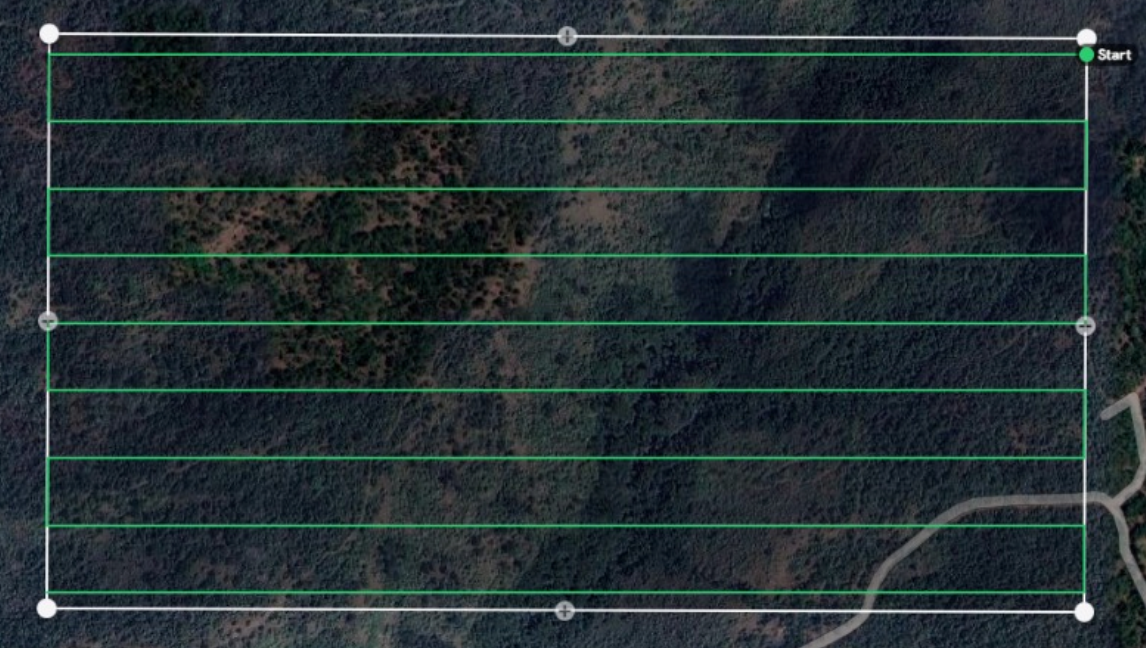
\includegraphics[width = 11.5cm]{image/desain jalur terbang 1.PNG}
    \caption{Jalur terbang dominan horizontal}
    \label{jalur terbang 1}
\end{figure}

\begin{figure}[H]
    \centering
    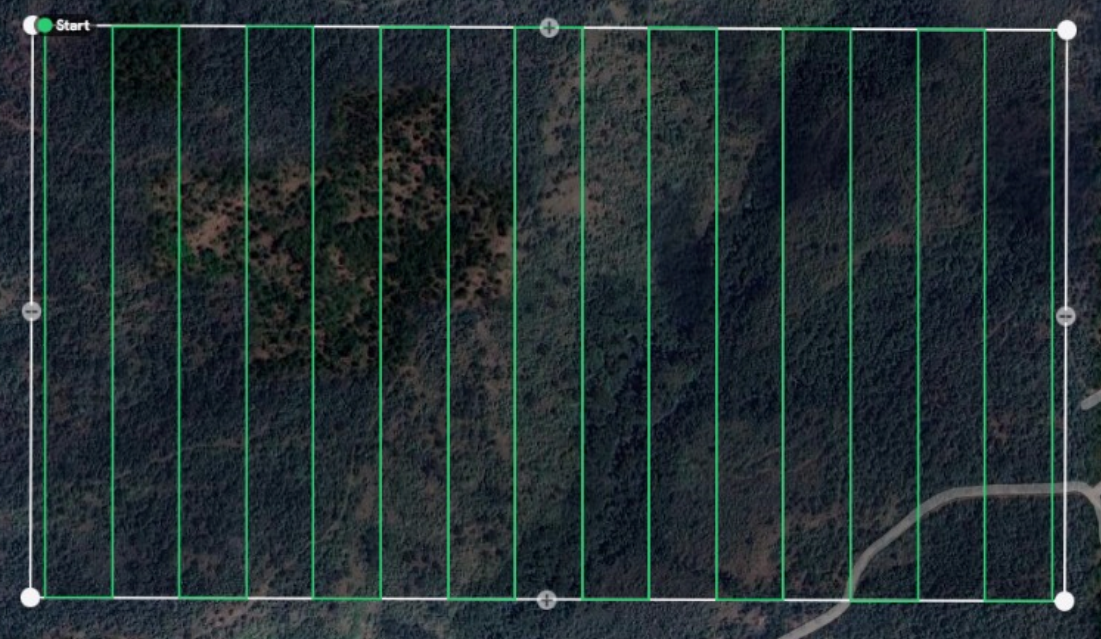
\includegraphics[width = 11.5cm]{image/desain jalur terbang 2.PNG}
    \caption{Jalur terbang dominan vertikal}
    \label{jalur terbang 2}
\end{figure}

\begin{table}[h]
\centering
\caption{Perbandingan jalur terbang dominan vertikal dan horizontal}
\begin{tabular}{|c|c|c|c|c|c|c|}
\hline
\textbf{No} & \textbf{\begin{tabular}[c]{@{}c@{}}Jalur\\terbang\end{tabular}} & \textbf{\begin{tabular}[c]{@{}c@{}}Luas\\Area (H)\end{tabular}} & \textbf{\begin{tabular}[c]{@{}c@{}}Jumlah\\Gambar\end{tabular}} & \textbf{\begin{tabular}[c]{@{}c@{}}Kecepatan\\terbang\\(m/s)\end{tabular}} & \textbf{Baterai} & \textbf{\begin{tabular}[c]{@{}c@{}}Waktu\\(menit)\end{tabular}} \\
\hline
1 & \begin{tabular}[c]{@{}c@{}}Dominan\\Vertikal\end{tabular} & 55 & 283 & 12 & 2 & 18:20 \\
\hline
2 & \begin{tabular}[c]{@{}c@{}}Dominan\\Horizontal\end{tabular} & 55 & 288 & 12 & 2 & 16:46 \\
\hline
\end{tabular}
\label{tab:perbandingan_jalur}
\end{table}

Berdasarkan hasil analisis yang disajikan dalam Tabel \ref{tab:perbandingan_jalur}, dapat ditarik beberapa kesimpulan penting. Pertama, jalur terbang dominan horizontal menunjukkan efisiensi yang lebih tinggi dibandingkan dengan jalur dominan vertikal. Hal ini tercermin dari kemampuannya untuk mengambil jumlah gambar yang lebih banyak (288 dibandingkan 283) dalam waktu yang lebih singkat (16:46 menit berbanding 18:20 menit). Selain itu, analisis ini juga mengungkapkan korelasi antara frekuensi belokan drone dengan durasi misi. Semakin sering drone harus berbelok untuk mencapai jalur pengambilan foto utama, semakin lama waktu yang dibutuhkan untuk menyelesaikan pemetaan area tersebut. Hal ini menjelaskan mengapa jalur dominan horizontal, yang umumnya memiliki lebih sedikit belokan, dapat menyelesaikan misi dengan lebih cepat. Temuan-temuan ini memberikan wawasan berharga untuk optimalisasi perencanaan jalur terbang drone dalam misi pemetaan, dengan implikasi signifikan terhadap efisiensi waktu dan produktivitas pengambilan data.

\subsection{ketinggian dan kecepatan terbang}

Penelitian ini dilakukan di lahan Kampus II Universitas Syiah Kuala, tepatnya di Kecamatan Mesjid Raya, Kabupaten Aceh Besar. Karakteristik area penelitian berupa perbukitan dengan vegetasi lebat, yang menjadi tantangan tersendiri dalam melakukan pemetaan menggunakan drone. Dalam konteks pemetaan drone, ketinggian terbang merupakan faktor krusial yang harus dipertimbangkan dengan cermat. Terdapat hubungan berbanding terbalik antara ketinggian terbang dengan detail dan cakupan area foto, semakin rendah drone terbang, semakin tinggi detail yang dapat ditangkap oleh kamera drone, namun semakin sempit area yang tercakup dalam sebuah foto. Sebaliknya, semakin tinggi ketinggian terbang drone, semakin rendah detail yang dapat ditampilkan, tetapi semakin luas area yang dapat dicakup dalam satu foto. Untuk penelitian ini, ketinggian terbang drone ditetapkan pada 150 meter di atas permukaan tanah, menyeimbangkan kebutuhan detail dan cakupan area.

Selain ketinggian, kecepatan terbang drone juga merupakan parameter penting yang perlu dioptimalkan saat pengambilan foto udara. Kecepatan drone tidak hanya mempengaruhi durasi misi, tetapi juga berdampak signifikan terhadap kualitas gambar yang dihasilkan. Dalam kondisi pencahayaan rendah, drone perlu bergerak lebih lambat untuk menghasilkan gambar yang detail. Hal ini disebabkan oleh penyesuaian shutter speed kamera drone terhadap kondisi cahaya yang minim, mengakibatkan proses pengambilan foto menjadi lebih lambat. Jika drone bergerak terlalu cepat dalam kondisi ini, hasil foto cenderung akan terlihat blur. Sebaliknya, dalam kondisi pencahayaan yang optimal, seperti pada siang hari, drone dapat bergerak lebih cepat. Hal ini dimungkinkan karena shutter speed kamera drone dapat bekerja lebih efisien berkat cahaya yang cukup, sehingga mampu menghasilkan gambar yang tetap tajam dan minim blur meskipun pada kecepatan tinggi. Dalam penelitian ini, proses akuisisi data dilaksanakan pada siang hari dengan kondisi pencahayaan yang optimal. Oleh karena itu, kecepatan terbang drone dapat diatur lebih tinggi, yaitu pada 12 m/s, yang terbukti mampu menghasilkan gambar dengan ketajaman dan detail yang sangat baik.

\subsection{overlapping}

Dalam proses akuisisi data citra resolusi tinggi di kawasan Kampus II Universitas Syiah Kuala, penelitian ini menggunakan komposisi front overlap sebesar 75\% dan side overlap 65\%. Pengaturan ini berada dalam rentang optimal untuk pemetaan fotogrametri menggunakan drone, memastikan kontinuitas data spasial dan memungkinkan rekonstruksi 3D yang akurat. Pemilihan nilai overlapping ini didasarkan pada beberapa pertimbangan, termasuk karakteristik terrain kampus yang beragam dengan area berbukit dan bervegetasi lebat, kebutuhan akan akurasi data tinggi, kompensasi terhadap potensi ketidakstabilan drone akibat faktor lingkungan, serta keseimbangan antara kualitas data dan efisiensi operasional.

Meskipun pengaturan ini terbukti efektif untuk sebagian besar area kampus, beberapa tantangan ditemui di zona dengan vegetasi sangat rapat, menunjukkan perlunya pertimbangan untuk meningkatkan overlap di area-area khusus pada penelitian mendatang. Secara keseluruhan, penggunaan front overlap 75\% dan side overlap 65\% terbukti efektif dalam menghasilkan data spasial yang detail dan akurat, memenuhi tujuan pemetaan kawasan Kampus II Universitas Syiah Kuala.

\subsection{Pengambilan \textit{Ground Control Point} (GCP)}

Proses akuisisi data Ground Control Point (GCP) dalam penelitian ini dilakukan menggunakan GPS Geodetik Hi-Target, yang dikenal dengan akurasinya yang tinggi. Sejumlah 16 titik GCP ditetapkan, yang dikategorikan sebagai 3D GCP karena mencakup data longitude, latitude, dan altitude, memberikan referensi spasial yang komprehensif untuk studi kasus area seluas 250 hektar. Strategi penempatan GCP dirancang dengan cermat, dengan satu titik GCP ditempatkan untuk setiap misi penerbangan drone, memastikan cakupan yang merata dan representatif di seluruh area penelitian. Untuk memudahkan identifikasi GCP dalam citra udara, setiap titik ditandai di lapangan menggunakan terpal berwarna merah berbentuk X, seperti yang diilustrasikan pada Gambar 4.4. Pemilihan lokasi GCP dilakukan dengan pertimbangan khusus, dengan preferensi pada area terbuka yang minim vegetasi untuk memaksimalkan visibilitas dan meminimalkan potensi gangguan sinyal GPS. Penempatan strategis ini tidak hanya memfasilitasi deteksi yang akurat dalam citra drone tetapi juga memastikan kualitas sinyal GPS yang optimal selama pengukuran.

Selain proses pengambilan, data GCP sangat penting dalam proses pembuatan peta yang akurat. GCP berfungsi seperti titik-titik acuan yang lokasinya diketahui dengan pasti di lapangan. Cara kerjanya adalah dengan membandingkan lokasi GCP yang diukur di lapangan menggunakan GPS akurat, dengan lokasi yang sama yang terlihat di foto drone. Melalui perbandingan ini, posisi dan bentuk foto-foto drone dapat diperbaiki agar sesuai dengan kenyataan di lapangan. Proses ini disebut georeferensi dan ortorektifikasi. Hasilnya adalah sebuah peta foto (orthomosaic) yang tidak hanya terlihat bagus, tapi juga akurat secara posisi. Keakuratan ini sangat penting karena membuat peta dapat digunakan bersama dengan data-data peta lainnya tanpa ada masalah perbedaan posisi. Misalnya, peta ini dapat digabungkan dengan peta jalan atau peta bangunan yang sudah ada sebelumnya.

\section{Pengumpulan Data}

Dalam penelitian ini, penulis tidak melakukan akuisisi data foto udara lahan Kampus II Universitas Syiah Kuala secara langsung. Hal ini dikarenakan data foto udara dan data pendukung spasial lainnya telah disediakan dan diakuisisi sebelumnya oleh staf Laboratorium Sistem Informasi Geografis dan Data Spasial Universitas Syiah Kuala. Peran penulis dalam tahap ini terbatas pada pengumpulan dan penyusunan data yang diberikan ke dalam struktur folder yang sistematis, guna memudahkan proses pengolahan dan mosaik di tahap selanjutnya. Dataset yang diperoleh terdiri dari 4.701 foto udara hasil tangkapan drone DJI Phantom 4 Pro. Selain itu, data pendukung spasial lainnya juga disertakan, meliputi data koordinat 3D Ground Control Points (GCP) dalam format XYZ, serta data batas administrasi lahan Kampus II USK dan area studi penelitian. Untuk memberikan gambaran visual, contoh hasil tangkapan drone dapat dilihat pada Gambar \ref{pengda}, sementara data GCP disajikan dalam Tabel \ref{tab:gcp_data}.

\begin{figure} [H]
    \centering
    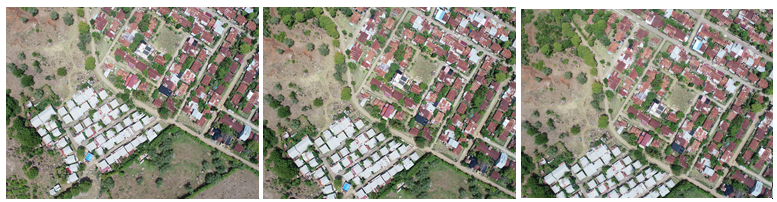
\includegraphics[width=1\linewidth]{image/data.png}
    \caption{Data foto udara \textit{drone}}
    \label{pengda}
\end{figure}

\begin{table} [H]
\centering
\caption{Data Ground Control Point (GCP) area studi penelitian}
\begin{tabular}{|c|c|c|c|}
\hline
\textbf{Label} & \textbf{Latitude} & \textbf{Longitude} & \textbf{Altitude} \\
\hline
GCP 1 & 5.645281 & 95.42608 & 54.587 \\
GCP 2 & 5.646212 & 95.43401 & 38.432 \\
GCP 3 & 5.646481 & 95.44335 & 9.51 \\
GCP 4 & 5.641528 & 95.43029 & 134.79 \\
GCP 5 & 5.641895 & 95.44016 & 94.559 \\
GCP 6 & 5.642268 & 95.44834 & 24.766 \\
GCP 7 & 5.638084 & 95.42901 & 172.052 \\
GCP 8 & 5.63729 & 95.44009 & 185.723 \\
GCP 9 & 5.636904 & 95.44481 & 160.798 \\
GCP 10 & 5.633782 & 95.42898 & 173.878 \\
GCP 11 & 5.633573 & 95.44081 & 180.413 \\
GCP 12 & 5.633305 & 95.44552 & 167.8 \\
GCP 13 & 5.629193 & 95.43453 & 259.766 \\
GCP 14 & 5.630646 & 95.44323 & 245.943 \\
GCP 15 & 5.626161 & 95.43446 & 265.061 \\
GCP 16 & 5.625719 & 95.44308 & 313.595 \\
\hline
\end{tabular}
\label{tab:gcp_data}
\end{table}

\par Dalam proses pengumpulan data, penulis mengadopsi metode pengorganisasian yang sistematis untuk foto-foto udara. Setiap misi penerbangan drone, yang berjumlah total 16 kali di area studi, direpresentasikan oleh satu folder terpisah. Pendekatan ini memungkinkan penulis untuk dengan mudah mengidentifikasi dan menghitung jumlah foto yang diambil dalam setiap misi penerbangan spesifik. Struktur penyimpanan yang terorganisir ini tidak hanya meningkatkan efisiensi dalam pengelolaan dan analisis data visual, tetapi juga meminimalisir risiko kesalahan dalam pengolahan data. Lebih lanjut, metode ini sangat bermanfaat dalam menghadapi potensi tantangan teknis, seperti memudahkan identifikasi dan isolasi masalah jika terjadi error pada area tertentu. Dengan demikian, penulis dapat dengan cepat menavigasi dan mengelola dataset yang besar, sambil mempertahankan integritas data untuk setiap misi penerbangan, yang sangat penting dalam menjaga kualitas hasil penelitian. detail pembagian folder dan jumlah foto pada setiap misi penerbangan dapat dilihat pada tabel \ref{tab:folder}

\begin{table} [H]
\centering
\caption{Pembagian folder dan detail jumlah foto udara didalamnya}
\begin{tabular}{|l|c|}
\hline
\textbf{Nama Folder} & \textbf{Jumlah Foto Udara} \\ \hline
Folder 1 & 291 \\ \hline
Folder 2 & 295 \\ \hline
Folder 3 & 292 \\ \hline
Folder 4 & 291 \\ \hline
Folder 5 & 297 \\ \hline
Folder 6 & 294 \\ \hline
Folder 7 & 293 \\ \hline
Folder 8 & 293 \\ \hline
Folder 9 & 288 \\ \hline
Folder 10 & 292 \\ \hline
Folder 11 & 296 \\ \hline
Folder 12 & 321 \\ \hline
Folder 13 & 285 \\ \hline
Folder 14 & 291 \\ \hline
Folder 15 & 287 \\ \hline
Folder 16 & 296 \\ \hline
\textbf{Total} & \textbf{4701} \\ \hline
\end{tabular}
\label{tab:folder}
\end{table}

\section{mosaik}

\par Pada tahap mosaik ini, penulis akan melakukan proses mosaik menggunakan dua perangkat lunak yang berbeda, yaitu Agisoft Metashape dan Pix4Dmapper. Tujuan dari penggunaan dua perangkat lunak yang berbeda ini adalah untuk membandingkan hasilnya dan menentukan mana yang akan menghasilkan akurasi dan resolusi yang lebih baik.

\subsection{Agisoft Metashape}

\par Dalam penelitian ini, proses mosaik menggunakan perangkat lunak Agisoft Metashape melibatkan beberapa tahap pemrosesan, yaitu align photo, build point cloud, build model, build texture, build DEM, dan build orthomosaic. Langkah pertama yang harus dilakukan adalah mengimpor seluruh foto udara ke dalam perangkat lunak Agisoft Metashape. Penting untuk memastikan bahwa semua foto udara telah dimasukkan dengan lengkap, tanpa ada satu pun yang tertinggal. Align Photo merupakan tahap awal yang krusial dalam proses menghasilkan orthomosaik dari foto udara yang diambil menggunakan drone. Pada tahap ini, perangkat lunak Agisoft Metashape akan memposisikan foto-foto berdasarkan data koordinat yang terekam saat drone melakukan pemotretan udara. Selain menempatkan foto sesuai dengan data koordinat, perangkat lunak juga mengidentifikasi sudut pengambilan gambar drone terhadap permukaan lahan yang dipotret. Penting untuk memastikan bahwa semua foto telah diatur dengan tepat sebelum melanjutkan ke tahap berikutnya. Hasil dari proses ini berupa titik-titik informasi relatif dari setiap foto dalam ruang tiga dimensi yang dapat dilihat pada Gambar \ref{tiepoint}, yang menjadi dasar untuk tahap-tahap selanjutnya dalam pembuatan orthomosaik.

\begin{figure} [H]
    \centering
    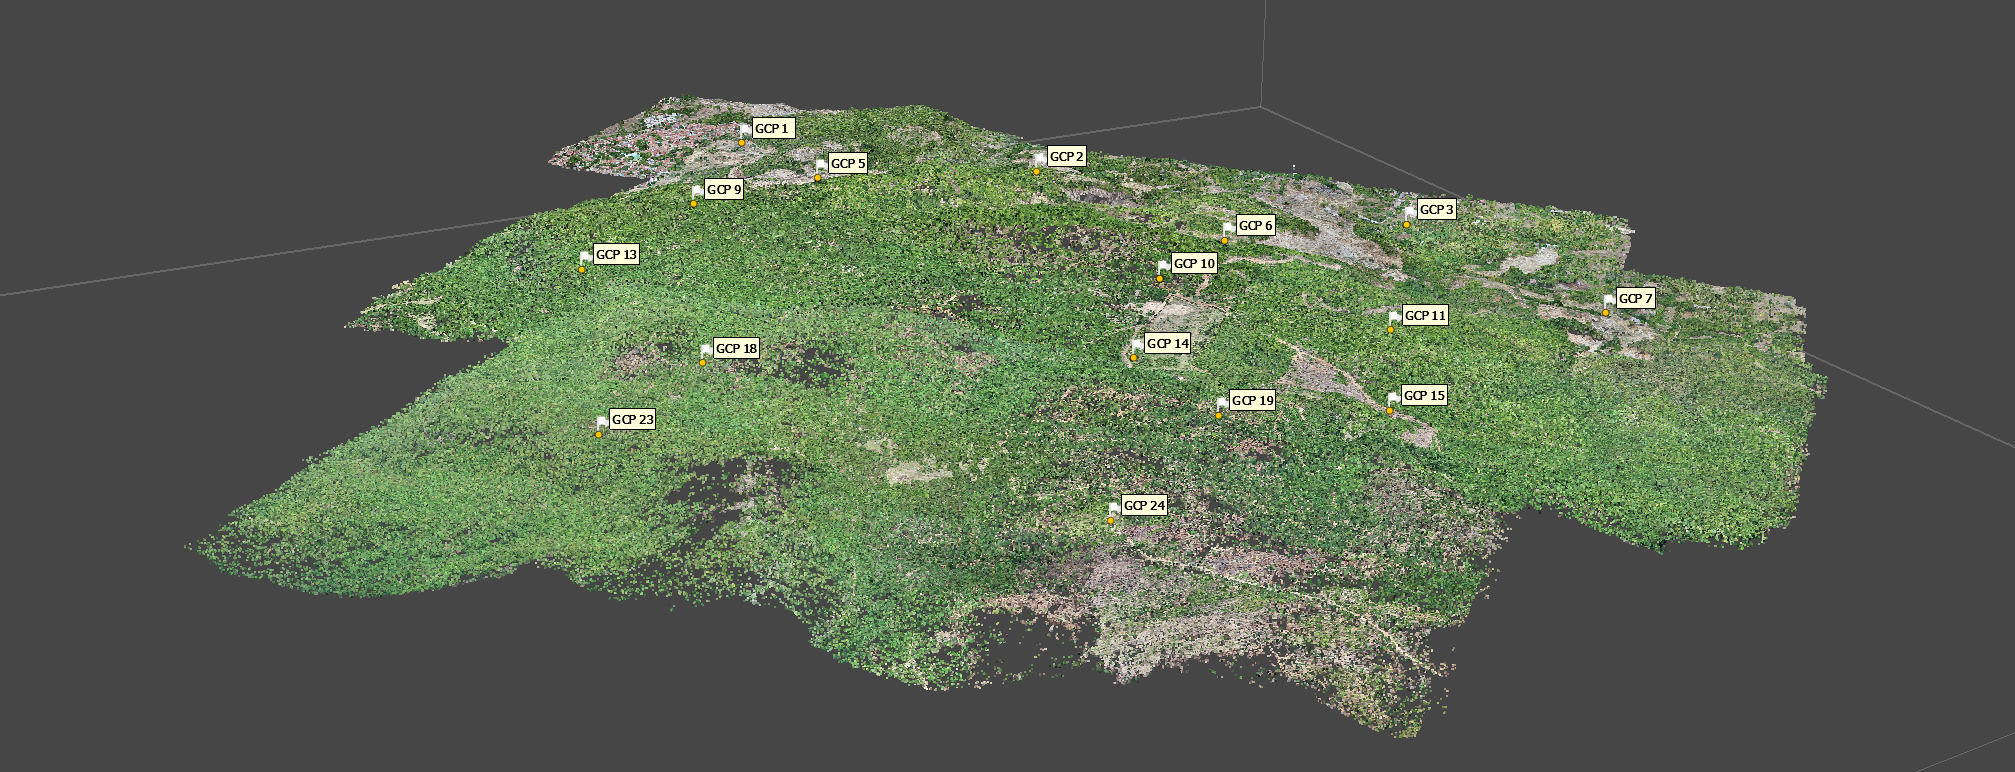
\includegraphics[width=1\linewidth]{image/Tie Point.png}
    \caption{Hasil output dari proses align photo}
    \label{tiepoint}
\end{figure}

Setelah tahap Align Photo berhasil dilaksanakan, langkah berikutnya dalam pemetaan lahan menggunakan drone adalah memasukkan dan menyesuaikan titik Ground Control Point (GCP). Proses ini melibatkan penyelarasan antara koordinat GCP dengan titik-titik yang telah ditandai pada citra hasil tangkapan drone. Dalam penelitian ini, penanda GCP berupa terpal merah berbentuk X digunakan sebagai referensi, seperti yang terlihat pada Gambar \ref{terpal merah}.

\begin{figure} [H]
    \centering
    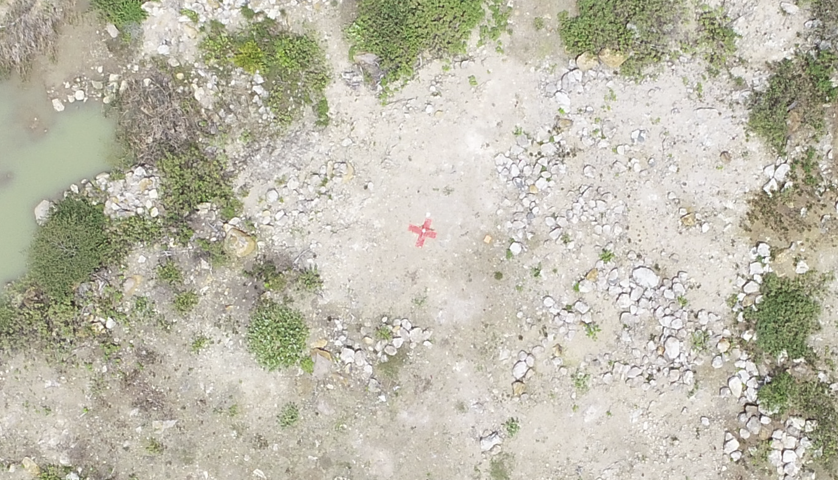
\includegraphics[width = 11.5cm]{image/tanda GCP di lapangan.png}
    \caption{Terpal merah sebagai titik penanda di lapangan}
    \label{terpal merah}
\end{figure}

Penyesuaian koordinat GCP dilakukan dengan teliti pada beberapa citra yang memuat penanda GCP. Berdasarkan tahap pengumpulan data sebelumnya, dataset citra dibagi menjadi 16 folder, masing-masing berisi sekitar 290 gambar dan memiliki satu GCP yang telah ditentukan. Dengan demikian, total GCP yang digunakan dalam proyek ini berjumlah 16 titik. Distribusi spasial dari titik-titik GCP dapat dilihat pada Gambar \ref{penyebaran}. Sementara itu, tahapan penyesuaian koordinat GCP terhadap citra drone diilustrasikan pada Gambar \ref{gcptidakakurat} dan \ref{gcpakurat}, memberikan gambaran visual tentang proses penyelarasan yang dilakukan.

\begin{figure} [H]
    \centering
    \frame{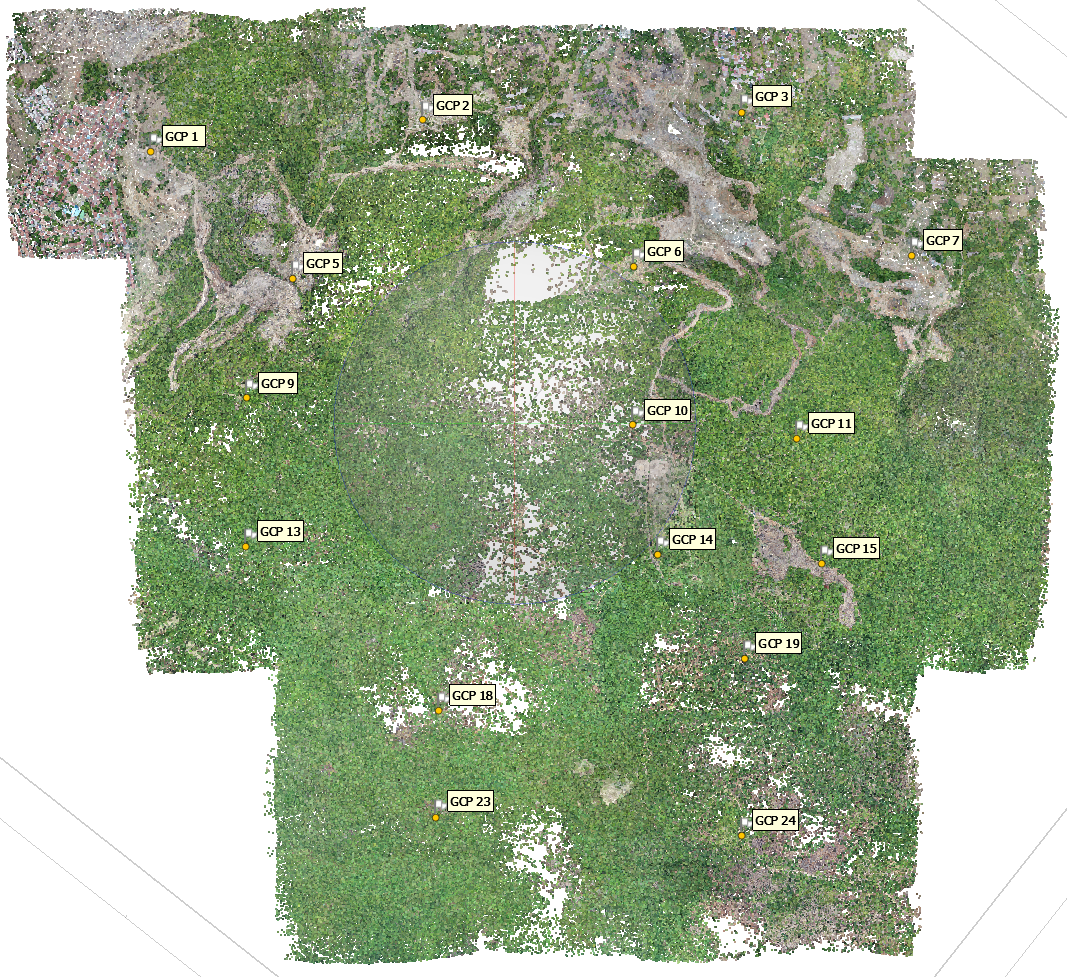
\includegraphics[width=1\linewidth]{image/penyebaran titik GCP - setelah align photo.png}}
    \caption{Penyebaran titik Ground Control Point di area penelitian}
    \label{penyebaran}
\end{figure}

\begin{figure}[H]
    \centering
    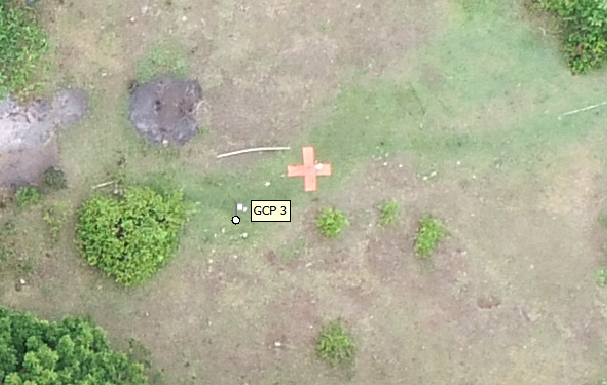
\includegraphics[width = 11.5cm]{image/gcp tidak akurat.png}
    \caption{Titik Ground Control Point sebelum di koreksi}
    \label{gcptidakakurat}
\end{figure}

\begin{figure}[H]
    \centering
    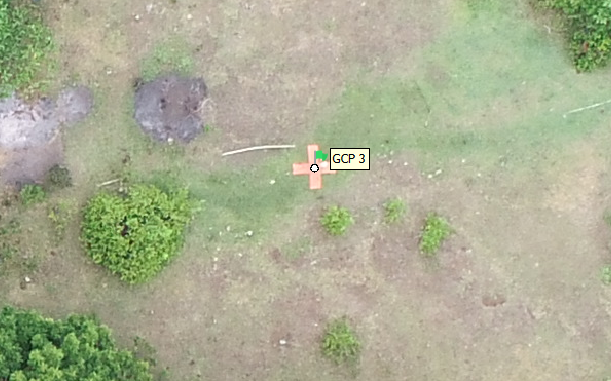
\includegraphics[width = 11.5cm]{image/gcp akurat.png}
    \caption{Titik Ground Control Point setelah di koreksi}
    \label{gcpakurat}
\end{figure}


Tahap selanjutnya adalah Build Point Cloud, sebuah proses yang memerlukan waktu lebih lama dan sumber daya perangkat keras yang paling intensif. Dalam tahap ini, perangkat lunak Agisoft Metashape menghasilkan titik-titik 3D yang secara akurat merepresentasikan permukaan objek atau area lahan yang dipetakan. Perangkat lunak ini memanfaatkan informasi yang diperoleh dari foto-foto yang telah diatur sebelumnya untuk menentukan posisi 3D dari fitur-fitur yang terlihat pada setiap gambar dengan presisi tinggi. Hasil dari proses ini adalah kumpulan titik-titik yang mewakili struktur permukaan yang dipetakan, dengan tingkat kepadatan yang jauh lebih tinggi dibandingkan tie points yang dihasilkan pada tahap Align Photo. Dalam penelitian ini, proses Build Point Cloud memakan waktu 13 jam 48 menit dengan pengaturan kualitas tinggi (High Quality), menghasilkan 1.850.290.607 titik. Visualisasi hasil dari tahap Build Point Cloud dapat dilihat pada Gambar \ref{point cloude}.

\begin{figure} [H]
    \centering
    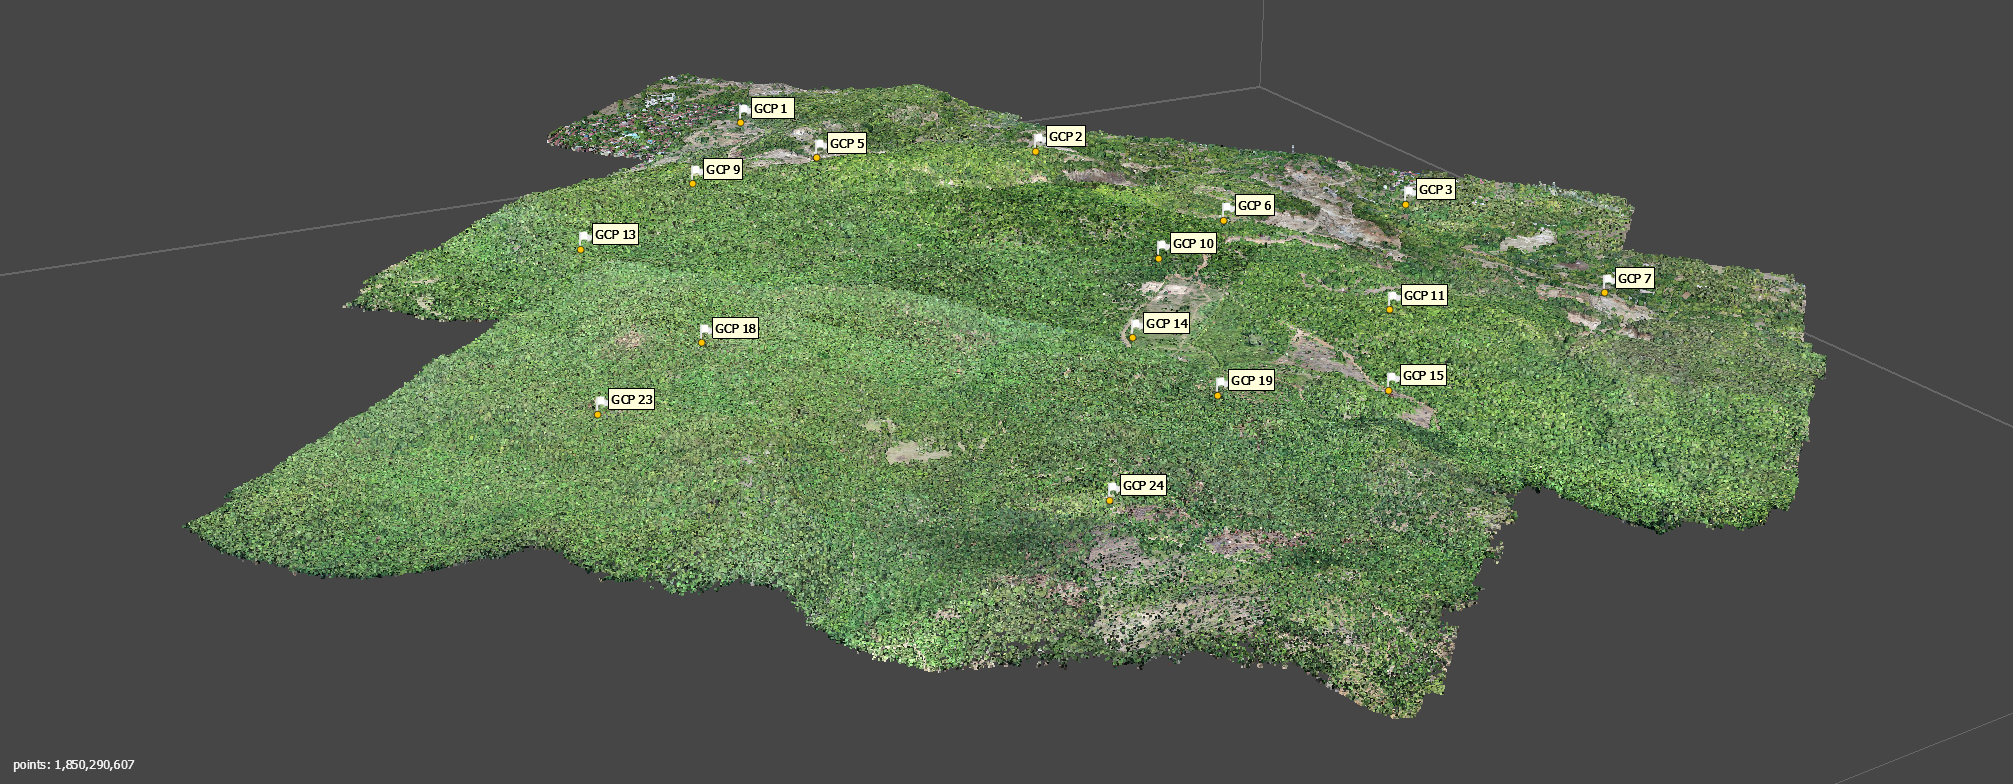
\includegraphics[width=1\linewidth]{image/point cloude.png}
    \caption{Hasil output dari proses build point cloud}
    \label{point cloude}
\end{figure}

\par Setelah point cloud terbentuk, langkah berikutnya adalah membangun model 3D beserta teksturnya. Dalam perangkat lunak Agisoft Metashape, proses ini dapat dijalankan secara terpisah melalui dua tahap yaitu Build Model dan Build Texture. Tahap Build Model menghasilkan model 3D yang solid dan representatif dari objek atau area yang dipetakan. Proses ini menghubungkan titik-titik dari point cloud untuk membentuk permukaan yang mulus dan menghasilkan representasi 3D yang akurat. Hasilnya adalah model 3D yang dapat dilihat dan dimanipulasi. Untuk memperoleh hasil visual yang menarik dan detail yang lebih baik, proses Build Mesh harus dipadukan dengan tahap Build Texture. Pada tahap ini, Agisoft Metashape memetakan kembali gambar-gambar asli dari setiap sudut pengambilan foto ke model 3D. Hasilnya adalah model yang memiliki penampilan realistis dengan warna dan tekstur yang sesuai dengan objek sebenarnya, memberikan visualisasi yang lebih detail dan nyata dari struktur atau area yang dipetakan. Hasil akhir dari proses Build Model dan Build Texture dapat dilihat pada Gambar \ref{model3d}, menampilkan model 3D bertekstur yang menggambarkan area pemetaan dengan tingkat detail dan realisme yang tinggi.

\begin{figure} [H]
    \centering
    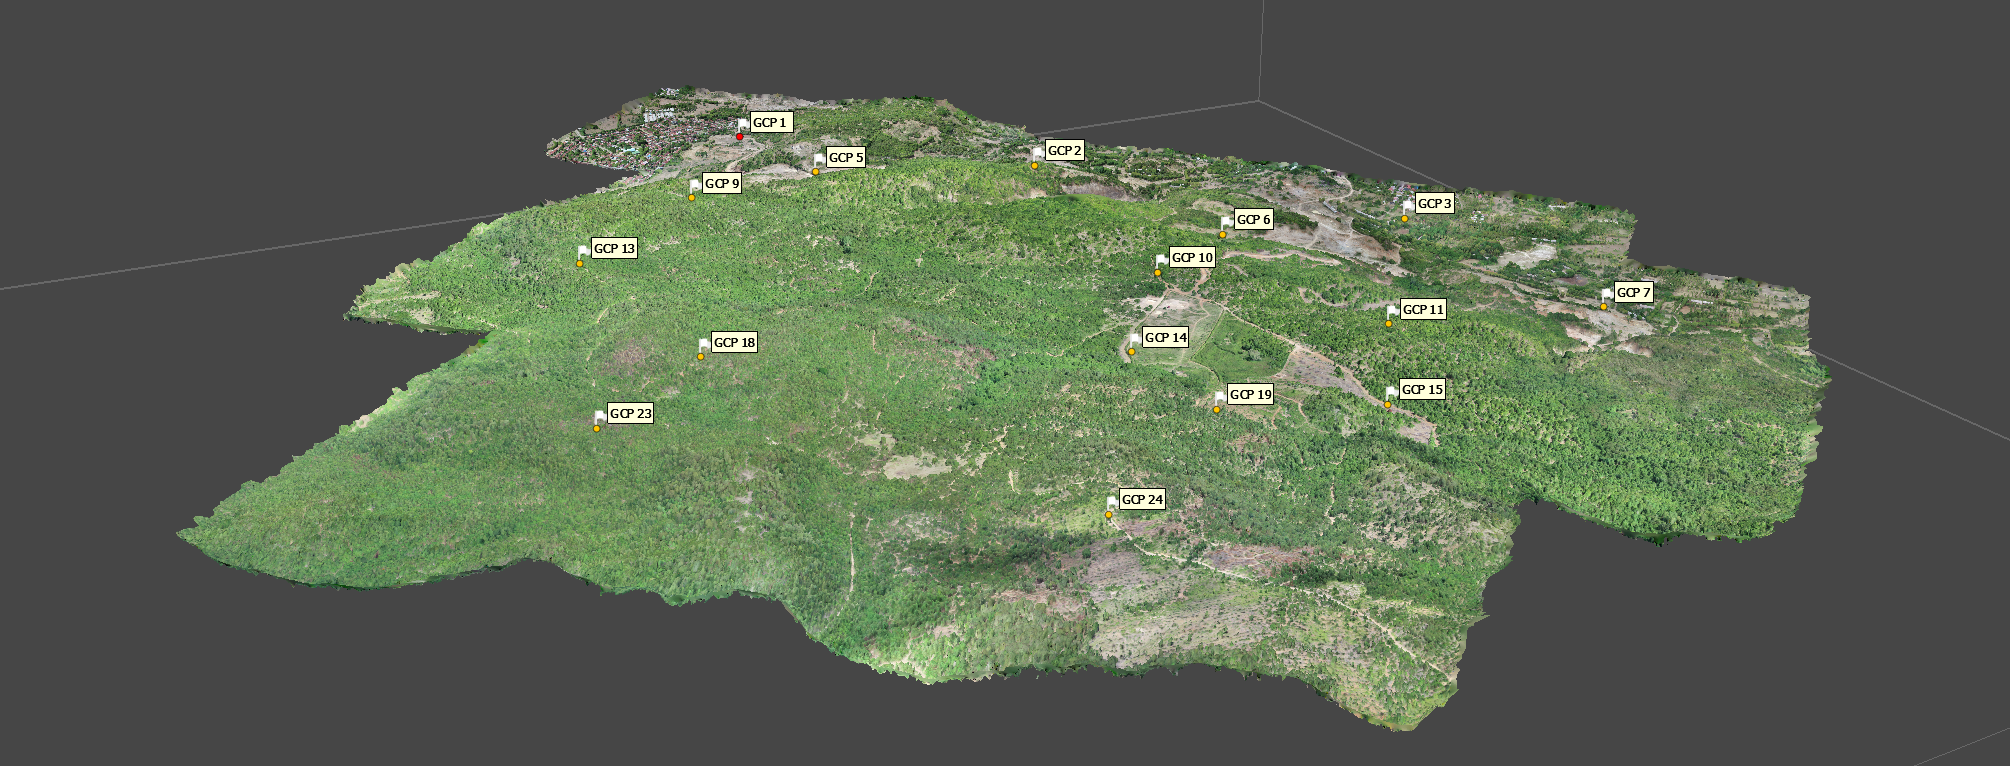
\includegraphics[width=1\linewidth]{image/Tampilan 3d model.png}
    \caption{Hsil output dari proses build model dan build texture}
    \label{model3d}
\end{figure}

\par Setelah proses Build Mesh dan Build Texture berhasil dilaksanakan, langkah selanjutnya adalah membangun Digital Elevation Model (DEM). Tahap ini merupakan proses yang relatif cepat, bahkan dapat selesai dalam hitungan menit. Pada tahap ini, perangkat lunak Agisoft Metashape memanfaatkan data yang telah diolah sebelumnya untuk menghasilkan model digital yang merepresentasikan elevasi permukaan tanah atau objek di area yang dipetakan. DEM yang dihasilkan oleh Agisoft Metashape merupakan output 2D. DEM ini adalah representasi raster dari elevasi permukaan bumi, di mana setiap piksel menyimpan nilai ketinggian tertentu. Meskipun outputnya 2D, DEM ini mampu menggambarkan informasi ketinggian dalam bentuk yang dapat diinterpretasikan sebagai relief permukaan. Output DEM ini biasanya ditampilkan dengan gradasi warna atau bayangan (hillshade) untuk memvisualisasikan perbedaan elevasi. Warna-warna yang berbeda atau intensitas bayangan menunjukkan variasi ketinggian di seluruh area yang dipetakan.

Hasil dari proses Build DEM ini dapat dilihat pada Gambar \ref{dem}, yang menampilkan peta elevasi 2D dari area yang dipetakan, dengan skema warna yang menunjukkan perbedaan ketinggian.
DEM 2D ini tetap sangat berguna untuk berbagai analisis seperti perhitungan kemiringan, aspek, dan kontur, serta dapat digunakan sebagai input untuk analisis perencanaan lahan, dan aplikasi GIS lainnya.

\begin{figure} [H]
    \centering
    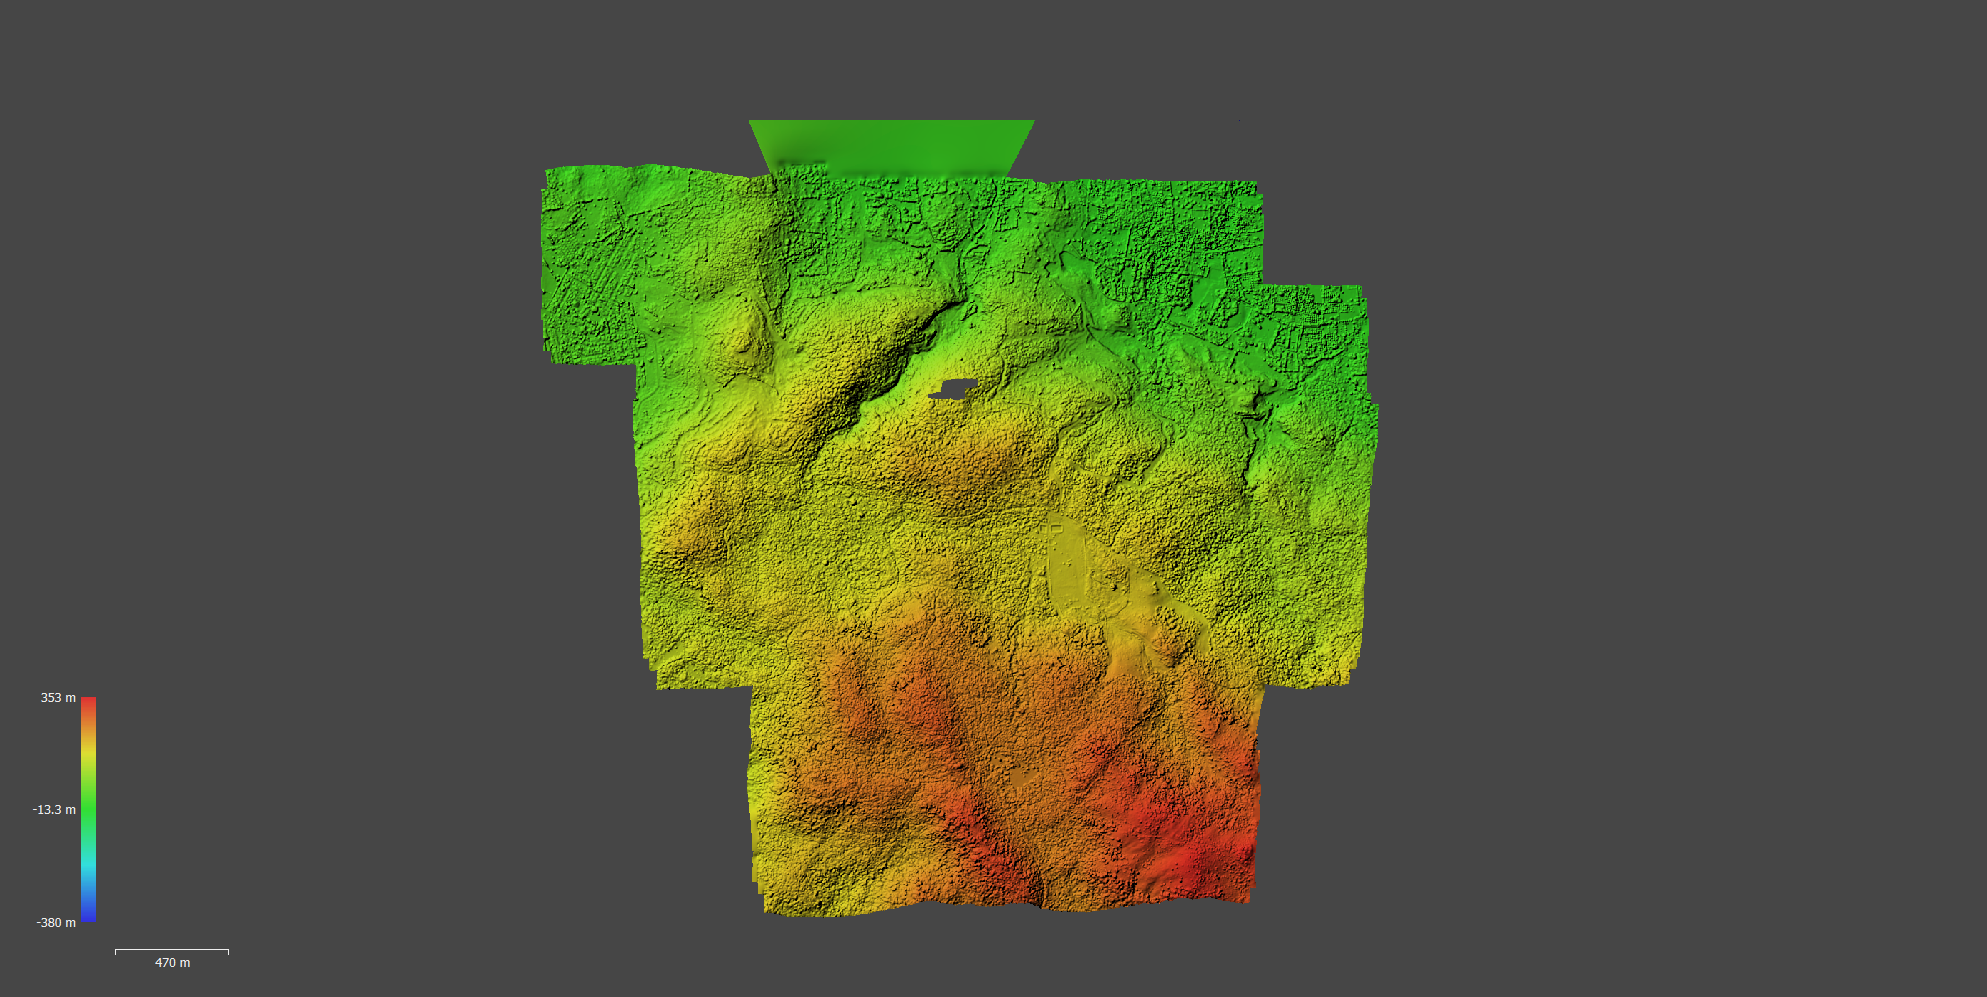
\includegraphics[width=1\linewidth]{image/DEM.png}
    \caption{Hasil output dari proses build Digital Elevation Model (DEM)}
    \label{dem}
\end{figure}

\par Setelah proses Build DEM selesai, tahap terakhir yang dilakukan adalah Build Orthomosaic. Pada tahap ini, perangkat lunak Agisoft Metashape akan menghasilkan ortofoto, yang merupakan citra udara yang telah dikoreksi secara geometris dari area yang dipetakan. Proses ini menggabungkan informasi dari seluruh foto yang telah diatur sebelumnya untuk menciptakan representasi visual yang akurat secara geometris dari wilayah yang diteliti. Hasil akhir dari proses ini adalah orthomosaik, yaitu citra yang memiliki presisi tinggi dari area penelitian, seperti yang ditunjukkan pada Gambar \ref{orthomosaic}. Orthomosaik ini memiliki skala yang konsisten di seluruh gambar, menjadikannya sangat berharga untuk berbagai aplikasi. Data output ini dapat digunakan secara luas dalam pemetaan detail, pemantauan perubahan penggunaan lahan, perencanaan tata ruang, analisis lingkungan, serta berbagai studi dan aplikasi geospasial lainnya yang memerlukan data visual yang akurat secara geometris.

\begin{figure} [H]
    \centering
    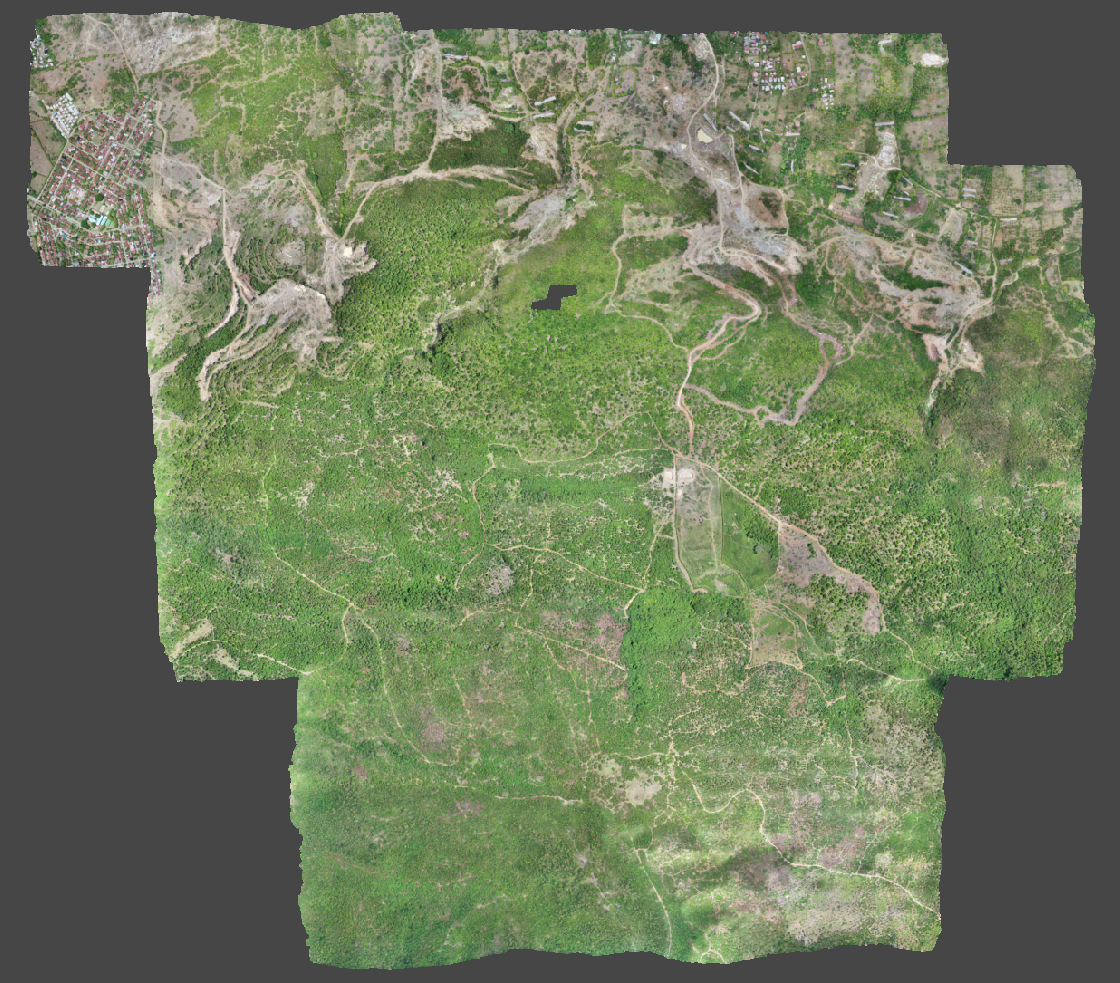
\includegraphics[width=1\linewidth]{image/Orthomosaic.png}
    \caption{Hasil output dari proses build Orthomosaic}
    \label{orthomosaic}
\end{figure}

\par Berdasarkan serangkaian proses mosaik yang telah dilaksanakan, kita memperoleh beberapa hasil, salah satunya adalah gambar orthomosaic. Dalam pelaksanaan proses mosaik menggunakan perangkat lunak Agisoft Metashape, terdapat beberapa kendala di mana pengaturan kualitas tertinggi tidak dapat diimplementasikan secara optimal. Berikut ini, penulis akan memaparkan secara rinci mengenai proses, konfigurasi kualitas, serta durasi yang diperlukan untuk menjalankan setiap tahapan. Informasi tersebut dapat dilihat secara komprehensif pada Tabel \ref{tabel hasil agisoft}.

\begin{table}[H]
\centering
\caption{Ringkasan detail Proses Mosaik menggunakan Agisoft Metashape}
\begin{tabular}{|c|c|c|c|c|}
\hline
\textbf{Proses} & \textbf{Pengaturan} & \textbf{Waktu} & \textbf{Penggunaan} & \textbf{Ukuran} \\
 & \textbf{Kualitas} & \textbf{proses} & \textbf{RAM} & \\
\hline
Align Photo & High & 1 jam 12 menit & 3,07 GB & 345,23 MB \\
\hline
Point Cloud & High & 13 jam 48 menit & 10,99 GB & 23,49 GB \\
\hline
Build Model & Medium & 3 jam 17 menit & 18,35 GB & 5,42 GB \\
\hline
Build Texture & - & 5 jam 52 menit & 14,27 GB & 5,42 GB \\
\hline
Build DEM & Ultra High & 9 menit & 476,43 MB & 4,37 GB \\
\hline
Build Orthomosaic & - & 2 jam 48 menit & 7,33 GB & 112,25 GB \\
\hline
\end{tabular}
\label{tabel hasil agisoft}
\end{table}

\par Data pada Tabel \ref{tabel hasil agisoft} menunjukkan kualitas tertinggi yang dapat diproses oleh spesifikasi komputer penulis. Upaya untuk menjalankan proses dengan kualitas yang lebih tinggi mengakibatkan perangkat lunak mengeluarkan pesan kesalahan "bad allocation". Berdasarkan diskusi dalam komunitas pengguna Agisoft Metashape, hal ini mengindikasikan bahwa komputer yang digunakan tidak memiliki kapasitas RAM yang memadai untuk memproses data sebanyak dan sebesar yang diinputkan. Kesalahan ini dapat terjadi ketika perangkat lunak tidak mampu mengalokasikan jumlah memori yang diperlukan untuk menyelesaikan tugas. Perlu dicatat bahwa hal ini tidak selalu berarti total RAM yang terpasang pada sistem tidak cukup, melainkan lebih kepada jumlah RAM yang tersedia saat operasi tersebut dilakukan. Untuk data dalam tabel yang ditandai dengan simbol (-), hal ini menunjukkan tidak adanya pilihan pengaturan kualitas sebelum proses berjalan dan cenderung menggunakan data olahan sebelumnya. Berdasarkan analisis tabel tersebut, dapat disimpulkan bahwa untuk menjalankan proses mosaik menggunakan Agisoft Metashape dengan data foto udara pada penelitian ini membutuhkan waktu total selama 27 jam 8 menit. Selain itu, dari kolom ukuran dapat diestimasi bahwa untuk menjalankan proyek ini dibutuhkan ruang penyimpanan kosong lebih dari 145,88 GB pada komputer. Informasi ini sangat penting untuk memastikan kesiapan sumber daya komputasi sebelum memulai proyek pengolahan data foto udara yang kompleks.

Selain mempertimbangkan pengaturan kualitas dan waktu pemrosesan yang dibutuhkan, keakuratan geometri merupakan aspek yang sangat penting untuk diperhatikan. Keakuratan ini tidak hanya mempengaruhi kualitas hasil akhir, tetapi juga berimplikasi pada validitas analisis spasial yang akan dilakukan selanjutnya. Untuk mengevaluasi tingkat keakuratan geometri ini, metode yang umum digunakan adalah pengukuran Root Mean Square Error (RMSE) pada Ground Control Points (GCP). Berikut pada Tabel \ref{tab:gcp_error} hasil analisis keakuratan geometri GCP menggunakan metode RMSE, yang memberikan gambaran kuantitatif tentang presisi spasial hasil mosaik.



\begin{table}[h]
\centering
\renewcommand{\arraystretch}{1.2}
\caption{Nilai RMSE dari control point Agisoft Metashape}
\begin{tabular}{|l|r|r|r|r|r|}
\hline
\textbf{Label} & \textbf{X error (cm)} & \textbf{Y error (cm)} & \textbf{Z error (cm)} & \textbf{Total (cm)} \\
\hline
GCP 1 & 12.2078 & 9.01173 & -0.423907 & 15.1796 \\
\hline
GCP 2 & 2.7889 & -2.22872 & 0.729977 & 3.65704 \\
\hline
GCP 3 & -8.37887 & -14.0609 & -16.0817 & 22.9463 \\
\hline
GCP 5 & -6.22628 & -2.69796 & 7.9977 & 10.4885 \\
\hline
GCP 6 & 1.36338 & -1.11841 & 10.526 & 10.6727 \\
\hline
GCP 7 & -9.55819 & 6.92873 & -11.9352 & 16.7874 \\
\hline
GCP 9 & -1.95363 & 10.282 & -0.424963 & 10.4745 \\
\hline
GCP 10 & -2.69963 & -11.9162 & 16.2295 & 20.3145 \\
\hline
GCP 11 & 2.29594 & 3.137 & 0.0377947 & 3.88761 \\
\hline
GCP 13 & -7.8657 & -1.03983 & -9.05366 & 12.0382 \\
\hline
GCP 14 & 7.97648 & 6.55242 & 9.0998 & 13.761 \\
\hline
GCP 15 & 6.74509 & 6.35585 & 8.45827 & 11.5958 \\
\hline
GCP 18 & -1.21502 & -2.07861 & -5.9071 & 6.37893 \\
\hline
GCP 19 & 6.45574 & -1.36734 & 1.20425 & 6.70794 \\
\hline
GCP 23 & -5.15025 & -6.04869 & -9.21289 & 12.1651 \\
\hline
GCP 24 & 5.17219 & 0.351325 & -1.58555 & 5.42116 \\
\hline
\textbf{Total} & \textbf{6.22405} & \textbf{6.73281} & \textbf{8.66123} & \textbf{12.6129} \\
\hline
\end{tabular}
\label{tab:gcp_error}
\end{table}

Berdasarkan hasil analisis pada Tabel \ref{tab:gcp_error}, diperoleh gambaran komprehensif mengenai akurasi pengukuran. Total RMSE mencapai 12,6129 cm, mencerminkan kesalahan gabungan dari semua arah. Kesalahan pada sumbu X (timur-barat) sebesar 6,22408 cm, sementara pada sumbu Y (utara-selatan) sedikit lebih tinggi yaitu 6,73281 cm. Kesalahan vertikal atau Z error menunjukkan nilai tertinggi sebesar 8,66123 cm, mengindikasikan bahwa pengukuran ketinggian cenderung kurang presisi dibandingkan pengukuran horizontal. Dari data tersebut, dapat dihitung RMSEr (Root Mean Square Error radial) yang merepresentasikan kesalahan radial horizontal gabungan, yaitu sebesar 9,17 cm. Nilai ini diperoleh dari akar kuadrat jumlah kuadrat RMSE X dan Y. Secara keseluruhan, hasil ini menunjukkan bahwa pengukuran memiliki tingkat akurasi yang cukup baik dengan kisaran kesalahan antara 10-13 cm, namun masih terdapat ruang untuk peningkatan, terutama dalam aspek pengukuran vertikal yang menunjukkan variasi lebih besar dibandingkan pengukuran horizontal.

Setelah memperoleh data RMSE dari proses mosaik, langkah berikutnya adalah menghitung nilai Circular Error (CE90) dan Linear Error (LE90). Perhitungan ini mengacu pada rumus yang diatur oleh Badan Informasi Geospasial tahun 2014. Hasil perhitungan ini dapat dilihat pada Tabel \ref{tab:hasil_perhitungan ce}, yang memberikan gambaran tentang seberapa akurat data geospasial tersebut setelah proses mosaik.

\begin{table}[H]
\centering
\caption{Hasil Perhitungan RMSEr, RMSEz, CE90, dan LE90 pada perangkat lunak Agisoft Metashape}
\begin{tabular}{|l|c|}
\hline
\textbf{Komponen} & \textbf{Nilai (cm)} \\
\hline
RMSEr & 9,17 \\
RMSEz & 8,66 \\
CE90 & 13,92 \\
LE90 & 14,29 \\
\hline
\end{tabular}
\label{tab:hasil_perhitungan ce}
\end{table}

\subsection{PIX4Dmapper}

\par Dalam PIX4Dmapper, proses mosaik melibatkan beberapa tahap utama pemrosesan. Langkah pertama adalah mengimpor seluruh foto udara ke dalam perangkat lunak PIX4Dmapper. Penting untuk memastikan bahwa semua foto udara telah dimasukkan dengan lengkap, tanpa ada satu pun yang tertinggal. Initial Processing merupakan tahap awal yang krusial dalam proses menghasilkan orthomosaik dari foto udara yang diambil menggunakan drone. Pada tahap ini, PIX4Dmapper akan melakukan kalibrasi kamera, mencari titik yang sama antar gambar (keypoints). Perangkat lunak juga menggunakan data GPS dari drone untuk memposisikan foto-foto dan mengidentifikasi sudut pengambilan gambar drone terhadap permukaan lahan yang dipotret. Hasil dari proses ini berupa titik-titik informasi relatif dari setiap foto dalam ruang tiga dimensi seperti pada Gambar \ref{hasil_initialprocessing} berikut.

\begin{figure} [H]
    \centering
    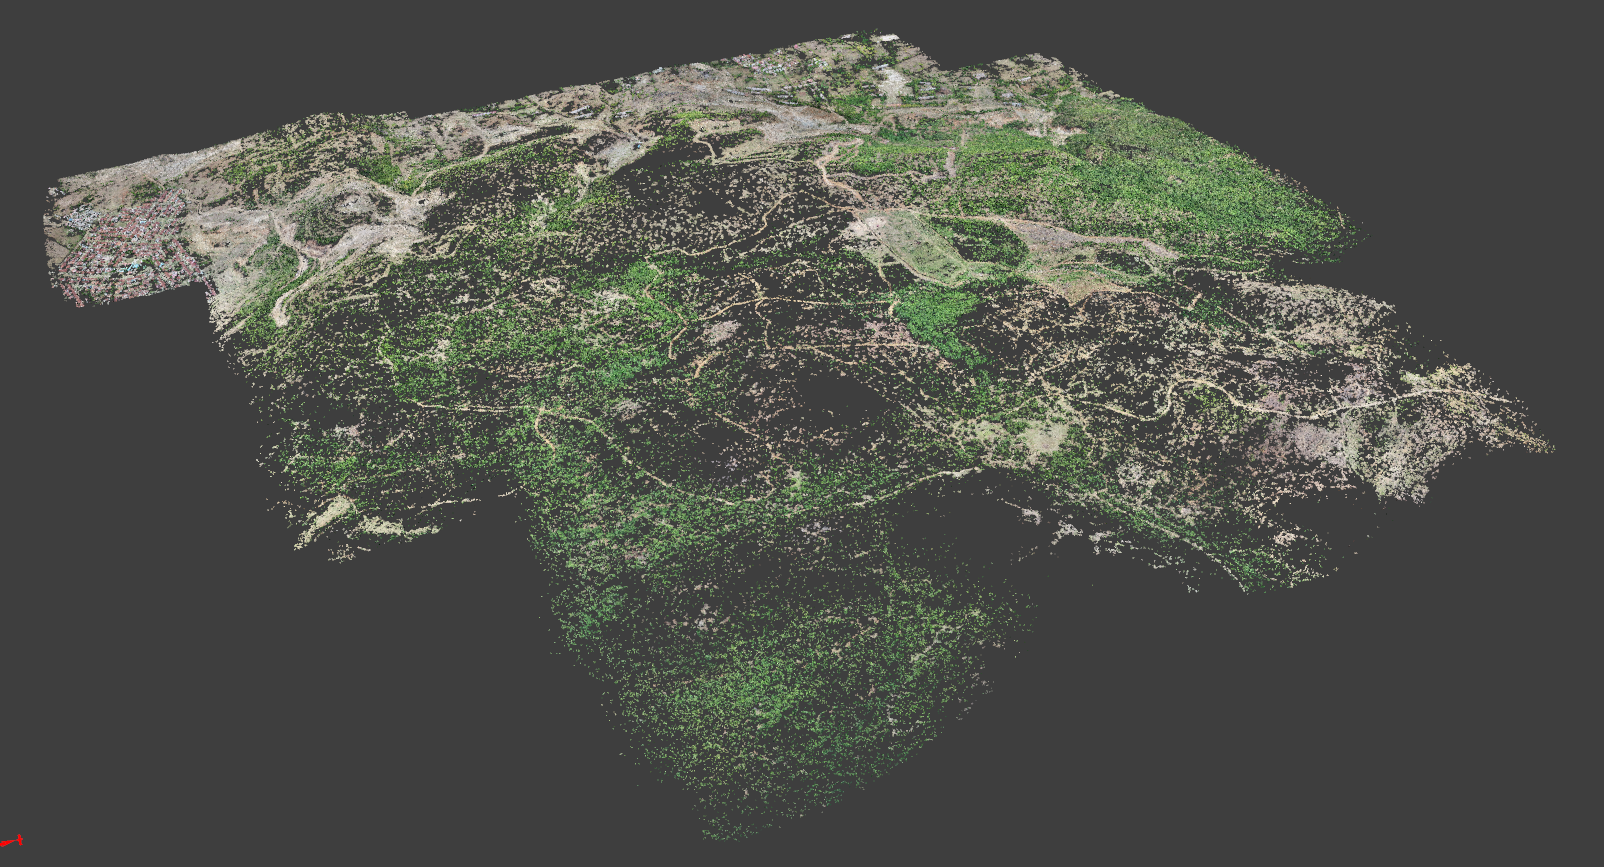
\includegraphics[width=1\linewidth]{image/initial processing.png}
    \caption{Hasil output dari proses initial processing}
    \label{hasil_initialprocessing}
\end{figure}

hasil ini akan menjadi dasar untuk tahap-tahap selanjutnya dalam pembuatan orthomosaik. Setelah Initial Processing selesai, pengguna dapat memeriksa hasil dan melakukan penyesuaian jika diperlukan sebelum melanjutkan ke tahap berikutnya seperti Point Cloud and Mesh, DSM, Orthomosaic and Index, dan sebagainya. Dalam penelitian ini, setelah melakukan initial processing, langkah selanjutnya yang krusial adalah penyesuaian dan penginputan Ground Control Point (GCP). Proses ini sangat penting untuk meningkatkan akurasi geometri dari model yang dihasilkan. GCP adalah titik-titik referensi di lapangan dengan koordinat yang diketahui secara akurat, yang digunakan untuk mengkalibrasi dan mengoreksi data pemetaan udara. Dengan memasukkan koordinat GCP yang tepat ke dalam software, kita dapat mengurangi kesalahan posisi dan meningkatkan ketelitian pemetaan secara keseluruhan. Hal ini memastikan bahwa hasil akhir pemetaan memiliki akurasi spasial yang tinggi dan dapat diandalkan untuk berbagai aplikasi. GCP yang digunakan juga sama seperti yang digunakan pada proses menggunakan Agisoft Metashape dan berjumlah 16 GCP. Distribusi spasial dari titik-titik GCP dapat dilihat pada Gambar \ref{penyebaran  pix}. Sementara itu, tahapan penyesuaian koordinat GCP terhadap citra drone diilustrasikan pada Gambar dan \ref{gcpakurat pix}, memberikan gambaran visual tentang proses penyelarasan yang dilakukan. 

\begin{figure} [H]
    \centering
    \frame{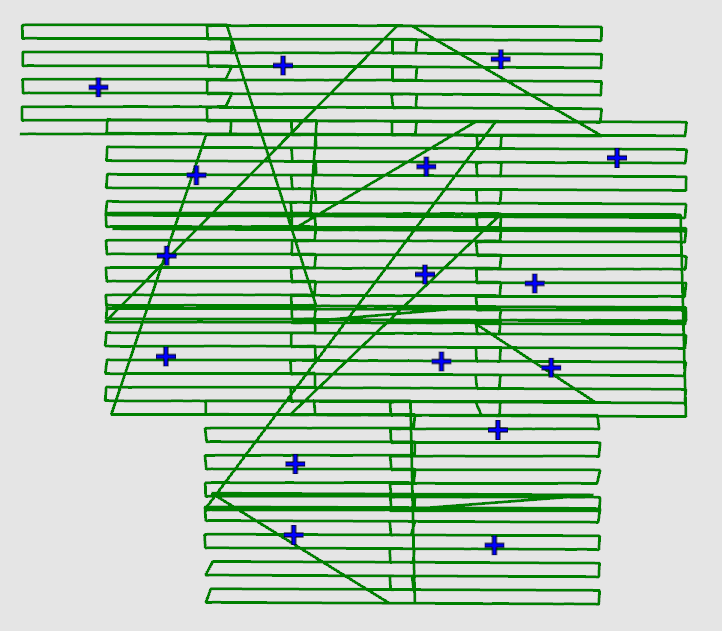
\includegraphics[width = 13cm]{image/penyebaran GCP.png}}
    \caption{Penyebaran titik Ground Control Point ditandai simbol (+).}
    \label{penyebaran pix}
\end{figure}

\begin{figure} [H]
    \centering
    \frame{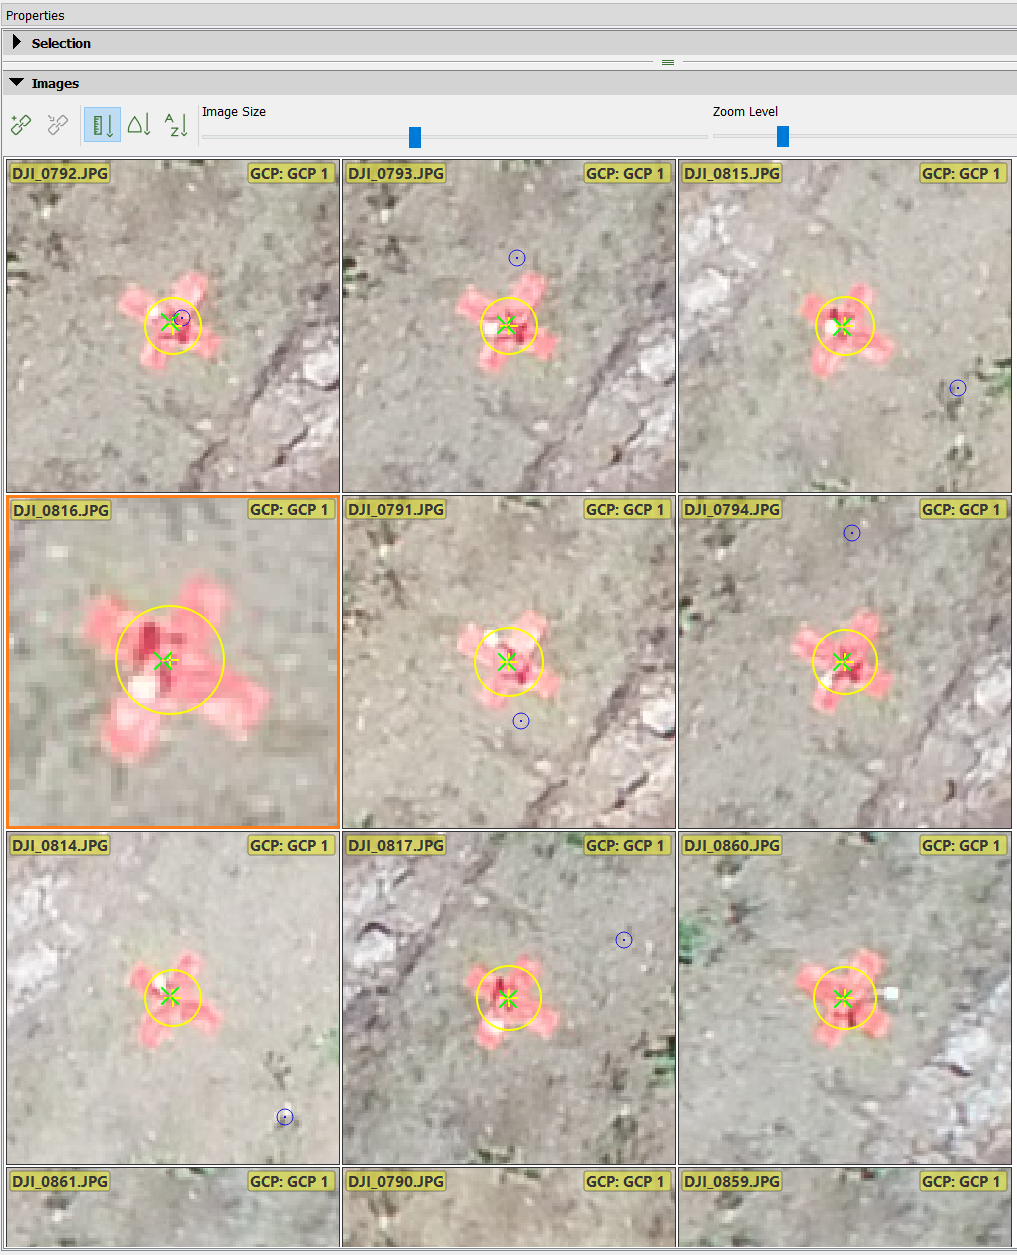
\includegraphics[width = 11.5cm]{image/penentuan GCP.png}}
    \caption{Proses penyesuaian Ground Control Point.}
    \label{gcpakurat pix}
\end{figure}

Tahap selanjutnya adalah Point Cloud and Mesh, sebuah proses terintegrasi dalam PIX4Dmapper yang memerlukan waktu lebih lama dan sumber daya perangkat keras yang intensif. Dalam tahap ini, perangkat lunak tidak hanya menghasilkan titik-titik 3D (point cloud) yang secara akurat merepresentasikan permukaan objek atau area lahan yang dipetakan, tetapi juga langsung menghasilkan mesh 3D. PIX4Dmapper memanfaatkan informasi dari foto-foto yang telah diproses sebelumnya untuk menentukan posisi 3D dari fitur-fitur yang terlihat pada setiap gambar dengan presisi tinggi. Hasil dari proses ini adalah kumpulan titik-titik padat yang mewakili struktur permukaan, serta mesh yang menghubungkan titik-titik tersebut menjadi model 3D yang solid. Tingkat kepadatan point cloud yang dihasilkan jauh lebih tinggi dibandingkan tie points pada tahap initial processing. Dalam penelitian ini, proses Point Cloud and Mesh memakan waktu sekitar 5 jam 37 menit dengan pengaturan kualitas Low (Fast), menghasilkan lebih dari 131 juta titik dan mesh yang sesuai. Penggabungan proses point cloud dan mesh ini memungkinkan PIX4Dmapper untuk menghasilkan model 3D yang lebih efisien dan siap digunakan. Visualisasi hasil dari tahap Point Cloud and Mesh dapat dilihat pada Gambar \ref{point cloud pix}, \ref{mesh pix}. Proses terintegrasi ini merupakan langkah penting dalam menghasilkan model 3D yang detail dan akurat untuk analisis lebih lanjut.

\begin{figure} [H]
    \centering
    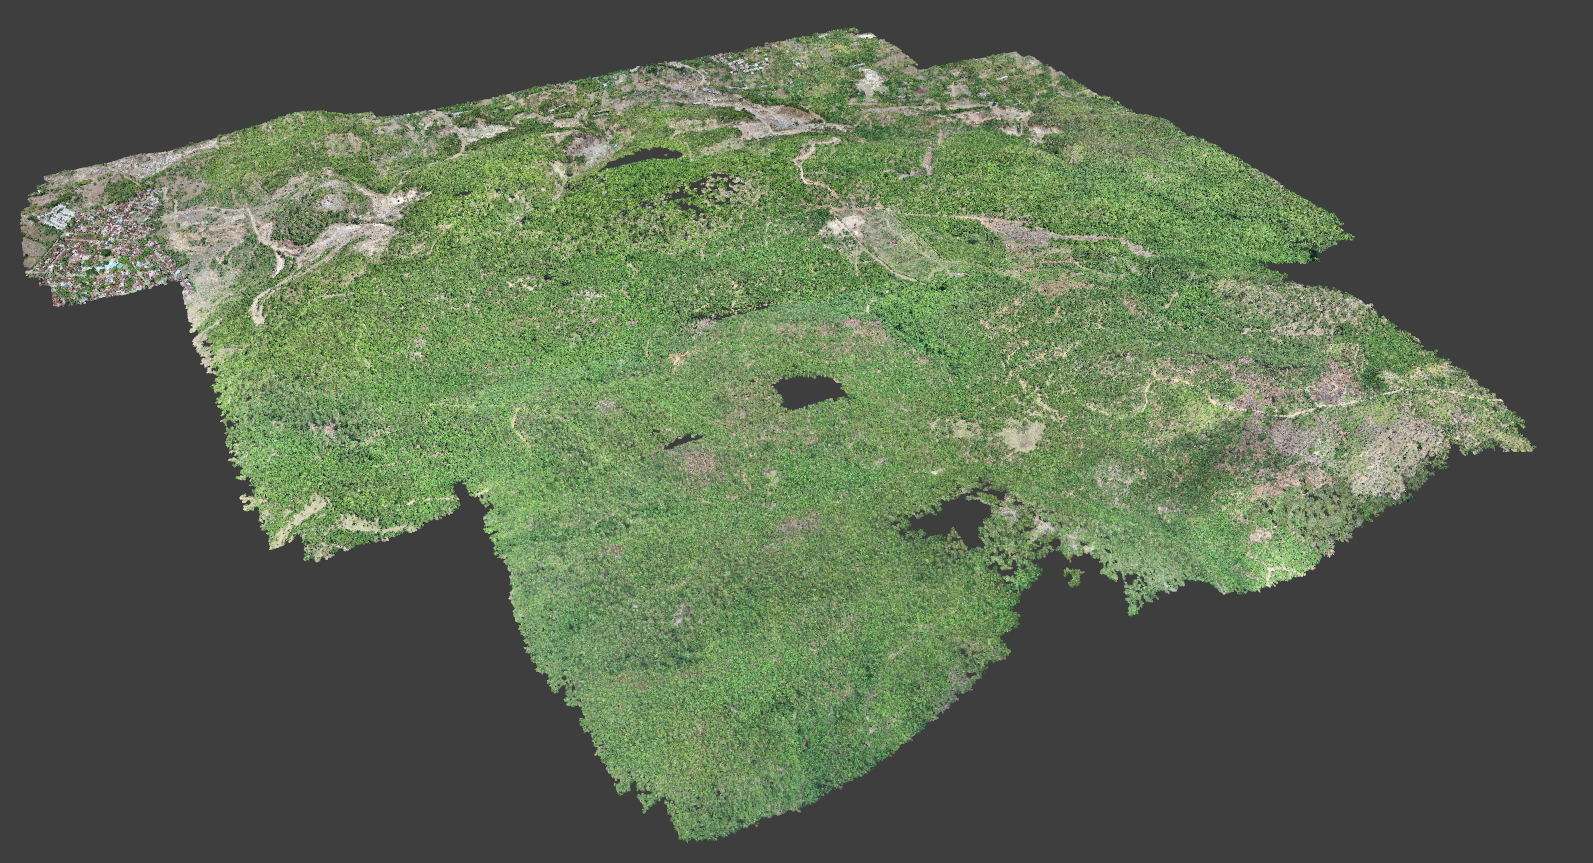
\includegraphics[width=1\linewidth]{image/point cloud.png}
    \caption{Hasil output dari proses point cloud}
    \label{point cloud pix}
\end{figure}

\begin{figure} [H]
    \centering
    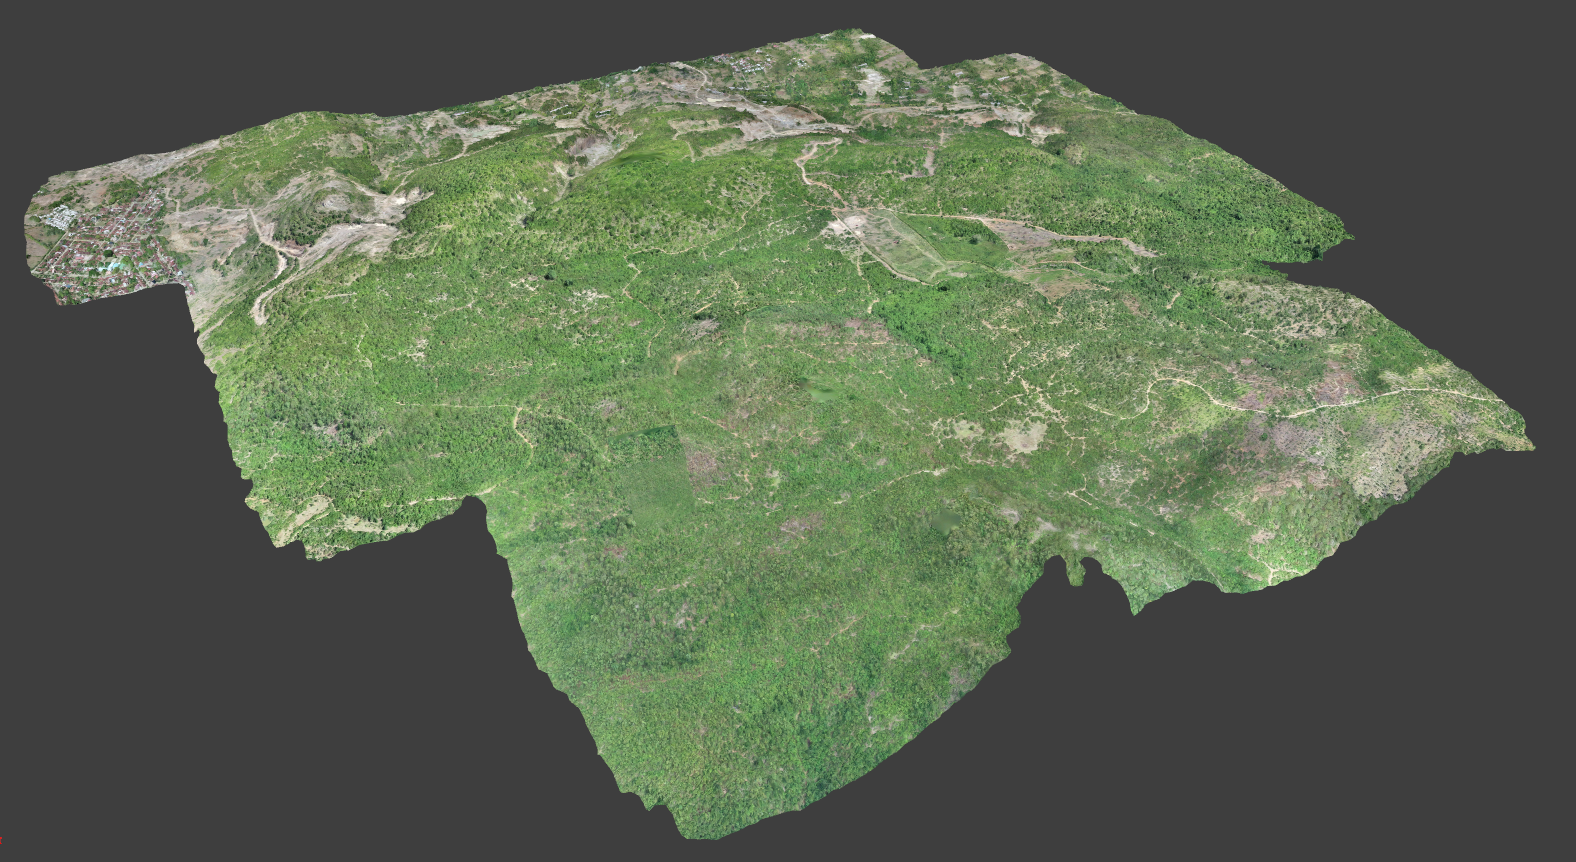
\includegraphics[width=1\linewidth]{image/mesh.png}
    \caption{Hasil output dari proses mesh}
    \label{mesh pix}
\end{figure}

Setelah proses pembuatan point cloud dan mesh selesai, perangkat lunak PIX4Dmapper akan melanjutkan ke tahap selanjutnya, yaitu pembuatan DSM (Digital Surface Model), dan orthomosaic.
Proses DSM menghasilkan model elevasi digital yang menggambarkan permukaan bumi termasuk semua objek di atasnya seperti bangunan dan vegetasi. DSM dibuat dengan menggunakan data ketinggian dari point cloud yang telah dihasilkan sebelumnya. Orthomosaic adalah citra foto udara yang telah dikoreksi secara geometris sehingga skala yang dihasilkan seragam dan dapat digunakan untuk pengukuran jarak dan luas yang akurat. Proses ini menggabungkan dan menyesuaikan berbagai foto udara menjadi satu citra yang detail dan tergeoreferensi. Hasil output dari proses DSM dan orthomosaic dapat dilihat pada Gambar \ref{dsm ortho}. DSM biasanya ditampilkan sebagai peta kontur atau visualisasi 3D berwarna, sementara orthomosaic akan terlihat seperti foto udara yang sangat detail dan akurat secara geometris dari area yang dipetakan.

\begin{figure} [H]
    \centering
    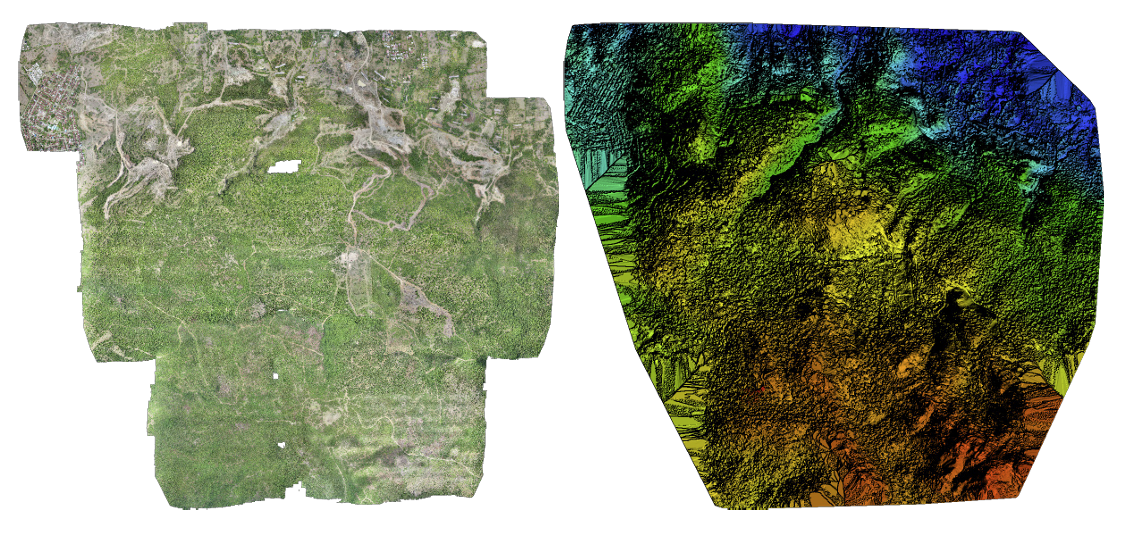
\includegraphics[width=1\linewidth]{image/DSM dan ortho.png}
    \caption{Hasil output DSM dan Orthomosaic}
    \label{dsm ortho}
\end{figure}

Hasil output orthomosaic dari perangkat lunak PIX4Dmapper mencapai resolusi yang sangat tinggi, yaitu 4,4 cm/pixel. Resolusi ini menunjukkan tingkat detail yang luar biasa dalam pemetaan menggunakan teknologi fotogrametri udara. Setiap pixel dalam citra orthomosaic mewakili area seluas 4,4 cm x 4,4 cm di permukaan bumi, memungkinkan identifikasi dan analisis objek-objek kecil dengan sangat jelas, seperti vegetasi individual, fitur-fitur arsitektur pada bangunan, infrastruktur jalan yang detail, dan objek-objek kecil di permukaan tanah. Pencapaian resolusi setinggi ini merupakan hasil dari kombinasi kualitas kamera drone yang digunakan, ketinggian terbang yang relatif rendah, tingkat overlap foto yang tinggi, serta kemampuan pengolahan canggih dari PIX4Dmapper. 

Berdasarkan serangkaian proses mosaik yang telah dilaksanakan menggunakan PIX4Dmapper, kita memperoleh beberapa hasil, salah satunya adalah orthomosaic. Dalam pelaksanaan proses mosaik menggunakan perangkat lunak PIX4Dmapper, terdapat beberapa pertimbangan dalam pemilihan pengaturan kualitas untuk mengoptimalkan hasil dan efisiensi waktu pemrosesan. Berikut ini, penulis akan memaparkan secara rinci mengenai proses, konfigurasi kualitas, serta durasi yang diperlukan untuk menjalankan setiap tahapan dalam PIX4Dmapper. Informasi tersebut dapat dilihat secara komprehensif pada Tabel \ref{runningpix}.

\begin{table}[h]
\centering
\caption{Ringkasan detail proses mosaik menggunakan PIX4Dmapper}
\begin{tabular}{|c|c|c|}
\hline
\textbf{Proses} & \textbf{Pengaturan kualitas} & \textbf{Waktu proses}\\
\hline
Initial Processing & Full & 4 jam 10 menit \\
\hline
Point Cloud & Low & 4 jam 46 menit \\
\hline
Build mesh & Medium & 51 menit \\
\hline
Build DSM & Sharp & 1 jam 22 menit \\
\hline
Build Orthomosaic & - & 5 jam 50 menit \\
\hline
\end{tabular}
\label{runningpix}
\end{table}

Data pada Tabel \ref{runningpix} menunjukkan kualitas tertinggi yang dapat diproses oleh spesifikasi komputer penulis menggunakan PIX4Dmapper. Upaya untuk menjalankan proses dengan kualitas yang lebih tinggi dapat mengakibatkan perangkat lunak mengeluarkan pesan kesalahan terkait memori tidak mencukupi ataupun perangkat lunak akan mengalami force close. Kesalahan ini dapat terjadi ketika perangkat lunak tidak mampu mengalokasikan jumlah memori yang diperlukan untuk menyelesaikan tugas.Perlu dicatat bahwa hal ini tidak selalu berarti total RAM yang terpasang pada sistem tidak cukup, melainkan lebih kepada jumlah RAM yang tersedia saat operasi tersebut dilakukan. Untuk data dalam tabel yang ditandai dengan simbol (-), hal ini menunjukkan penggunaan pengaturan default PIX4Dmapper atau penggunaan data olahan dari tahap sebelumnya tanpa opsi pengaturan tambahan. Berdasarkan analisis tabel tersebut, dapat disimpulkan bahwa untuk menjalankan proses mosaik menggunakan PIX4Dmapper dengan data foto udara pada penelitian ini membutuhkan waktu total selama 16 jam 59 menit. Waktu pemrosesan ini mencakup semua tahapan dari importasi gambar hingga generasi orthomosaic akhir. Sayangnya, pada hasil report dari aplikasi PIX4Dmapper tidak menyertakan informasi detail mengenai penggunaan RAM dan penyimpanan pada setiap prosesnya.

\begin{table}[H]
\centering
\renewcommand{\arraystretch}{1}
\caption{Nilai RMSE dari control point PIX4Dmapper}
\begin{tabular}{|l|r|r|r|r|r|}
\hline
\textbf{Label} &\textbf{ X error (cm)} &\textbf{ Y error (cm)} & \textbf{Z error (cm)} & \textbf{Total (cm)} \\
\hline
GCP 1 (3D) & -0.9 & -1.5 & -0.2 & 1.75 \\
\hline
GCP 2 (3D) & -0.5 & -1.0 & 0.3 & 1.15 \\
\hline
GCP 3 (3D) & -2.2 & 1.8 & 0.2 & 2.85 \\
\hline
GCP 5 (3D) & 5.6 & 7.6 & -1.6 & 9.65 \\
\hline
GCP 6 (3D) & -1.2 & 0.5 & -1.3 & 1.85 \\
\hline
GCP 7 (3D) & -1.4 & -3.2 & 0.2 & 3.50 \\
\hline
GCP 9 (3D) & -2.8 & -5.9 & 1.0 & 6.60 \\
\hline
GCP 10 (3D) & 5.6 & 10.3 & -0.9 & 11.75 \\
\hline
GCP 11 (3D) & -2.4 & -0.8 & 5.8 & 6.35 \\
\hline
GCP 13 (3D) & -0.1 & 12.7 & 2.3 & 12.90 \\
\hline
GCP 14 (3D) & -3.6 & -8.7 & -0.9 & 9.45 \\
\hline
GCP 15 (3D) & 2.8 & -1.7 & -2.5 & 4.10 \\
\hline
GCP 18 (3D) & 94.1 & -132.1 & -85.0 & 183.45 \\
\hline
GCP 19 (3D) & -0.8 & -0.3 & 2.9 & 3.05 \\
\hline
GCP 23 (3D) & 227.2 & -30.4 & -5.5 & 229.85 \\
\hline
GCP 24 (3D) & 1.8 & 1.9 & -0.3 & 2.60 \\
\hline
\textbf{RMS Error} & \textbf{61.5358} & \textbf{34.2995} & \textbf{21.3708} & \textbf{73.31} \\
\hline
\end{tabular}
\label{tab:gcp_error_cm}
\end{table}

Selain pengaturan kualitas dan efisiensi waktu, pada Tabel \ref{tab:gcp_error_cm} dapat dilihat hasil selanjutnya yang akan dipaparkan berkaitan dengan keakuratan geometri menggunakan Ground Control Points (GCP) dengan metode Root Mean Square Error (RMSE), yang memberikan gambaran kuantitatif mengenai presisi hasil mosaik. Analisis ini sangat penting untuk menilai kualitas dan keandalan peta yang dihasilkan. Dengan menggunakan titik-titik kontrol di lapangan (GCP) dan menghitung tingkat kesalahan (RMSE), dapat diketahui seberapa tepat gambar mosaik yang dihasilkan. Hal ini membantu dalam menentukan apakah hasil pemetaan sudah memenuhi standar untuk berbagai keperluan yang berbeda.

Berdasarkan hasil analisis pada Tabel 4.8, diperoleh gambaran komprehensif mengenai akurasi pengukuran. Total RMSE mencapai 73,31 cm, mencerminkan kesalahan gabungan dari semua arah. Kesalahan pada sumbu X (timur-barat) sebesar 61,5358 cm, sementara pada sumbu Y (utara-selatan) lebih rendah yaitu 34,2995 cm. Kesalahan vertikal atau Z error menunjukkan nilai terendah sebesar 21,3708 cm, mengindikasikan bahwa pengukuran ketinggian cenderung lebih presisi dibandingkan pengukuran horizontal. Dari data tersebut, dapat dihitung RMSEr (Root Mean Square Error radial) yang merepresentasikan kesalahan radial horizontal gabungan, yaitu sebesar 70,42 cm. Nilai ini diperoleh dari akar kuadrat jumlah kuadrat RMSE X dan Y. Secara keseluruhan, hasil ini menunjukkan bahwa pengukuran memiliki tingkat akurasi yang bervariasi dengan kisaran kesalahan yang cukup besar, terutama pada pengukuran horizontal. Terlihat adanya beberapa titik kontrol dengan error yang sangat tinggi, seperti GCP 23 (3D) dengan total error mencapai 229,85 cm, yang secara signifikan mempengaruhi nilai RMSE keseluruhan. Pengukuran vertikal menunjukkan konsistensi yang lebih baik dibandingkan pengukuran horizontal, namun masih terdapat ruang untuk peningkatan akurasi secara keseluruhan, terutama dalam mengurangi variasi error yang ekstrem pada beberapa titik kontrol.

Setelah memperoleh data RMSE dari proses mosaik, langkah berikutnya adalah menghitung nilai Circular Error (CE90) dan Linear Error (LE90). Perhitungan ini mengacu pada rumus yang diatur oleh Badan Informasi Geospasial tahun 2014. Hasil perhitungan ini dapat dilihat pada Tabel \ref{tab:hasil_perhitungan le}, yang memberikan gambaran tentang seberapa akurat data geospasial tersebut setelah proses mosaik.

\begin{table}[H]
\centering
\caption{Hasil Perhitungan RMSEr, RMSEz, CE90, dan LE90 pada perangkat lunak PIX4Dmapper}
\begin{tabular}{|l|c|}
\hline
\textbf{Komponen} & \textbf{Nilai (cm)} \\
\hline
RMSEr & 70.45 \\
RMSEz & 21,37 \\
CE90 & 106,91 \\
LE90 & 35,26 \\
\hline
\end{tabular}
\label{tab:hasil_perhitungan le}
\end{table}

\section{Analisis Perbandingan}

\par Setelah menyelesaikan proses mosaik menggunakan dua perangkat lunak berbeda, yakni Agisoft Metashape dan PIX4Dmapper, dengan dataset identik berupa 4.701 foto udara dan 16 titik koordinat GCP (Ground Control Points), langkah berikutnya adalah melakukan analisis komparatif terhadap hasil mosaik. Perbandingan ini akan berfokus pada beberapa aspek kunci, meliputi keakuratan geometri, resolusi spasial, efisiensi waktu pemrosesan, serta kualitas visual secara detail pada beberapa titik sampel orthomosaik. Analisis mendalam ini bertujuan untuk mengevaluasi kinerja kedua perangkat lunak dalam menghasilkan orthomosaik yang presisi dan berkualitas tinggi, sehingga dapat memberikan wawasan komprehensif mengenai keunggulan dan kelemahan masing-masing perangkat lunak dalam konteks pengolahan data foto udara.

\subsection{Akurasi Geometri}

Berdasarkan Tabel \ref{tab:perbandingan} yang menunjukkan perbandingan hasil perhitungan RMSEr, RMSEz, CE90, dan LE90 pada perangkat lunak Agisoft PIX4Dmapper dan Agisoft Metashape dalam satuan sentimeter (cm), dapat disimpulkan:
PIX4Dmapper masih menghasilkan nilai kesalahan yang lebih tinggi dibandingkan Agisoft Metashape untuk semua parameter. RMSEr PIX4Dmapper (70,45 cm) lebih besar daripada Metashape (9,17 cm). Pola yang sama terlihat untuk RMSEz, CE90, dan LE90.

\begin{table}[H]
\centering
\begin{tabular}{|l|c|c|}
\hline
\textbf{Komponen} & \textbf{Agisoft Metashape (cm)} & \textbf{PIX4Dmapper (cm)} \\
\hline
RMSEr  & 9,17 & 70,45 \\
RMSEz  & 8,66 & 21,37 \\
CE90  & 13,92 & 106,91 \\
LE90  & 14,29 & 35,26 \\
\hline
\end{tabular}
\caption{Perbandingan Hasil Perhitungan RMSEr, RMSEz, CE90, dan LE90 pada Perangkat Lunak Agisoft PIX4Dmapper dan Agisoft Metashape}
\label{tab:perbandingan}
\end{table}

Berdasarkan perbandingan nilai CE90 dan LE90 yang dihasilkan oleh Agisoft Metashape dan PIX4Dmapper dengan standar ketelitian peta RBI, dapat disimpulkan bahwa kedua perangkat lunak mampu menghasilkan mosaik dengan ketelitian tinggi. Agisoft Metashape menunjukkan performa yang sangat baik dengan nilai CE90 13,92 cm dan LE90 14,29 cm, sementara PIX4Dmapper menghasilkan nilai CE90 106,91 cm dan LE90 35,26 cm. Ketika dibandingkan dengan Tabel 2.2 Ketelitian Peta RBI, kedua hasil ini menunjukkan potensi untuk memenuhi standar ketelitian pada skala peta yang berbeda.

\begin{itemize}
    \item \textbf{Agisoft Metashape:} Mampu mencapai ketelitian peta RBI untuk skala 1:1.000 kelas 1. Nilai CE90 dan LE90 yang dihasilkan bahkan lebih baik dari batas maksimum yang ditetapkan untuk skala ini (0,2 m untuk keduanya), menunjukkan potensi untuk ketelitian pada skala yang lebih besar jika standar tersedia.
    \item \textbf{PIX4Dmapper:} Dapat mencapai ketelitian peta RBI untuk skala 1:2.500 kelas 1. Hasil ini memenuhi dengan baik standar yang ditetapkan untuk skala tersebut, di mana batas maksimum CE90 dan LE90 adalah 0,5 m.
\end{itemize}

Ketelitian peta RBI tertinggi yang dapat dicapai berdasarkan hasil mosaik adalah skala 1:1.000 kelas 1 untuk Agisoft Metashape, dengan potensi untuk skala yang lebih besar, dan skala 1:2.500 kelas 1 untuk PIX4Dmapper. Kedua perangkat lunak menghasilkan mosaik yang memenuhi standar ketelitian tinggi untuk pemetaan RBI, dengan Agisoft Metashape menunjukkan keunggulan dalam mencapai ketelitian untuk skala peta yang lebih besar.

\subsection{Resolusi}

hasil orthomosaik dari kedua perangkat lunak menunjukkan resolusi yang sangat tinggi, dengan PIX4Dmapper menghasilkan resolusi yang sedikit lebih tinggi dibandingkan Agisoft Metashape. Orthomosaik yang dihasilkan oleh PIX4Dmapper memiliki resolusi 77405x69710 piksel, sementara Agisoft Metashape menghasilkan resolusi 75364x67824 piksel. Perbedaan ini menunjukkan bahwa PIX4Dmapper mampu menghasilkan citra dengan detail yang sedikit lebih tinggi, dengan selisih sekitar 2041 piksel pada dimensi panjang dan 1886 piksel pada dimensi lebar. Meskipun perbedaan ini ada, kedua hasil dapat dianggap memiliki kualitas resolusi yang sangat baik untuk keperluan pemetaan dan analisis spasial yang membutuhkan tingkat detail tinggi. Perbedaan resolusi ini mungkin tidak signifikan untuk sebagian besar aplikasi praktis, namun dapat menjadi pertimbangan dalam proyek-proyek yang memerlukan tingkat presisi yang sangat tinggi.

Begitu pula terkait ground resolution dari hasil pemrosesan Agisoft Metashape menunjukkan ground resolution sebesar 4,54 cm/pixel, sedangkan Pix4Dmapper menghasilkan 4,4 cm/pixel. Perbedaan ini menunjukkan bahwa secara umum, Pix4Dmapper berhasil menghasilkan detail yang sedikit lebih halus pada permukaan objek yang dipetakan dibandingkan dengan Agisoft Metashape. Namun, perbedaan sebesar 0,14 cm/pixel ini relatif kecil dan mungkin tidak terlalu signifikan secara visual, terutama jika dilihat pada skala yang lebih besar.

\subsection{Waktu Pemrosesan}

Setelah selesai melakukan proses mosaik pada kedua perangkat lunak, yaitu Agisoft Metashape dan PIX4Dmapper berdasarkan pengaturan kualitas masing-masing, maka diperoleh data waktu yang dibutuhkan untuk setiap tahap proses pada kedua aplikasi, seperti yang terlihat pada Tabel 4.11 berikut.

\begin{table}[h]
\centering
\caption{Perbandingan Proses, Waktu, dan Kualitas antara Agisoft Metashape dan PIX4Dmapper}
\begin{tabular}{|l|c|c|c|c|}
\hline
\multirow{2}{*}{Proses} & \multicolumn{2}{c|}{Agisoft Metashape} & \multicolumn{2}{c|}{PIX4Dmapper} \\
\cline{2-5}
 & Kualitas & Waktu & Kualitas & Waktu \\
\hline
Initial Processing & High & 1 jam 12 menit & Full & 4 jam 10 menit \\
\hline
Point Cloud & High & 13 jam 48 menit & Low & 4 jam 46 menit \\
\hline
Build Model / mesh & Medium & 3 jam 17 menit & Medium & 51 menit \\
\hline
Build Texture & - & 5 jam 52 menit & - & - \\
\hline
Build DEM / DSM & Ultra High & 9 menit & Sharp & 1 jam 22 menit \\
\hline
Build Orthomosaic & - & 2 jam 48 menit & - & 5 jam 50 menit \\
\hline
\end{tabular}
\label{tab:perbandinganwaktu}
\end{table}

Berdasarkan Tabel \ref{tab:perbandinganwaktu
}, dapat disimpulkan bahwa Agisoft Metashape dan PIX4Dmapper memiliki karakteristik pemrosesan yang berbeda. Meskipun pada pandangan pertama Agisoft Metashape tampak memerlukan waktu pemrosesan yang lebih panjang secara keseluruhan, penting untuk mempertimbangkan bahwa durasi pemrosesan sangat dipengaruhi oleh pengaturan kualitas yang dipilih sebelum proses dimulai. Analisis lebih mendalam menunjukkan bahwa dalam beberapa tahapan dengan pengaturan kualitas yang setara, Agisoft Metashape justru mengungguli PIX4Dmapper dalam hal efisiensi waktu. Sebagai contoh, pada tahap Initial Processing, Build DEM dan Orthomosaic, Agisoft Metashape menyelesaikan tugas jauh lebih cepat dibandingkan PIX4Dmapper. Di sisi lain, PIX4Dmapper menunjukkan keunggulan signifikan dalam proses pembangunan mesh, dengan waktu pemrosesan yang jauh lebih singkat dibandingkan Agisoft Metashape. Hal ini menggambarkan bahwa masing-masing software memiliki kekuatan tersendiri dalam aspek-aspek tertentu dari alur kerja fotogrametri.

\subsection{Kualitas Visual}

Analisis krusial dalam proses mosaik pada penelitian ini adalah perbandingan hasil visual dari kedua perangkat lunak. Tahap ini melibatkan pengambilan beberapa sampel gambar dari orthomosaik yang dihasilkan oleh kedua perangkat lunak di berbagai lokasi yang berbeda. Lokasi-lokasi yang dipilih mencakup komplek perumahan, jalan, lereng perbukitan, dan hutan dengan vegetasi lebat. Pemilihan lokasi yang beragam ini bertujuan untuk mengevaluasi kinerja perangkat lunak dalam menangani berbagai jenis terrain dan fitur permukaan. Hasil perbandingan visual ini disajikan secara komprehensif dalam Gambar 4.18, 4.19, 4.20, dan 4.21. Melalui analisis ini, dapat diperoleh pemahaman mendalam tentang kualitas dan akurasi orthomosaik yang dihasilkan oleh masing-masing perangkat lunak dalam berbagai kondisi lapangan.

\begin{figure} [H]
    \centering
    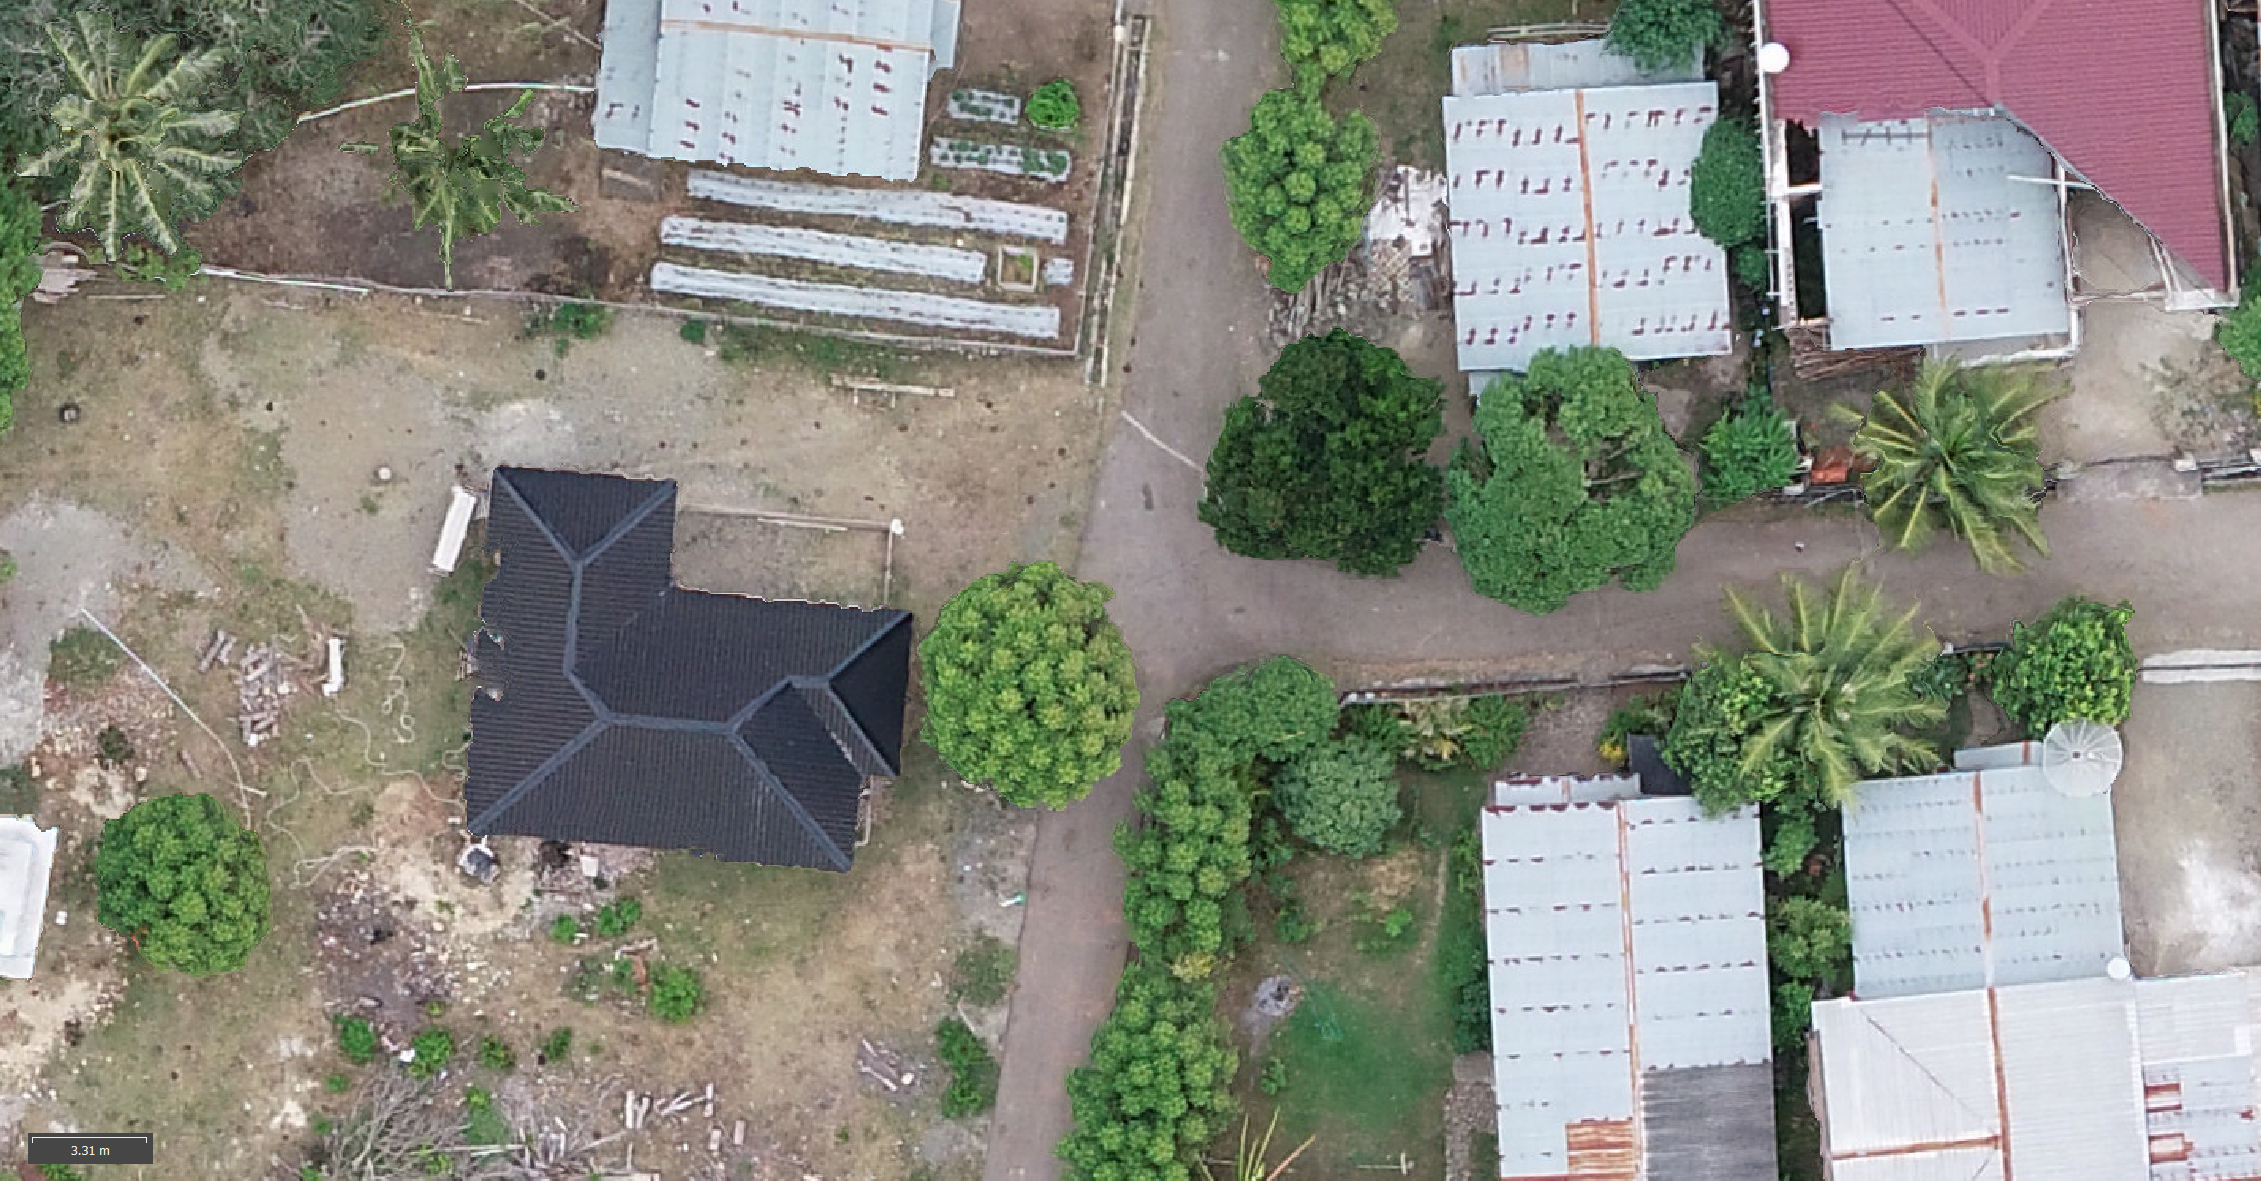
\includegraphics [width=1\linewidth]{image/agisoft perumahan.png}
    \caption{Hasil mosaik Agisoft Metashape di area perumahan}
    \label{visual perumahan 1}
\end{figure}

\begin{figure} [H]
    \centering
    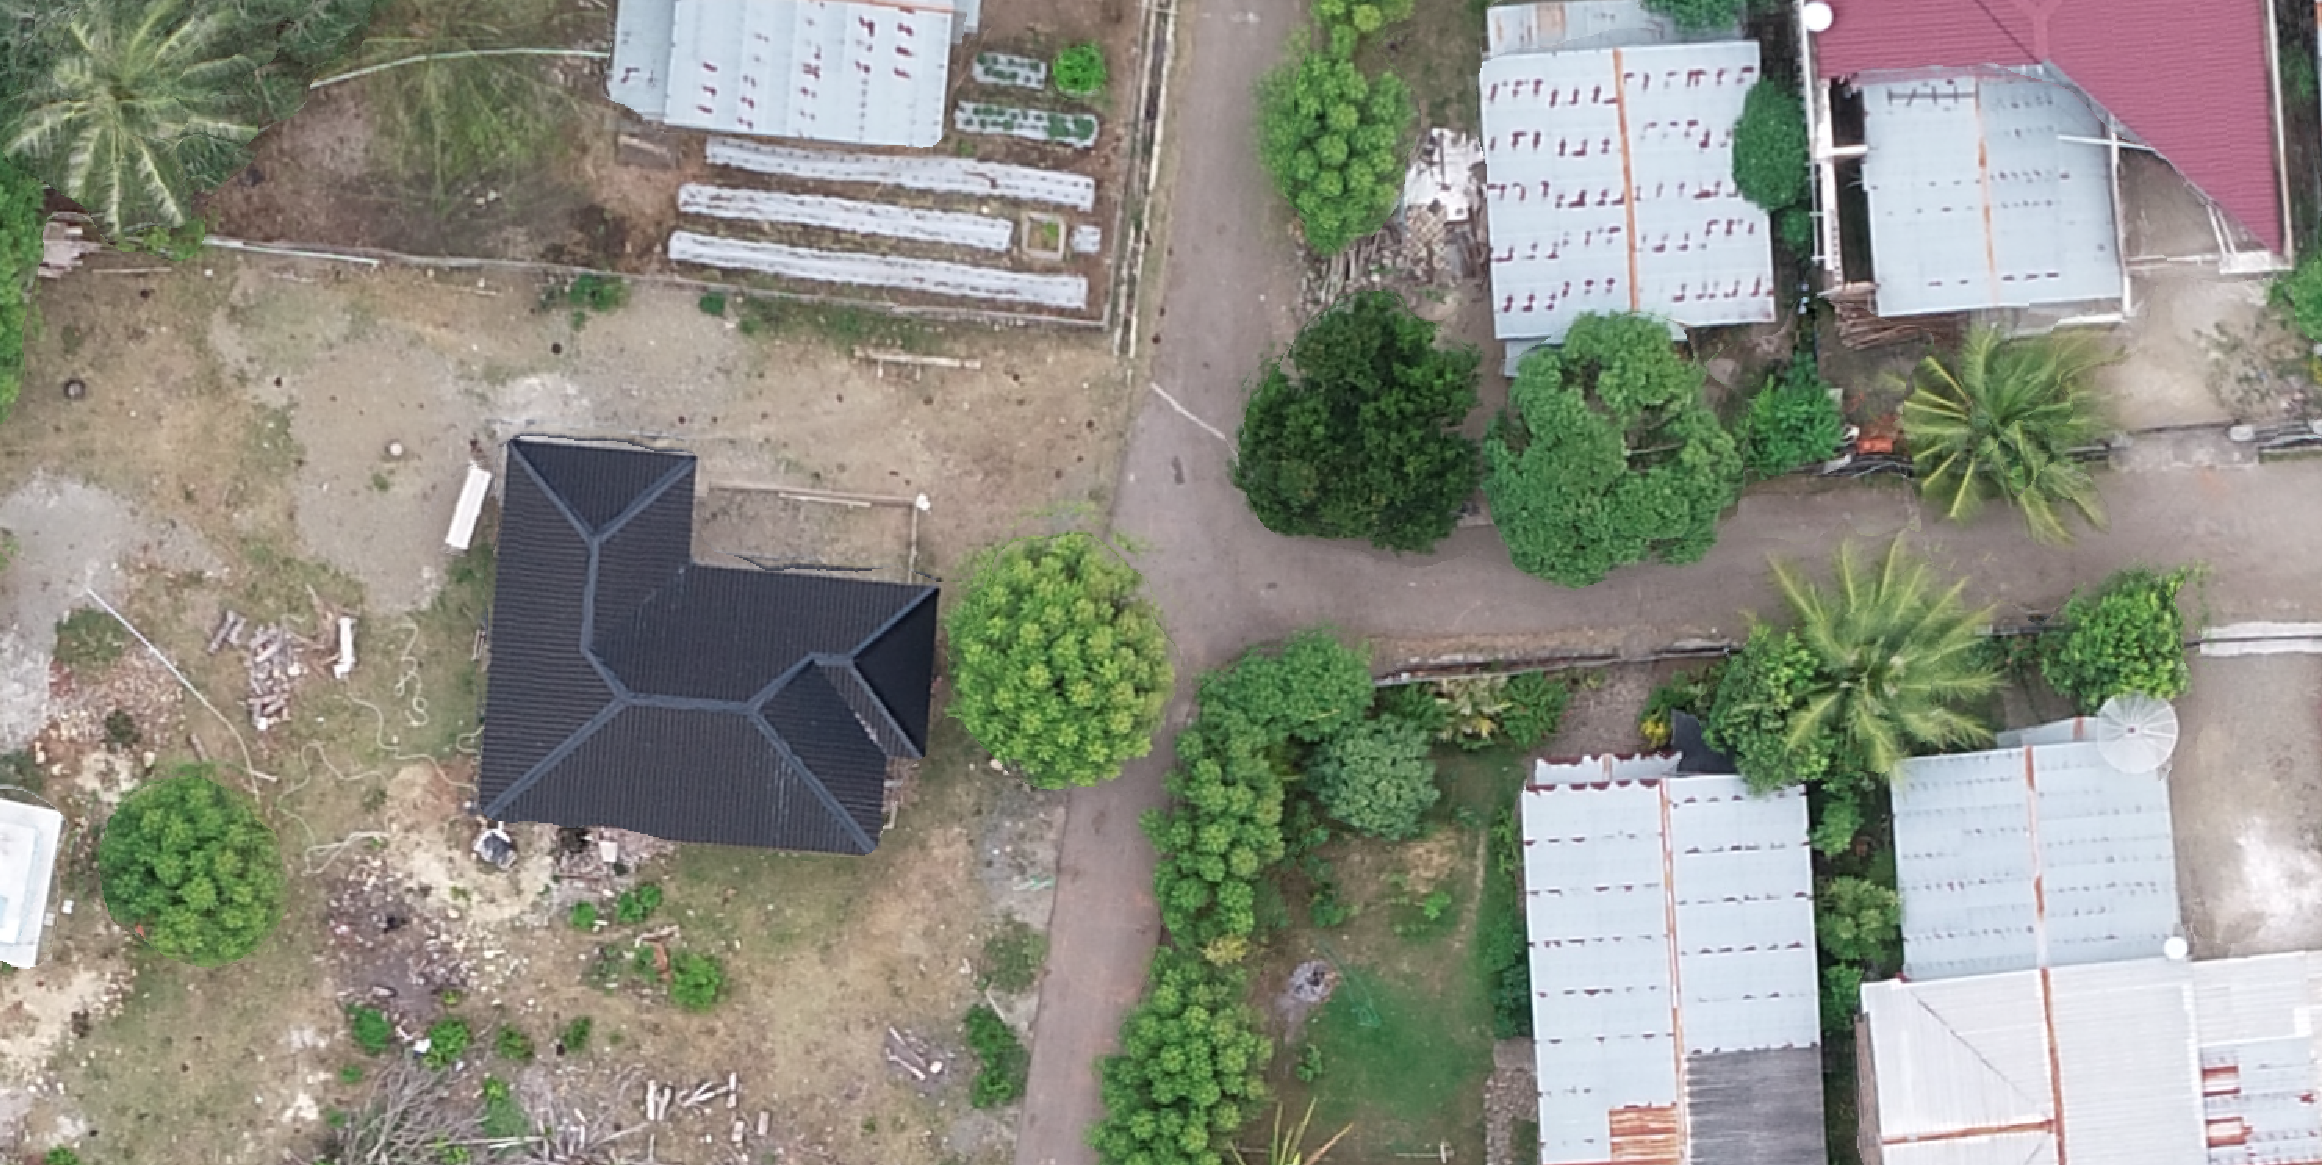
\includegraphics [width=1\linewidth]{image/pix perumahan.png}
    \caption{Hasil mosaik PIX4Dmapper di area perumahan}
    \label{visual perumahan 2}
\end{figure}

Dalam perbandingan hasil pengolahan citra mosaik di kawasan perumahan seperti pada Gambar \ref{visual perumahan 1} dan \ref{visual perumahan 2}, PIX4D Mapper menunjukkan keunggulan dibandingkan dengan Agisoft Metashape. Hasil dari Agisoft Metashape memperlihatkan beberapa kekurangan, terutama pada bagian ujung dan tepian atap rumah yang tampak bergerigi. Sebaliknya, PIX4D Mapper mampu menghasilkan rekonstruksi tepian atap dengan presisi tinggi dan detail yang sangat baik. Perlu dicatat bahwa perbedaan kualitas ini hanya terlihat pada beberapa area rumah tertentu, bukan pada keseluruhan citra.


\begin{figure} [H]
    \centering
    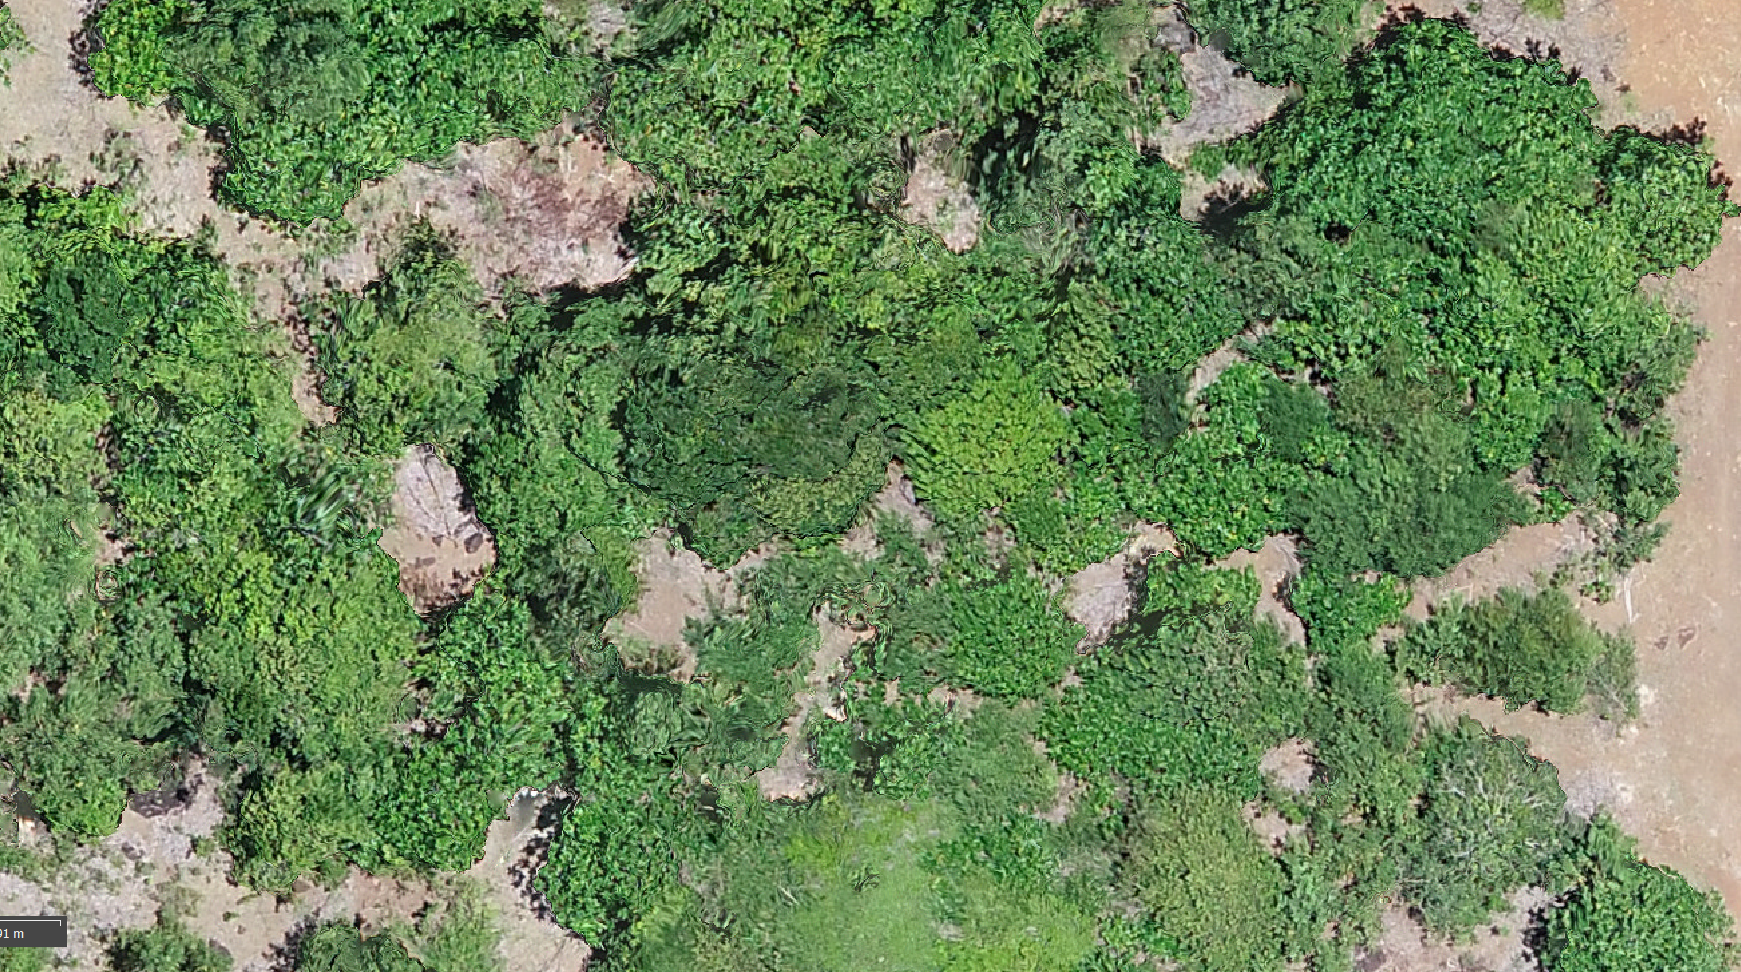
\includegraphics [width=1\linewidth]{image/agisoft vegetasi.png}
    \caption{Hasil mosaik Agisoft Metashape di area vegetasi}
    \label{visual vegetasi 1}
\end{figure}

\begin{figure} [H]
    \centering
    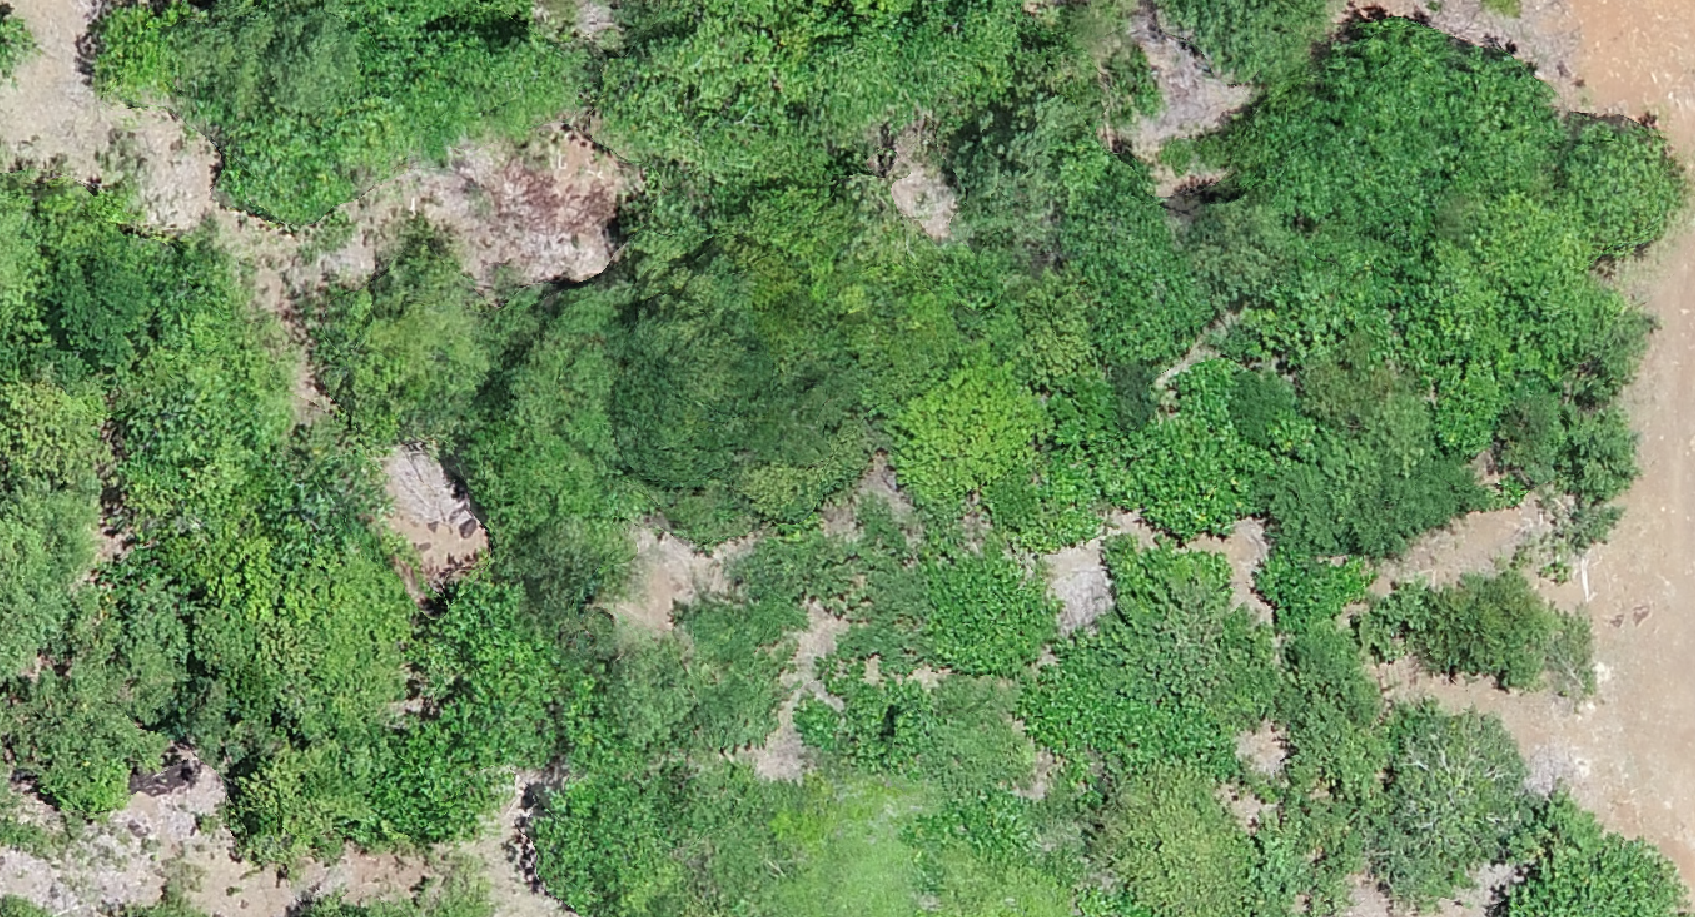
\includegraphics [width=1\linewidth]{image/pix vegetasi.png}
    \caption{Hasil mosaik PIX4Dmapper di area vegetasi}
    \label{visual vegetasi 2}
\end{figure}

Dalam perbandingan area vegetasi, Agisoft Metashape menghasilkan gambar yang lebih tajam, sementara PIX4D Mapper menghasilkan citra yang lebih halus. Meski demikian, hasil Agisoft Metashape menunjukkan beberapa kelemahan, seperti pohon yang tampak kabur dan daun yang menyatu. Pada hasil PIX4D Mapper, walaupun kurang tajam dalam detail namun berhasil memproses vegetasi secara lebih konsisten. Kedua perangkat lunak ini memiliki kelebihan dan kekurangan masing-masing dalam memvisualisasikan area bervegetasi.

\begin{figure} [H]
    \centering
    \includegraphics [width=1\linewidth]{image/lereng perbukitan agisoft.png}
    \caption{Hasil mosaik Agisoft Metashape di area lereng bukit}
    \label{visual lereng 1}
\end{figure}

\begin{figure} [H]
    \centering
    \includegraphics [width=1\linewidth]{image/lereng perbukitan pix.png}
    \caption{Hasil mosaik PIX4Dmapper di area lereng bukit}
    \label{visual lereng 2}
\end{figure}

Pada hasil mosaik di area lereng perbukitan, seperti yang ditunjukkan pada gambar \ref{visual lereng 1} dan \ref{visual lereng 2}, terlihat bahwa hasil dari Agisoft Metashape mengalami perubahan warna dan cahaya mendadak sehingga gambar tampak tidak menyatu. Sebaliknya, hasil dari PIX4D menunjukkan pengolahan gambar yang sangat baik tanpa ada masalah, menghasilkan mosaik yang lebih bagus dan konsisten.

\begin{figure} [H]
    \centering
    \includegraphics [width=1\linewidth]{image/jalan agisoft.png}
    \caption{Hasil mosaik Agisoft Metashape di area perkebunan}
    \label{visual jalan 1}
\end{figure}

\begin{figure} [H]
    \centering
    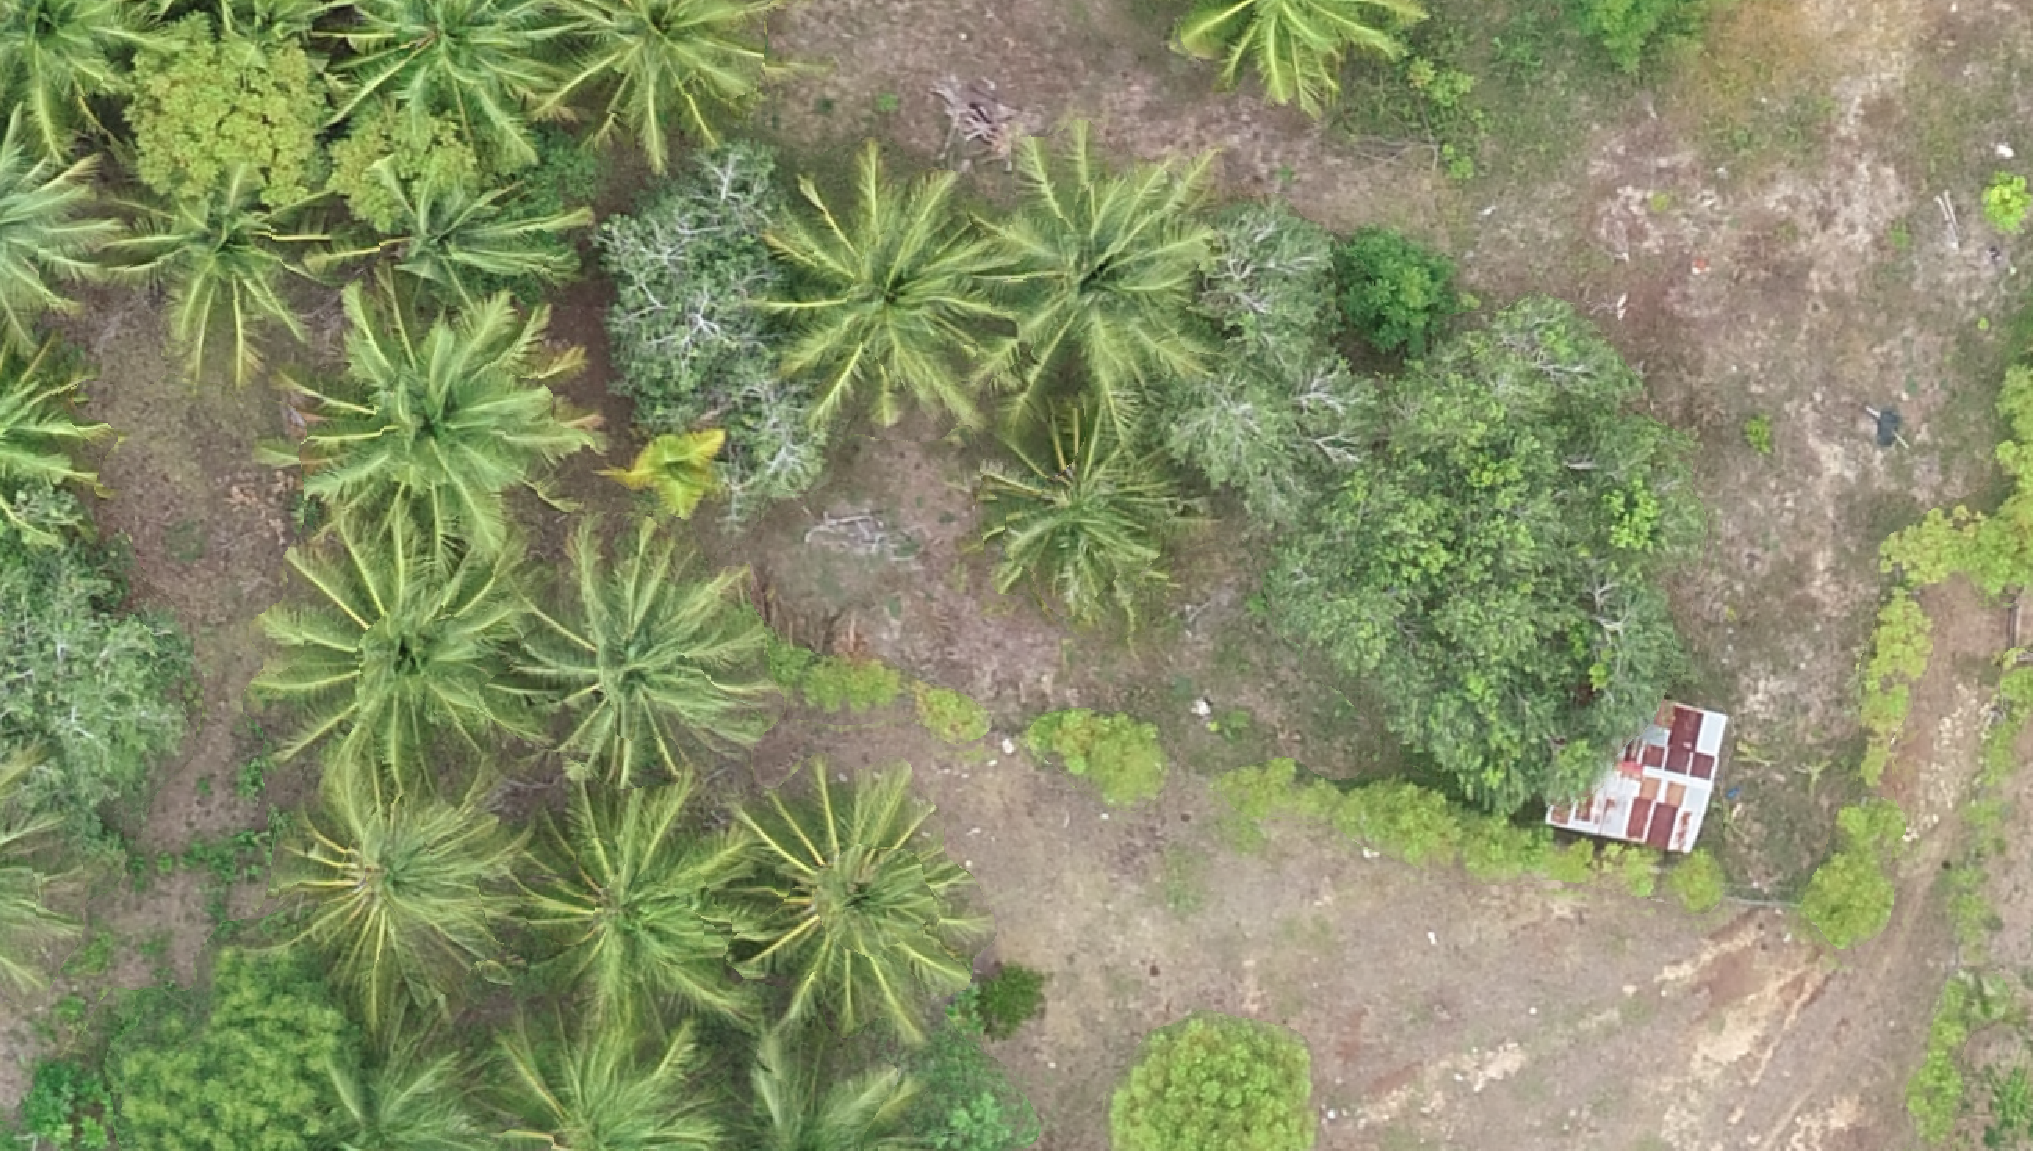
\includegraphics [width=1\linewidth]{image/jalan pix.png}
    \caption{Hasil mosaik PIX4Dmapper di area perkebunan}
    \label{visual jalan 2}
\end{figure}

Hasil mosaik pada area perkebunan, seperti yang terlihat pada Gambar \ref{visual jalan 1} dan \ref{visual jalan 2}, menunjukkan bahwa kedua perangkat lunak, Agisoft Metashape dan PIX4D Mapper, mampu menghasilkan gambar permukaan tanah dengan baik. Namun, keduanya menghadapi kesulitan dalam memproses bagian pohon kelapa, sehingga masih terdapat beberapa kekurangan pada hasil akhir.

\begin{figure} [H]
    \centering
    \includegraphics [width=1\linewidth]{image/bolong agisoft.png}
    \caption{Hasil mosaik Agisoft Metashape berlubang di area data yang rusak}
    \label{visual bolong 1}
\end{figure}

\begin{figure} [H]
    \centering
    \includegraphics [width=1\linewidth]{image/bolong pix.png}
    \caption{Hasil mosaik PIX4Dmapper berlubang di area data yang rusak}
    \label{visual bolong 2}
\end{figure}

Selain perbandingan visual, seperti yang terlihat pada Gambar \ref{visual bolong 1} dan \ref{visual bolong 2} terdapat data foto udara yang diduga rusak dan tidak dapat dikalibrasi selama proses pengaturan foto di kedua perangkat lunak. Kerusakan ini menyebabkan hilangnya foto udara di area tertentu, mengakibatkan adanya lubang pada hasil mosaik. Satu-satunya cara untuk memperbaiki data yang rusak ini adalah dengan mengambil ulang foto udara menggunakan drone di area yang sama
% Baris ini digunakan untuk membantu dalam melakukan sitasi
% Karena diapit dengan comment, maka baris ini akan diabaikan
% oleh compiler LaTeX.
\begin{comment}
\bibliography{daftar-pustaka}
\end{comment}

\fancyhf{} 
\fancyfoot[R]{\thepage}

%-------------------------------------------------------------------------------
%                            BAB V
%               		KESIMPULAN DAN SARAN
%-------------------------------------------------------------------------------
% \fancyhf{} 
% \fancyfoot[R]{\thepage}
\chapter{KESIMPULAN DAN SARAN}
%\thispagestyle{plain} % Halaman pertama bab menggunakan gaya plain

\section{Kesimpulan}

\section{Saran}


%-----------------------------------------------------------------------------%

% Baris ini digunakan untuk membantu dalam melakukan sitasi
% Karena diapit dengan comment, maka baris ini akan diabaikan
% oleh compiler LaTeX.
\begin{comment}
\bibliography{daftar-pustaka}
\end{comment}

\fancyhf{} 
\fancyfoot[C]{\thepage}



\fancypagestyle{daftarpustaka}{
    \fancyhf{} % Hapus semua header dan footer yang sudah ada
    \fancyfoot[C]{\thepage} % Letakkan nomor halaman di tengah kepala (center)
    \renewcommand{\headrulewidth}{0pt} % Hapus garis pemisah kepala dengan konten
    \renewcommand{\footrulewidth}{0pt} % Hapus garis pemisah footer dengan konten
}


% Halaman Daftar Pustaka dengan penomoran halaman berada di tengah dan nomor halaman selanjutnya di kanan
\addcontentsline{toc}{chapter}{DAFTAR PUSTAKA}
\begin{onehalfspace}
\begin{spacing}{1}
\pagestyle{daftarpustaka}
\bibliography{daftar-pustaka}
\end{spacing}
%-----------------------------------------------------------------
% Disini akhir masukan Daftar Pustaka
%-----------------------------------------------------------------

%%
% @author Kurnia Saputra
% @version 1.0
% 
% Hanya sebuah pembatas bertuliskan LAMPIRAN ditengah halaman. 
% 

\begin{titlepage}
	\centering 
	\vspace*{6cm}
	\noindent \Huge{LAMPIRAN}
	%\addChapter{LAMPIRAN}
	\addcontentsline{toc}{chapter}{LAMPIRAN}
\end{titlepage}
\addcontentsline{toc}{chapter}{LAMPIRAN}
\chapter*{LAMPIRAN}

\addcontentsline{toc}{chapter}{LAMPIRAN} %daftar lampiran

\end{onehalfspace}

\end{document}